%%%%%%%%%%%%%%%%%%%%%%%%%%%%%%%%%%%%%%%%%%%%%%%%%%%%%%%%%%%%%%%%%%%%%%%%%%%%%%%%%%%%%%%%%
% Khóa luận tốt nghiệp/Tiểu luận 
% LaTeX Template
% Phiên bản 1.0 (tạo ra ngày 05/10/2022)
%
% Template này có thể được download tại:
% https://github.com/cpc1996/HUS-Dissertation-Template
%%%%%%%%%%%%%%%%%%%%%%%%%%%%%%%%%%%%%%%%%%%%%%%%%%%%%%%%%%%%%%%%%%%%%%%%%%%%%%%%%%%%%%%%%


%----------------------------------------------------------------------------------------
%	(KHÔNG CHỈNH SỬA PHẦN NÀY)
%
%	PHẦN 1: CÁC PACKAGE CƠ BẢN VÀ CÁC TÙY CHỈNH VĂN BẢN
%----------------------------------------------------------------------------------------

\documentclass[
12pt,
oneside,
english,
doublespacing,
nolistspacing,
liststotoc,
parskip,
headsepline,
chapterinoneline,
]{HUSdissertation}

% \usepackage[utf8]{inputenc} 
\usepackage[utf8]{vietnam} 
%\usepackage[T1]{fontenc}

\usepackage{mathptmx}
\usepackage{amsmath}
\usepackage{graphicx} 
\usepackage{array}
\allowdisplaybreaks

%https://www.overleaf.com/learn/latex/Biblatex_citation_styles
%\usepackage[backend=bibtex,style=authoryear,natbib=true]{biblatex}
\usepackage[backend=bibtex,style=numeric,citestyle=ieee,natbib=true]{biblatex}

\addbibresource{main.bib}

\usepackage[autostyle=true]{csquotes}


%----------------------------------------------------------------------------------------
%	PHẦN 2: CÁC PACKAGE BỔ TRỢ THÊM VÀO TRONG QUÁ TRÌNH BIÊN SOẠN
%----------------------------------------------------------------------------------------

\RequirePackage{setlst}		% Liệt kê/trích dẫn code

\usepackage{multirow}
\usepackage{subfigure}
\usepackage[fontsize=13pt]{scrextend}

%https://www.sascha-frank.com/latex-font-size.html
%https://tex.stackexchange.com/questions/103286/how-to-change-section-subsection-font-size
\usepackage{titlesec}

\titleformat{\section}
{\normalfont\fontsize{13}{13}\bfseries}{\thesection}{1em}{}

\titleformat{\subsection}
{\normalfont\fontsize{13}{13}\bfseries\itshape}{\thesubsection}{1em}{}

%https://tex.stackexchange.com/questions/351961/how-to-indent-code-in-beginverbatim
\usepackage{fancyvrb} 		% Fancy Verbatim
\fvset{tabsize=4,vspace=0pt,fontsize=\footnotesize}

\usepackage{longtable} 		% Bảng dài - Long table

\usepackage[figuresright]{rotating} % Bảng ngang - Sideways table
\usepackage{tabularx}

\usepackage{fontawesome5} 	% Các biểu tượng, ký hiệu đặc biệt

\usepackage{tikz} 			% Vẽ hình
\usetikzlibrary{calc}

\usepackage{indentfirst}	% Lùi đầu dòng ở đầu đoạn văn
\setlength{\parindent}{0.5cm}

%----------------------------------------------------------------------------------------
%	PHẦN 3: THÔNG TIN VỀ Khóa luận tốt nghiệp/Tiểu luận (THESIS INFORMATION)
%----------------------------------------------------------------------------------------

\author{Nhóm 6} 			
\thesistitle{Human Activity Recognition} 

\supervisor {TS. Phạm Tiến Lâm} 
\supervisorr{Thầy Đặng Văn Báu} 

\field{Ngành Kỹ thuật Điện tử và Tin học} 				
\program{Chương trình đạo tạo chuẩn} 			
\doctype{Học phần Thị Giác Máy Tính} 

\university{\href{http://hus.vnu.edu.vn}{Trường Đại học Khoa học Tự nhiên}}
\department{\href{http://hus.vnu.edu.vn/gioi-thieu/co-cau-to-chuc/khoa-truc-thuoc/khoa-vat-ly.html}{Khoa Vật lý}}

\AtBeginDocument{
	\hypersetup{pdftitle=\ttitle}
	\hypersetup{pdfauthor=\authorname}
}


\begin{document}

\lstset{style=codeC}	% Thiết lập ngôn ngữ C/C++ là ngôn ngữ mặc định cho phần liệt kê souce code của cả bài

\frontmatter 			% Sử dụng hệ thống đánh số La Mã (i, ii, iii, iv...) cho những trang trước phần mục lục

\pagestyle{plain} 


%----------------------------------------------------------------------------------------
%	(KHÔNG CHỈNH SỬA PHẦN NÀY)
%
%	PHẦN 4: TRANG TIÊU ĐỀ/TRANG BÌA (TITLE PAGE)
%----------------------------------------------------------------------------------------

% TRANG BÌA CHÍNH:
%----------------------------------------------------------------------------------------
%	(KHÔNG CHỈNH SỬA PHẦN NÀY)
%
%	Phần 6: TRANG TIÊU ĐỀ/TRANG BÌA (TITLE PAGE)
%----------------------------------------------------------------------------------------

% TRANG BÌA CHÍNH:
\begin{titlepage}
	\begin{tikzpicture}[overlay,remember picture]
		\draw [line width=3pt]
		($ (current page.north west) + (2.0cm,-2.0cm) $)
		rectangle
		($ (current page.south east) + (-1.5cm,1.8cm) $);
		\draw [line width=1pt]
		($ (current page.north west) + (2.15cm,-2.15cm) $)
		rectangle
		($ (current page.south east) + (-1.65cm,1.95cm) $); 
	\end{tikzpicture}
	\begin{center}
		
		\vspace{-.04\textheight}
		\noindent%\scshape
		\large \, \href{https://www.vnu.edu.vn/home/}{ĐẠI HỌC QUỐC GIA HÀ NỘI}\\
		\vspace{-0.25cm}{\large \MakeUppercase \univname}\\
		\vspace{-0.25cm}{\large \bfseries \MakeUppercase \deptname}\\[0.5cm]
		
\includegraphics{Logo/Logo_HUS_notext_nocolor}
		
		\vspace{1.0cm}
		
		{\large \MakeUppercase \authorname}
		
		\vspace{2.5cm}
		
		{\Large \bfseries \MakeUppercase\ttitle\par}
		
		\vspace{2.5cm}
		
		{\normalsize \docname\\ \fieldname\\ (\progname)\\}
		
		\vfill
		
		\textbf{Hà Nội - \the\year{}}
	\end{center}
\end{titlepage}



% TRANG BÌA PHỤ:
%----------------------------------------------------------------------------------------
%	(KHÔNG CHỈNH SỬA PHẦN NÀY)
%
%	Phần 6: TRANG TIÊU ĐỀ/TRANG BÌA (TITLE PAGE)
%----------------------------------------------------------------------------------------

% TRANG BÌA PHỤ:
\begin{titlepage}
	\begin{tikzpicture}[overlay,remember picture]
		\draw [line width=3pt]
		($ (current page.north west) + (2.0cm,-2.0cm) $)
		rectangle
		($ (current page.south east) + (-1.5cm,1.8cm) $);
		\draw [line width=1pt]
		($ (current page.north west) + (2.15cm,-2.15cm) $)
		rectangle
		($ (current page.south east) + (-1.65cm,1.95cm) $); 
	\end{tikzpicture}
	\begin{center}
		
		\vspace{-.04\textheight}
		\noindent%\scshape
		\large \, \href{https://www.vnu.edu.vn/home/}{ĐẠI HỌC QUỐC GIA HÀ NỘI}\\
		\vspace{-0.25cm}{\large \MakeUppercase \univname}\\
		\vspace{-0.25cm}{\large \bfseries \MakeUppercase \deptname}\\[0.5cm]
		
\includegraphics{Logo/Logo_HUS_notext}
		
		\vspace{1.0cm}
		
		{\large \MakeUppercase \authorname}
		
		\vspace{2.5cm}
		
		{\Large \bfseries \MakeUppercase\ttitle\par}
		
		\vspace{2.5cm}
		
		{\normalsize \docname\\ \fieldname\\ (\progname)\\}
		
		\vspace{2.5cm}
		
		\begin{minipage}[t]{0.49\textwidth}
			\begin{flushright} \large \bfseries
				Giảng viên hướng dẫn:\;
			\end{flushright}
		\end{minipage}
		\begin{minipage}[t]{0.5\textwidth}
			\begin{flushleft} \large \bfseries
				\supname\\
				\supnamee
			\end{flushleft}
		\end{minipage}
		
		\vfill
		
		\textbf{Hà Nội - \the\year{}}
	\end{center}
\end{titlepage}



%----------------------------------------------------------------------------------------
%	PHẦN 6: LỜI CẢM ƠN (ACKNOWLEDGEMENTS)
%----------------------------------------------------------------------------------------

\begin{acknowledgements}
	\addchaptertocentry{\acknowledgementname}
	\thispagestyle{empty}
	
	Trên thực tế không có sự thành công nào mà không gắn liền với những sự giúp đỡ dù ít hay nhiều, dù trực tiếp hay gián tiếp từ những người xung quanh. Trong suốt quá trình học tập và làm việc tại giảng đường tới nay, nhóm 6 đã nhận được nhiều sự quan tâm, giúp đỡ từ các thầy cô, gia đình và bạn bè. Nhóm 6 xin gửi lời cảm ơn chân thành nhất đến \textbf{TS. Phạm Tiến Lâm} và \textbf{Thầy Đặng Văn Báu} đã tận tâm hướng dẫn nhóm qua những buổi thảo luận, thực hành về môn học. Thầy đã giúp nhóm tích lũy thêm nhiều kiến thức, kĩ năng để có cái nhìn toàn diện ,sâu sắc và tính thiết thực mà môn học mang đến.
	
	Kiến thức là vô hạn mà sự tiếp thu tri thức của mỗi người là khác nhau và còn tồn tại những hạn chế nhất định. Do đó, trong quá trình hoàn thành bài báo cáo này, chắc chắn không tránh khỏi những thiếu sót. Nhóm 6 rất mong nhận được những ý kiến đóng góp quý báu từ thầy để bài báo cáo của nhóm được hoàn thiện hơn.
      Thời gian trôi qua thật nhanh, mới ngày nào chúng em còn bỡ ngỡ bước vào môn học , được thầy dìu dắt, dạy bảo. Dưới sự giảng dạy tận tình, tâm huyết của thầy, chúng em đã được tiếp thu những kiến thức bổ ích, quý giá, giúp chúng em mở mang tầm hiểu biết, hoàn thiện bản thân và chuẩn bị hành trang vững vàng cho tương lai.Chúng em xin hứa sẽ tiếp tục học tập, rèn luyện, phấn đấu để xứng đáng với sự kỳ vọng của thầy.
	Nhóm 6 xin kính chúc thầy sức khỏe và thành công trên sự nghiệp giảng dạy.
	
	\textbf{Nhóm 6 xin chân thành cảm ơn!}
	
	\begin{flushright}
		
		Nguyễn Đình Quang - 20002155\\
		Nguyễn Mạnh Trung - 20002171\\
		Đào Ánh Dương - 20002112\\
		
	\end{flushright}
\end{acknowledgements}


%----------------------------------------------------------------------------------------
%	(KHÔNG CHỈNH SỬA PHẦN NÀY)
%
%	PHẦN 7: MỤC LỤC (LIST OF CONTENTS/FIGURES/TABLES PAGES)
%----------------------------------------------------------------------------------------

\begin{spacing}{1.15}
	\tableofcontents 	% In ra mục lục chính
\end{spacing}

\begin{spacing}{1.15}
	\listoffigures 		% In ra danh sách hình vẽ
\end{spacing}

%\begin{spacing}{1.15}
	%\listoftables		% In ra danh sách bảng
%\end{spacing}


%----------------------------------------------------------------------------------------
%	PHẦN 8: DANH SÁCH TÊN VIẾT TẮT (ABBREVIATIONS)
%----------------------------------------------------------------------------------------

\begin{abbreviations}{ll} % Thêm danh sách tên viết tắt (dưới dạng một bảng có 2 cột)

\textbf{CNN} & \textbf{C}onvolutional \textbf{N}eural \textbf{N}etwork\\
\textbf{I/O} & \textbf{I}nput \textbf{O}utput \\
\textbf{ROM} & \textbf{R}ead \textbf{O}nly \textbf{M}emory\\
\textbf{RAM} & \textbf{R}andom \textbf{A}ccess \textbf{M}emory\\
\textbf{CPU} & \textbf{C}entral \textbf{P}rocessing \textbf{U}nit\\


\end{abbreviations}


%----------------------------------------------------------------------------------------
%	PHẦN 9: NỘI DUNG/CÁC CHƯƠNG Khóa luận tốt nghiệp/Tiểu luận (THESIS CONTENT - CHAPTERS)
%----------------------------------------------------------------------------------------

\mainmatter % Bắt đầu đánh số trang (1,2,3...)

\pagestyle{plain}

% Hãy thêm những chương (chapter) của khóa luận/tiểu luận vào thư mục Chapters
% Hãy bỏ chú thích những dòng nếu bạn đã bổ sung những chương vào

\chapter*{MỞ ĐẦU}
\addcontentsline{toc}{chapter}{MỞ ĐẦU}

\label{Chapter0} 

Computer vision đã và đang đóng góp một vai trò quan trọng trong tất cả các lĩnh vực trên toàn thế giới, mỗi năm có hàng ngàn báo cáo khoa học về đề tài này. Các công ty công nghệ hàng đầu như Google, Facebook, Amazon và Microsoft đang đầu tư mạnh mẽ vào học máy để phát triển các sản phẩm và dịch vụ mới. Ngoài ra, học máy cũng đang được sử dụng rộng rãi trong các lĩnh vực như y tế, tài chính, sản xuất và nhiều lĩnh vực khác để cải thiện hiệu suất và tối ưu hóa quy trình.

Những năm gần đây, khi mà khả năng tính toán của các máy tính được nâng lên một tầm cao mới và lượng dữ liệu khổng lồ được thu thập, Machine Learning đã tiến thêm một bước dài và Deep Learning ra đời. Deep Learning đã giúp máy tính thực thi những công việc phức tạp hơn như: phân loại cả ngàn vật thể trong các bức ảnh, tạo chú thích cho ảnh, bắt chước giọng nói và chữ viết của con người, giao tiếp với con người...

Nhận dạng hoạt động của con người (Human Activity Recognition – HAR) là một lĩnh vực nghiên cứu thú vị về thị giác máy tính và tương tác giữa người với máy.

HAR mang lại nhiều ứng dụng có ích cho cuộc sống con người. Theo dõi sức khỏe có thể được thực hiện thông qua các thiết bị đeo theo dõi hoạt động thể chất, nhịp tim và chất lượng giấc ngủ. Trong nhà thông minh, các giải pháp dựa trên HAR cho phép tiết kiệm năng lượng và tạo sự thoải mái cho cá nhân bằng cách phát hiện khi một người ra vào phòng và điều chỉnh ánh sáng hoặc nhiệt độ. Các thiết bị an toàn cá nhân có thể tự động cảnh báo các dịch vụ khẩn cấp hoặc một số liên lạc được chỉ định. Và đó chỉ là phần nổi của tảng băng chìm.

Với nhiều bộ dữ liệu có sẵn được chia sẻ công khai, việc tìm kiếm dữ liệu phục vụ mục đích nghiên cứu và phát triển HAR là rất đơn giản. Trong bài này này, Nhóm 6 sẽ cùng bạn tìm hiểu thêm về công nghệ tiên tiến nhất hiện nay của HAR, cùng với các phương pháp học sâu và bộ dữ liệu mở hỗ trợ tác vụ.


 

Nội dung chính của báo cáo có 5 chương:

Chương 1: Tổng quan về đề tài

Chương 2: Cơ sở lý thuyết dùng để giải quyết bài toán

Chương 3: Human Activity Recognition 

Chương 4: Demo sản phẩm và đánh giá các phương pháp

Chương 5: Kết luận  
 



% Chương 1

\chapter{TỔNG QUAN VỀ ĐỀ TÀI} 

\label{Chapter1} 

%----------------------------------------------------------------------------------------

% Định nghĩa một số lệnh cần thiết để điều chỉnh định dạng cho một số nội dung nhất định trong bài
\newcommand{\keyword}[1]{\textbf{#1}}
\newcommand{\tabhead}[1]{\textbf{#1}}
\newcommand{\code}[1]{\texttt{#1}}
\newcommand{\file}[1]{\texttt{\bfseries#1}}
\newcommand{\option}[1]{\texttt{\itshape#1}}

%----------------------------------------------------------------------------------------


\section{Khái niệm Thị giác máy tính (Computer Vision)}

hị giác máy tính là một công nghệ mà máy sử dụng để tự động nhận biết và mô tả hình ảnh một cách chính xác và hiệu quả. Ngày nay, các hệ thống máy tính có quyền truy cập vào khối lượng lớn hình ảnh và dữ liệu video bắt nguồn từ hoặc được tạo bằng điện thoại thông minh, camera giao thông, hệ thống bảo mật và các thiết bị khác. Ứng dụng thị giác máy tính sử dụng trí tuệ nhân tạo và máy học (AI/ML) để xử lý những dữ liệu này một cách chính xác nhằm xác định đối tượng và nhận diện khuôn mặt, cũng như phân loại, đề xuất, giám sát và phát hiện.

\begin{figure}[h!]
	\centering
	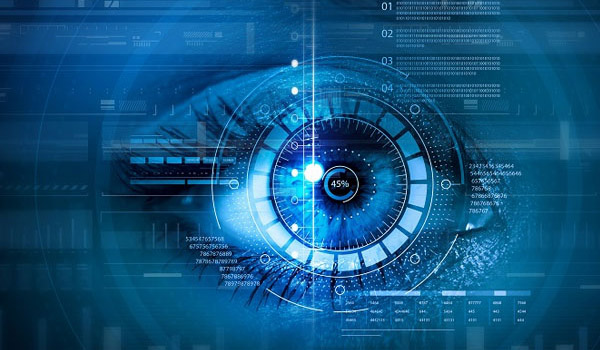
\includegraphics[width=0.65\textwidth]{computer-vision-la-gi.jpg}
	\caption[Computer Vision.]{Computer Vision.}
	\label{fig:ML}
\end{figure} 

Tuy rằng công nghệ xử lý thông tin hình ảnh đã xuất hiện từ lâu nhưng phần lớn quy trình vẫn đòi hỏi sự can thiệp của con người, tốn nhiều thời giờ và dễ bị lỗi. Ví dụ: việc triển khai hệ thống nhận diện khuôn mặt trước đây yêu cầu nhà phát triển phải gắn thẻ thủ công hàng ngàn hình ảnh bằng các điểm dữ liệu chính, chẳng hạn như chiều rộng sống mũi và khoảng cách giữa hai mắt. Tự động hóa các tác vụ này đòi hỏi sức mạnh điện toán rộng lớn vì dữ liệu hình ảnh không có cấu trúc và phức tạp để máy tính có thể sắp xếp. Do đó, ứng dụng thị giác tốn kém và hầu hết các tổ chức không thể tiếp cận.

Ngày nay, tiến bộ trong lĩnh vực này kết hợp với sự tăng cường đáng kể của sức mạnh điện toán đã cải thiện cả quy mô và độ chính xác của quy trình xử lý dữ liệu hình ảnh. Các hệ thống thị giác máy tính được hỗ trợ bởi tài nguyên điện toán đám mây hiện giờ trở nên dễ tiếp cận với tất cả mọi người. Bất kỳ tổ chức nào cũng có thể sử dụng công nghệ này để xác minh danh tính, kiểm duyệt nội dung, phân tích video phát trực tuyến, phát hiện lỗi và nhiều tính năng khác.

\section{Các trường hợp sử dụng của thị giác máy tính là gì?}
Nhiều ứng dụng thị giác máy tính được sử dụng trong lĩnh vực giải trí, kinh doanh, chăm sóc sức khỏe, giao thông vận tải và cuộc sống hàng ngày. Hãy cùng xem xét một số trường hợp sử dụng dưới đây:
\begin{itemize}
	\item Bảo mật và an toàn
	
	\item Hiệu quả hoạt động

	
	\item Chăm sóc sức khỏe
 
        \item Phương tiện tự hành
        

\end{itemize}

\section{Human Activity Recognition là gì? }

Human Activity Recognition (HAR) là một nhánh của ngành khoa học máy tính, với mục tiêu là tạo ra các hệ thống và kỹ thuật có khả năng tự động nhận dạng và phân loại các hành động của con người dựa trên dữ liệu cảm biến. HAR sử dụng các cảm biến để giải thích các cử chỉ hoặc chuyển động của cơ thể con người và xác định hoạt động hoặc chuyển động của con người.

Các hệ thống HAR thường được sử dụng trong nhiều ứng dụng khác nhau, bao gồm chăm sóc sức khỏe, vận động, an ninh, biểu diễn thể thao, v.v.

Trong khi xây dựng mô hình, mục tiêu của hệ thống HAR là dự báo nhãn hành động của một người trong hình ảnh hoặc video, thường được thực hiện thông qua nhận dạng hoạt động dựa trên video và nhận dạng hoạt động dựa trên hình ảnh.
\newpage

\section{HAR hoạt động như thế nào?} 

\begin{figure}[h!]
	\centering
	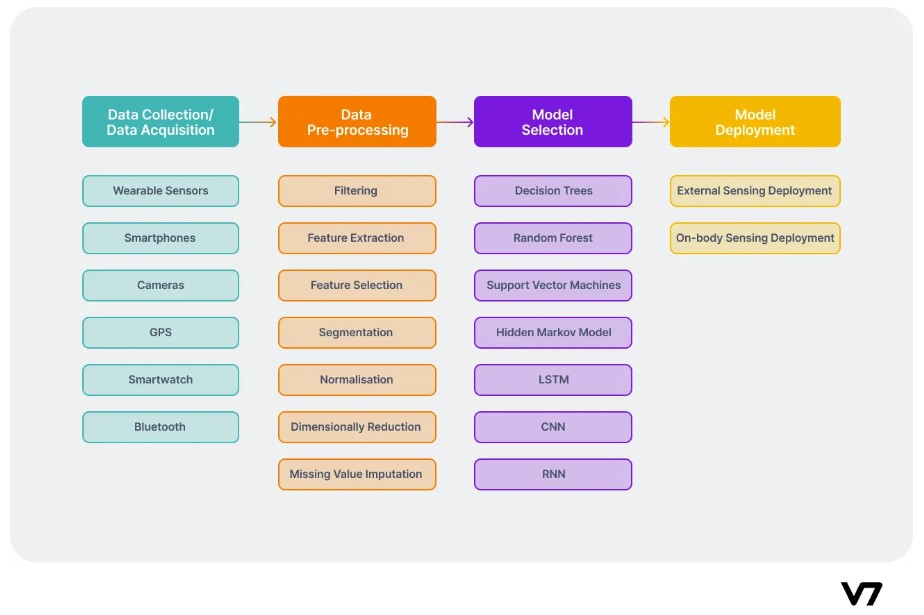
\includegraphics[width=0.65\textwidth]{Figures/flowchart.jpg}
	\caption[Flow Chart.]{Flow Chart.}
	\label{fig:ML}
\end{figure} 

\subsection{Mô tả bài toán thực tế} 

\begin{itemize}
	\item Sử dụng mạng CNN và LSTM để huấn luyện một mô hình có thể nhận biết hành động dựa vào webcam hoặc video  
	
	\item Đưa hành động vào webcam hoặc video chứa hành hành động vào model để dự đoán 

\end{itemize}

\subsection{Hướng tiếp cận bài toán }

\begin{itemize}
	\item Sử dụng thư viện MediaPipe và mạng LSTM với đầu vào là hành động trước webcam và đầu ra là phân loại hành động đó
	
	\item Sử dụng lớp layer ConvLSTM 
        \item Xây dựng mô hình LRCN
 

\end{itemize}


% Chương 2

\chapter{CƠ SỞ LÝ THUYẾT DÙNG ĐỂ GIẢI QUYẾT BÀI TOÁN} 

\label{Chapter2}

\section{Mạng neural tích chập (Convolutional Neural Network - CNN)}

\subsection{Khái niệm}

Mạng neural tích chập (Convolutional Neural Network - CNN) là một loại mạng neural sử dụng trong lĩnh vực xử lý ảnh và nhận dạng. Nó sử dụng các lớp tích chập để trích xuất đặc trưng từ ảnh đầu vào và áp dụng các lớp kết nối đầy đủ để phân loại ảnh. 

\begin{figure}[h!]
	\centering
	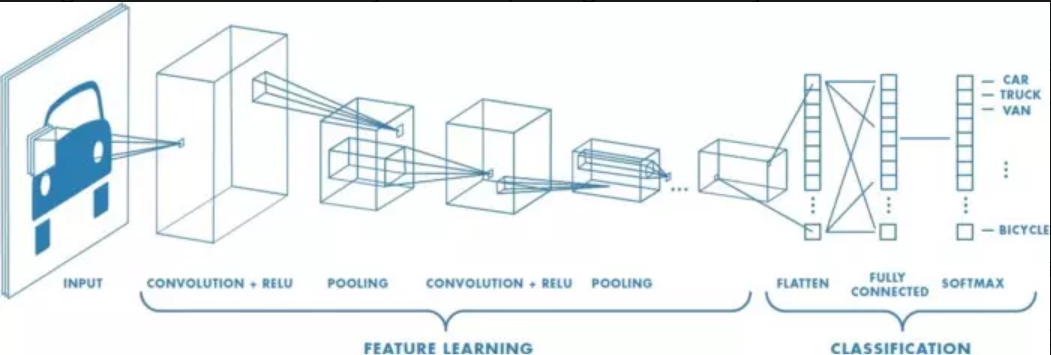
\includegraphics[width=0.8\textwidth]{CNN.png}
	\caption[Toàn bộ luồng CNN để xử lý hình ảnh đầu vào và phân loại các đối tượng dựa trên giá trị.]{Toàn bộ luồng CNN để xử lý hình ảnh đầu vào và phân loại các đối tượng dựa trên giá trị.}
	\label{fig:CNN} 
\end{figure}

Về kỹ thuật, mô hình CNN để training và kiểm tra, mỗi hình ảnh đầu vào sẽ chuyển nó qua 1 loạt các lớp tích chập với các bộ lọc (Kernel), tổng hợp lại các lớp được kết nối đầy đủ (Full Connected) và áp dụng hàm Softmax để phân loại đối tượng có giá trị xác suất giữa 0 và 1. Hình dưới đây là toàn bộ luồng CNN để xử lý hình ảnh đầu vào và phân loại các đối tượng dựa trên giá trị.

\begin{figure}[h!]
	\centering
	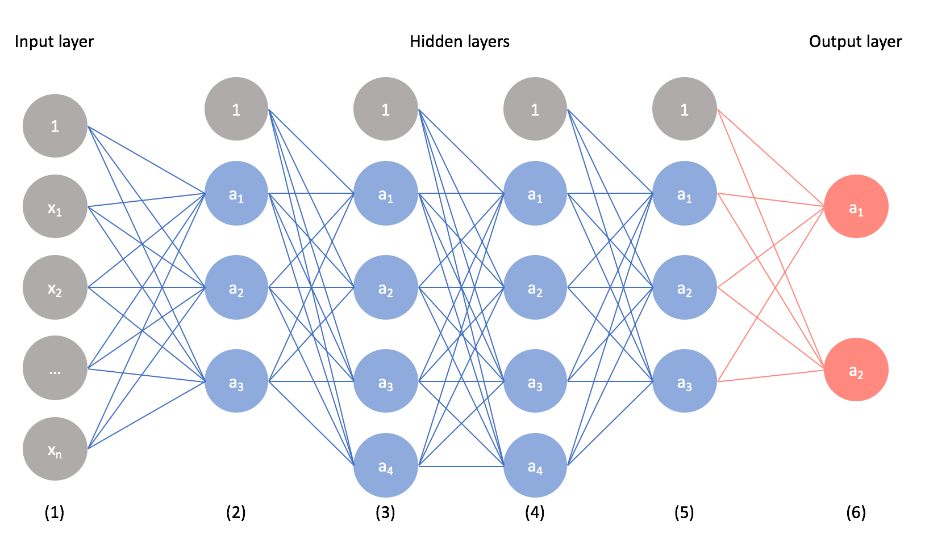
\includegraphics[width=0.7\textwidth]{anh2.png}
	\caption[Mô hình cấu trúc của mạng CNN.]{Mô hình cấu trúc của mạng CNN.}
	\label{fig:anh2} 
\end{figure}

\subsection{Feature trong CNN}

Các feature (đặc trưng) được sử dụng để trích xuất thông tin từ ảnh đầu vào. Các feature này được học tự động từ dữ liệu và được sử dụng để giảm thiểu số lượng thông tin cần xử lý trong quá trình huấn luyện mạng. 

Các feature này có thể là các đường cạnh, các vùng sáng tối, các đường cong và các đối tượng phức tạp hơn. 

Các feature này được trích xuất thông qua các bộ lọc tích chập và được kết hợp lại để tạo thành các feature maps, đóng vai trò quan trọng trong việc phân loại ảnh. Các feature maps này được đưa vào các lớp kết nối đầy đủ để phân loại ảnh đầu vào.

\subsection{Những lớp cơ bản của mạng CNN}

\subsubsection{Convolutional Layer}

Phần quan trọng nhất của toàn mạng CNN, các yếu tố quan trọng trong lớp Convolutional là: padding, stride, feature map và filter map.

\begin{itemize}
	\item Mạng CNN sử dụng filter để áp dụng vào các vùng của ma trận hình ảnh. Các filter map là các ma trận 3 chiều, bên trong đó là những tham số và chúng được gọi là parameters.
	
	\item Stride: dịch chuyển filter map theo từng pixel dựa vào các giá trị từ trái qua phải.
	
	\item Padding: Giá trị viền xung quanh của ma trận hình ảnh sẽ được gán các giá trị 0 để có thể tiến hành nhân tích chập ma trận mà không làm giảm kích thước ma trận ảnh ban đầu.
	
	\item Feature map: Biểu diễn kết quả sau mỗi lần feature map quét qua ma trận ảnh đầu vào. Sau mỗi lần quét thì lớp Convolutional sẽ tiến hành tính toán.
\end{itemize}

\begin{figure}[h!]
	\centering
	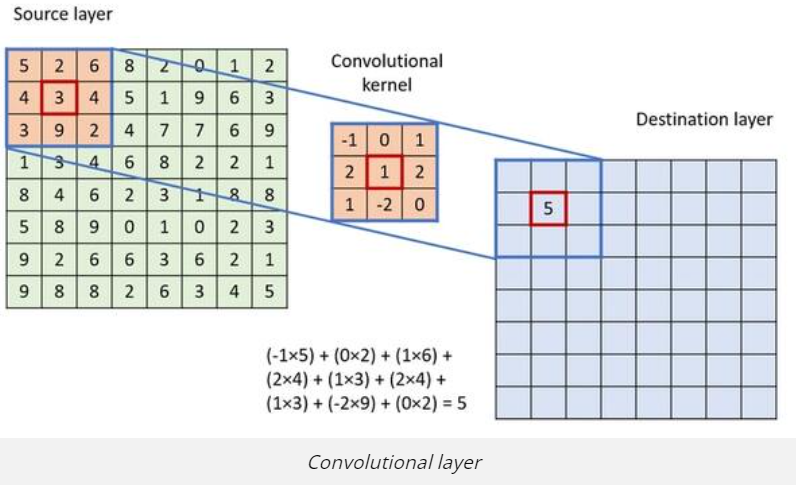
\includegraphics[width=0.7\textwidth]{convolution.png}
	\caption[Convolutional Layer.]{Convolutional Layer.}
	\label{fig:convolution} 
\end{figure}

\subsubsection{ReLU Layer}

Lớp ReLU là hàm kích hoạt trong mạng CNN, được coi là activation function. Nó có tác dụng mô phỏng những nơ ron có tỷ lệ truyền xung qua axon và hỗ trợ tính toán nhanh hơn.

Trong quá trình dùng hàm ReLU, chú ý đến việc tùy chỉnh learning rate và dead unit. Những lướp ReLU được dùng sau khi filter map được tính và áp dụng ReLU lên các giá trị của filter map.

\subsubsection{Pooling Layer}

Khi ma trận ảnh đầu vào có kích thước quá lớn, các lớp Pooling layer sẽ được đặt vào giữa những lớp Convolutional để làm giảm những parameters. Hai loại Pooling được sửu dụng phổ biến: Max pooling và Average.

\subsubsection{Fully Connected Layer}

Lớp có nhiệm vụ đưa ra kết quả sau khi 2 lớp Convolutional và Pooling đã nhận được ảnh truyền, khi này, ta sẽ thu được một model đọc được thông tin của ảnh.

\subsection{Kiến trúc của mạng CNN}

Mạng CNN là tập hợp những Convolutional layer xếp chồng lên nhau, đồng thời mạng sử dụng những hàm như ReLU và Tanh để kích hoạt các trọng số trong các node. Các lớp này sau khi qua các hàm activation sẽ có trọng số trong những node và có thể tạo ra những thông tin trừu tượng hơn đến với các lớp kế tiếp trong mạng.  

Cấu trúc cơ bản của một mô hình CNN:

\begin{itemize}
	\item Local receptive: Lớp này sử dụng để tách lọc dữ liệu, thông tin hình ảnh để từ đó có thể lựa chọn các vùng có giá trị sử dụng hiệu quả cao nhất.
	
	\item Shared weights field: Lớp này hỗ trợ làm giảm các tham số đến mức tối thiểu trong mạng CNN. Trong từng lớp convolution sẽ chứa các feature map riêng và từng feature thì sẽ có khả năng phát hiện một vài feature trong hình ảnh.
	
	\item Pooling layer: Lớp cuối cùng và sử dụng để làm đơn giản các thông tin output. Sau khi tính toán xong và quét qua các layer trong mạng thì pooling layer sẽ được dùng để lược bỏ các thông tin không hữu ích.
\end{itemize}
\section{Mạng hồi quy RNN}
Con người không bắt đầu suy nghĩ của họ từ đầu tại tất cả các thời điểm. Cũng như bạn đang đọc bài viết này, bạn hiểu mỗi chữ ở đây dựa vào từ bạn đã hiểu các chữ trước đó chứ không phải là đọc tới đâu ném hết đi tới đó, rồi lại bắt đầu suy nghĩ lại từ đầu tới chữ bạn đang đọc. Tức là tư duy đã có một bộ nhớ để lưu lại những gì diễn ra trước đó.

Tuy nhiên các mô hình mạng nơ-ron truyền thống thì không thể làm được việc đó, đó có thể coi là một khuyết điểm chính của mạng nơ-ron truyền thống. Ví dụ, bạn muốn phân loại các bối cảnh xảy ra ở tất cả các thời điểm trong một bộ phim, thì đúng là không rõ làm thế nào để có thể hiểu được một tình huống trong phim mà lại phụ thuộc vào các tình huống trước đó nếusử dụng các mạng nơ-ron truyền thống.

Mạng nơ-ron hồi quy (Recurrent Neural Network) sinh ra để giải quyết vấn đề đó. Mạng này chứa các vòng lặp bên trong cho phép thông tin có thể lưu lại được.
\begin{figure}[h!]
	\centering
	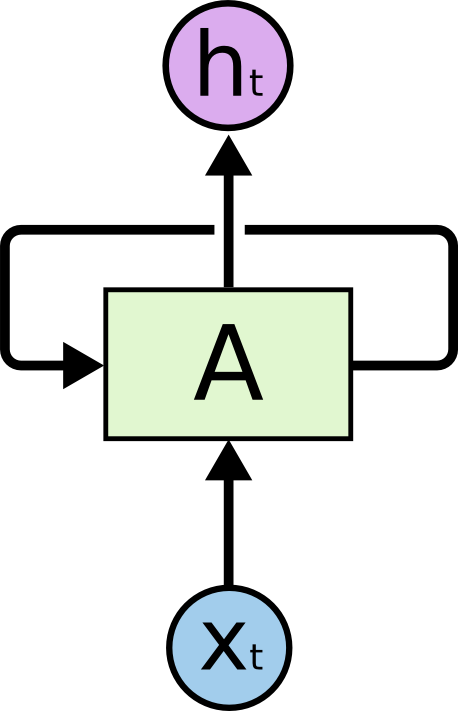
\includegraphics[width=0.7\textwidth]{Figures/RNN-rolled.png}
	\caption[Một đoạn RNN.]{Một đoạn RNN.}
	\label{fig:RNN-rolled.png} 
\end{figure}
Hình vẽ trên mô tả một đoạn của mạng nơ-ron hồi quy A với đầu vào là \( x_{t} \) và đầu ra là \( h_{t} \).Một vòng lặp cho phép thông tin có thể được truyền từ bước này qua bước này qua bước khác của mạng nơ-ron.

Các vòng lặp này khiến cho mạng nơ-ron hồi quy trông có vẻ khó hiểu. Tuy nhiên, nếu bạn để ý một chút thì nó không khác mấy so với các mạng nơ-ron thuần. Một mạng nơ-ron hồi quy có thể được coi là nhiều bản sao chép của cùng một mạng, trong đó mỗi đầu ra của mạng này là đầu vào của một mạng sao chép khác. Nói thì hơi khó hiểu, nhưng bạn hãy xem hình mô tả sau:
\begin{figure}[h!]
	\centering
	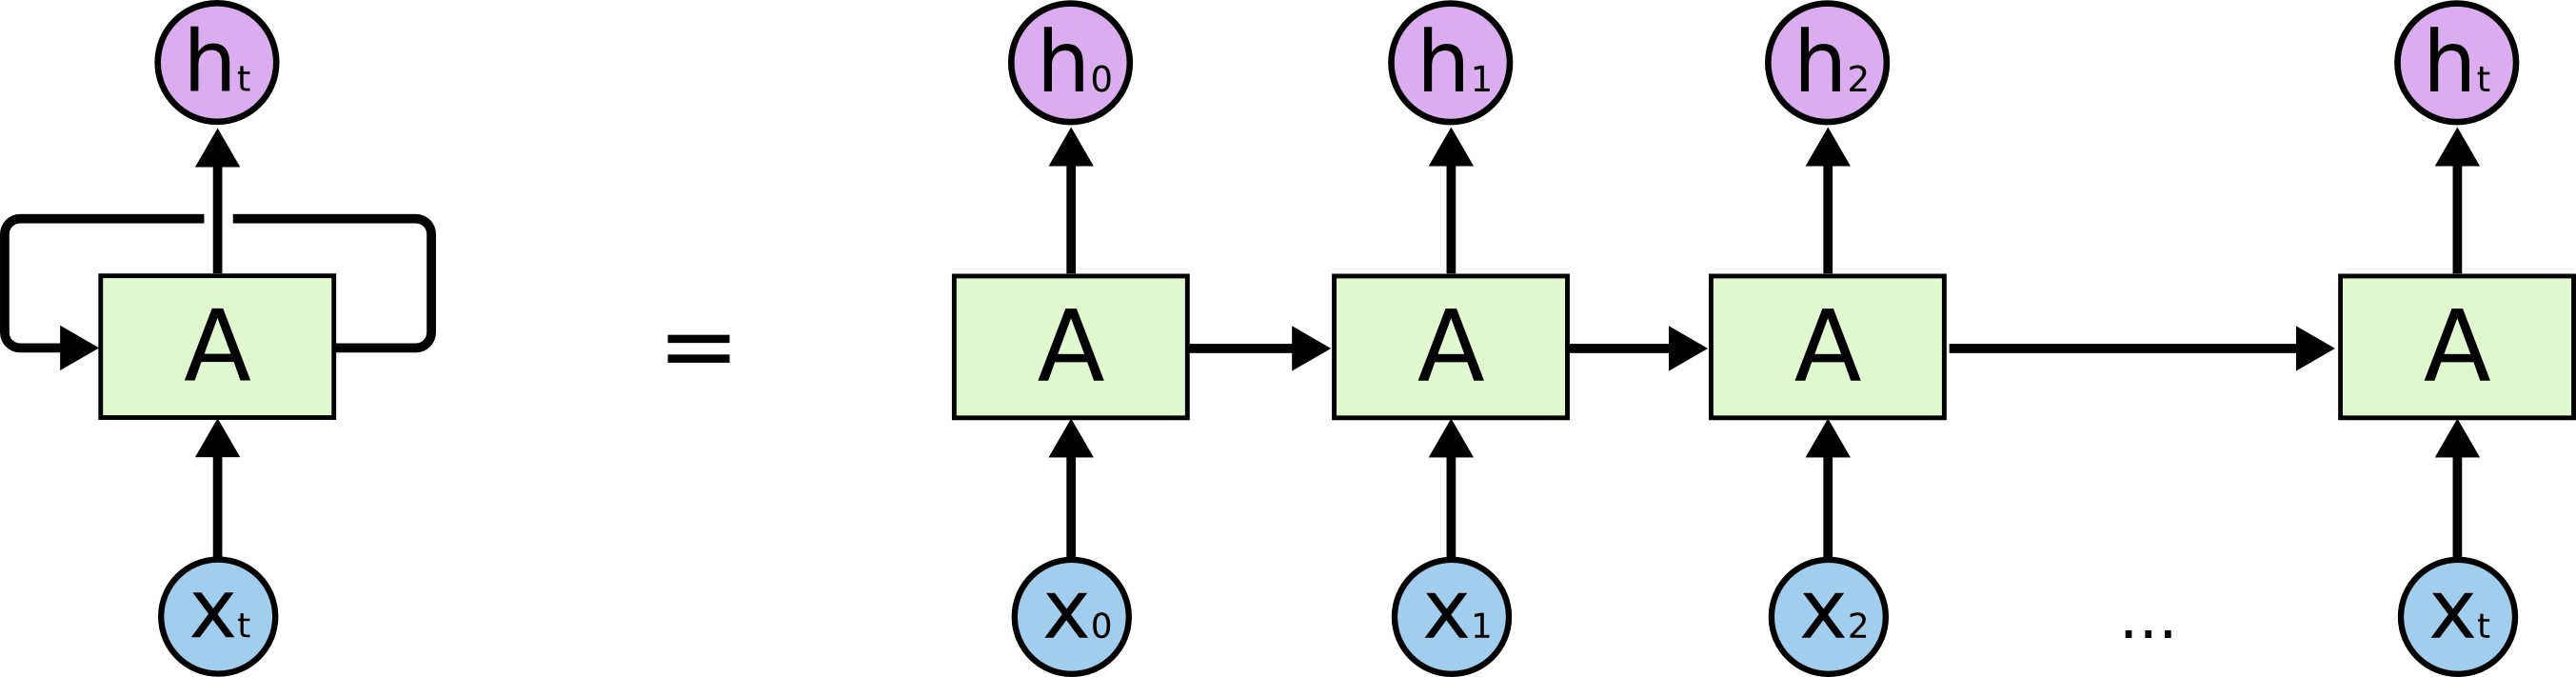
\includegraphics[width=0.7\textwidth]{Figures/RNN-unrolled.png}
	\caption[Mạng RNN.]{Mạng RNN.}
	\label{fig:RNN-unrolled.png} 
\end{figure}
Chuỗi lặp lại các mạng này chính là phân giải của mạng nơ-ron hồi quy, các vòng lặp khiến chúng tạo thành một chuỗi danh sách các mạng sao chép nhau. Bạn có thấy nó khác gì một mạng nơ-ron thuần không? Không khác gì phải không? Các nút của mạng vẫn nhận đầu vào và có đầu ra hệt như mạng nơ-ron thuần.

Trong vài năm gần đây, việc ứng dụng RNN đã đưa ra được nhiều kết quả không thể tin nổi trong nhiều lĩnh vực: nhận dạng giọng nói, mô hình hóa ngôn ngữ, dịch máy, mô tả ảnh,… Danh sách vẫn còn đang được mở rộng tiếp. Anh Andrej Karpathy đã đề cập tới một số kêt quả mà RNN mang lại tại bài viết này, nên tôi sẽ không bàn luận thêm nữa. Nhưng tôi vẫn muốn thốt lên rằng chúng thật là quá tuyệt vời.

Đằng sau sự thành công này chính là sự đóng góp của LSTM. LSTM là một dạng đặc biệt của mạng nơ-ron hồi quy, với nhiều bài toán thì nó tốt hơn mạng hồi quy thuần. Hầu hết các kết quả thú vị thu được từ mạng RNN là được sử dụng với LSTM. Trong bài viết này, ta sẽ cùng khám phá xem mạng LSTM là cái gì nhé.
\section{Mạng LSTM}
Mạng nơ-ron LSTM( Long Short-Term Memory là một loại mạng nơ ron hồi quy RNN được thiết kế đặc biệt để giải quyết vấn đề biến mất đường hồi quy (vanishing grandient) trong việc xử lý chuỗi liên tục . Biến mất đường hồi quy là hiện tượng khi gradient trong quá trình lan truyền ngược giảm đi rất nhanh , gây khó khăn trong việc  học các phụ thuộc xa trong dữ liệu chuỗi . LSTM đã được giới thiệu vào năm 1997 bởi Sep Hochreiter và Jurgen Schmidhuber và từ đó trở thành một trong những mô hình RNN phổ biến nhất và hiệu quả nhất . 

\subsubsection{Tổng quan về LSTM}

\begin{figure}[h!]
	\centering
	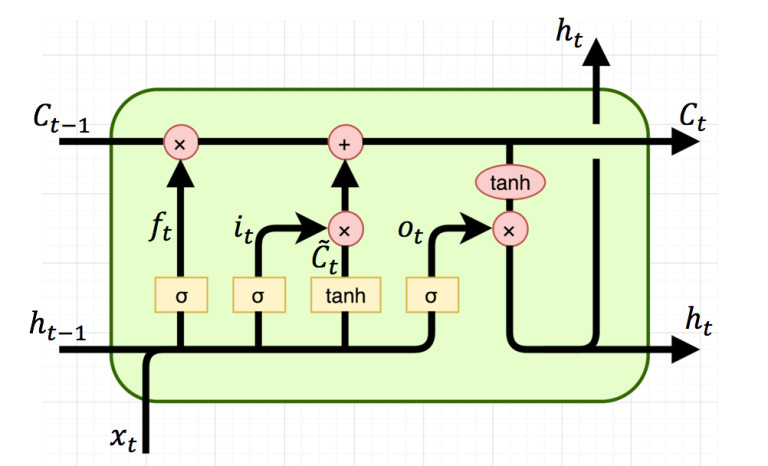
\includegraphics[width=0.7\textwidth]{Figures/lstm-all.jpg}
	\caption[Mô hình LSTM.]{Mô hình LSTM.}
	\label{fig:lstm-all.jpg} 
\end{figure}
LSTM được thiết kế để tránh được vấn đề phụ thuộc xa (long-term dependency). Việc nhớ thông tin trong suốt thời gian dài là đặc tính mặc định của chúng, chứ ta không cần phải huấn luyện nó để có thể nhớ được. Tức là ngay nội tại của nó đã có thể ghi nhớ được mà không cần bất kì can thiệp nào.

Mọi mạng hồi quy đều có dạng là một chuỗi các mô-đun lặp đi lặp lại của mạng nơ-ron. Với mạng RNN chuẩn, các mô-dun này có cấu trúc rất đơn giản, thường là một tầng tanh
\begin{figure}[h!]
	\centering
	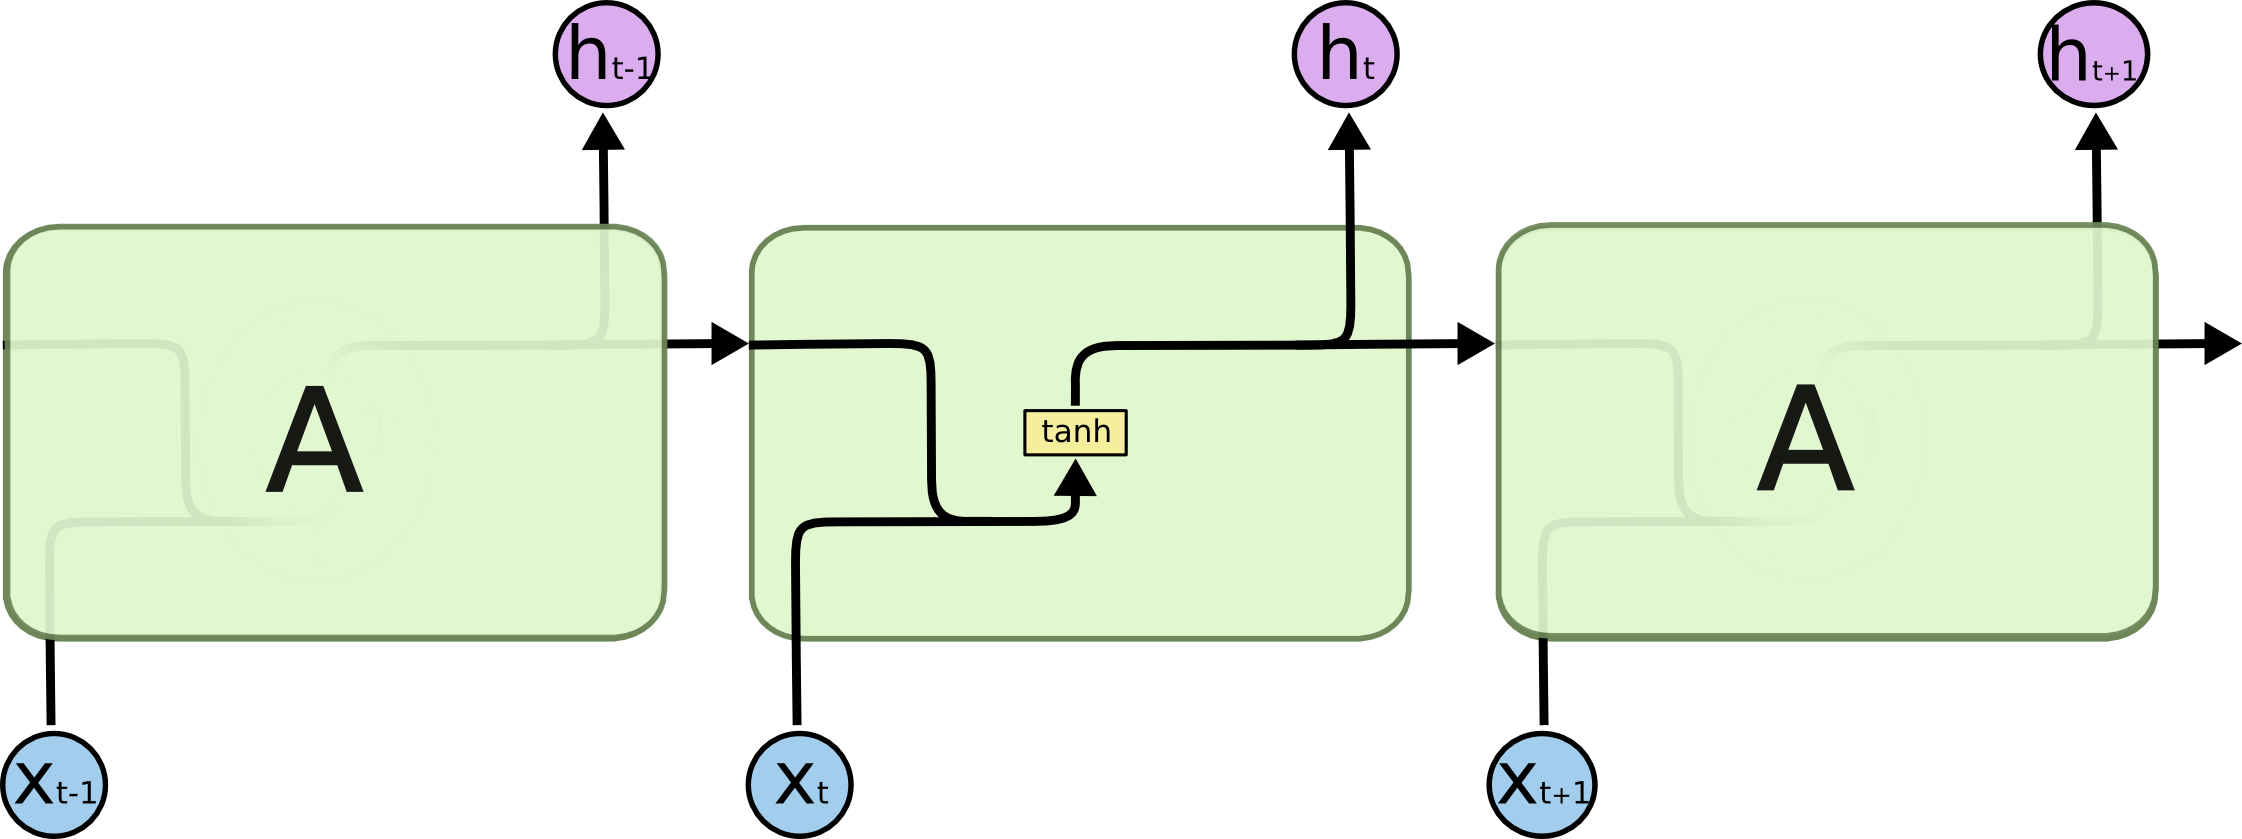
\includegraphics[width=0.7\textwidth]{LSTM3-SimpleRNN.png}
	\caption[Mạng RNN chuẩn.]{Mạng RNN chuẩn.}
	\label{fig:LSTM3-SimpleRNN.png} 
\end{figure}
LSTM cũng có kiến trúc dạng chuỗi như vậy, nhưng các mô-đun trong nó có cấu trúc khác với mạng RNN chuẩn. Thay vì chỉ có một tầng mạng nơ-ron, chúng có tới 4 tầng tương tác với nhau một cách rất đặc biệt.

\begin{figure}[h!]
	\centering
	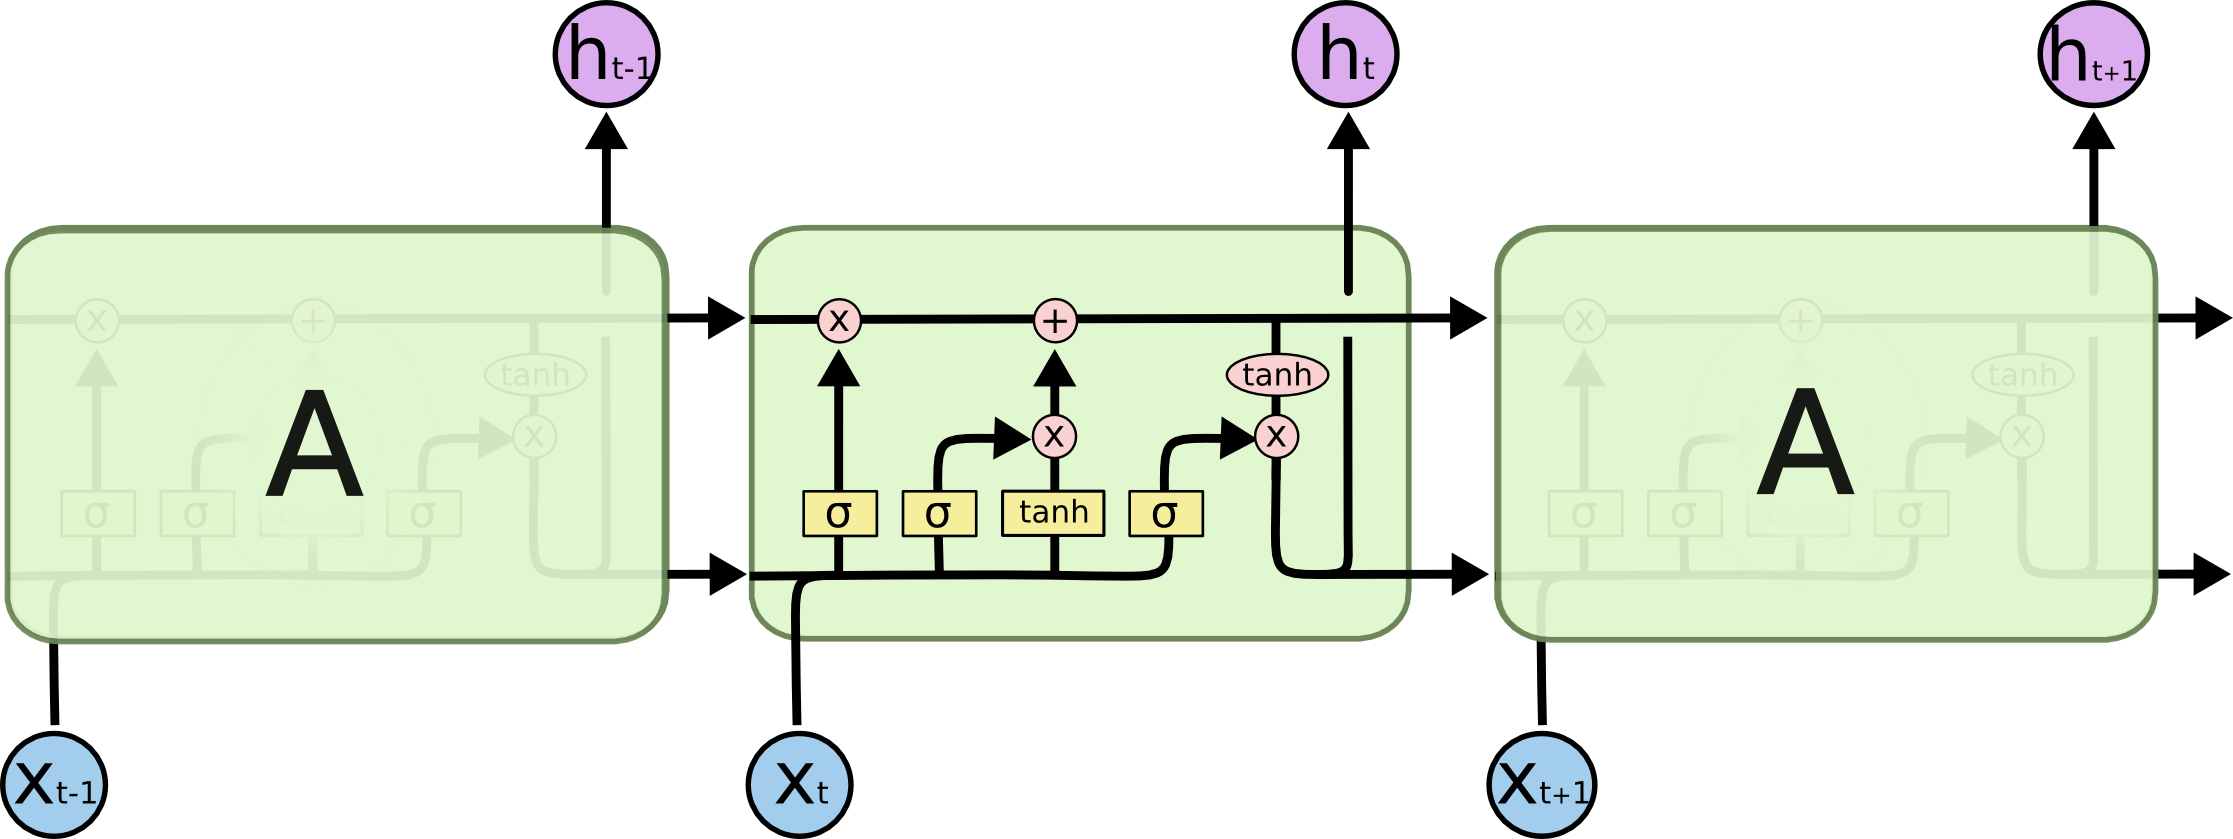
\includegraphics[width=0.7\textwidth]{Figures/LSTM3-chain.png}
	\caption[Mạng LSTM.]{Mạng LSTM.}
	\label{fig:LSTM.png} 
\end{figure}
\subsubsection{Ý tưởng cốt lõi của LSTM}
Chìa khóa của LSTM là trạng thái tế bào (cell state) - chính đường chạy thông ngang phía trên của sơ đồ hình vẽ.

Trạng thái tế bào là một dạng giống như băng truyền. Nó chạy xuyên suốt tất cả các mắt xích (các nút mạng) và chỉ tương tác tuyến tính đôi chút. Vì vậy mà các thông tin có thể dễ dàng truyền đi thông suốt mà không sợ bị thay đổi.

\begin{figure}[h!]
	\centering
	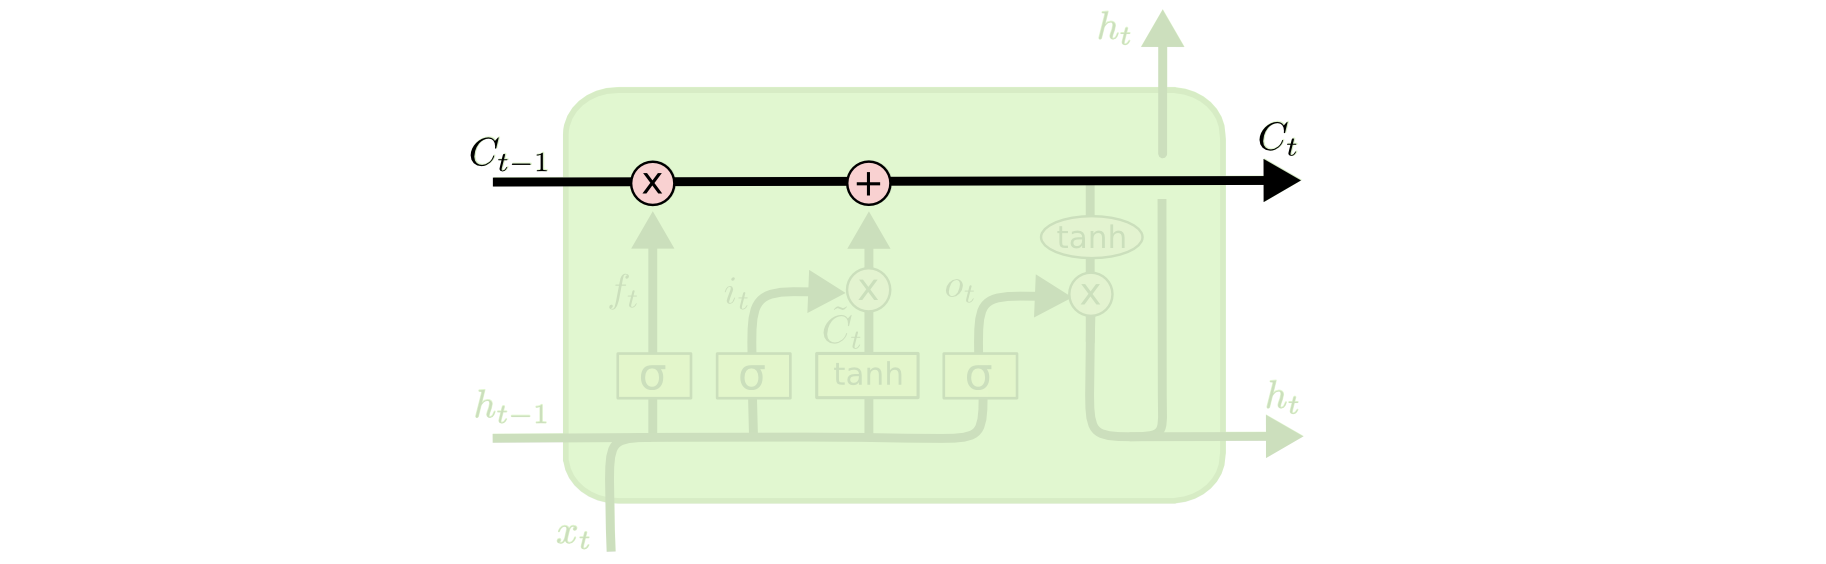
\includegraphics[width=0.7\textwidth]{Figures/LSTM3-C-line.png}
	\caption[Mạng LSTM line.]{Mạng LSTM line.}
	\label{fig:LSTM3-C-line.png} 
\end{figure}
LSTM có khả năng bỏ đi hoặc thêm vào các thông tin cần thiết cho trạng thái tế báo, chúng được điều chỉnh cẩn thận bởi các nhóm được gọi là cổng (gate).

Các cổng là nơi sàng lọc thông tin đi qua nó, chúng được kết hợp bởi một tầng mạng sigmoid và một phép nhân.

\begin{figure}[h!]
	\centering
	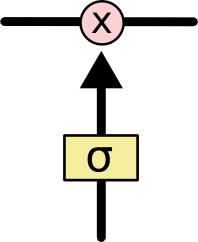
\includegraphics[width=0.7\textwidth]{Figures/LSTM3-gate.png}
	\caption[Cổng Gate.]{Cổng Gate.}
	\label{fig:LSTM3-gate.png} 
\end{figure}
Tầng sigmoid sẽ cho đầu ra là một số trong khoản [0,1], mô tả có bao nhiêu thông tin có thể được thông qua. Khi đầu ra là 0 thì có nghĩa là không cho thông tin nào qua cả, còn khi là 1 thì có nghĩa là cho tất cả các thông tin đi qua nó.
Một LSTM gồm có 3 cổng như vậy để duy trì và điều hành trạng thái của tế bào.
\subsubsection{Thành phần của LSTM}


\subsubsection{Bên trong LSTM}

\begin{itemize}
    \item Bước đầu tiên của LSTM là quyết định xem thông tin nào cần bỏ đi từ trạng thái tế bào. Quyết định này được đưa ra bởi tầng sigmoid - gọi là “tầng cổng quên” (forget gate layer) . Nó sẽ lấy đầu vào là  \( h_{t-1} \) và \( x_{t} \) rồi đưa kết quả là một trong khoảng [0,1] cho mỗi trạng thái tế bào \( C_{t-1} \) . Đầu ra là 1 thể hiện rằng nó giữ toàn bộ thông tin lại . còn 0 chỉ là toàn bộ thông tin sẽ bị bỏ đi 
    \begin{figure}[h!]
	\centering
	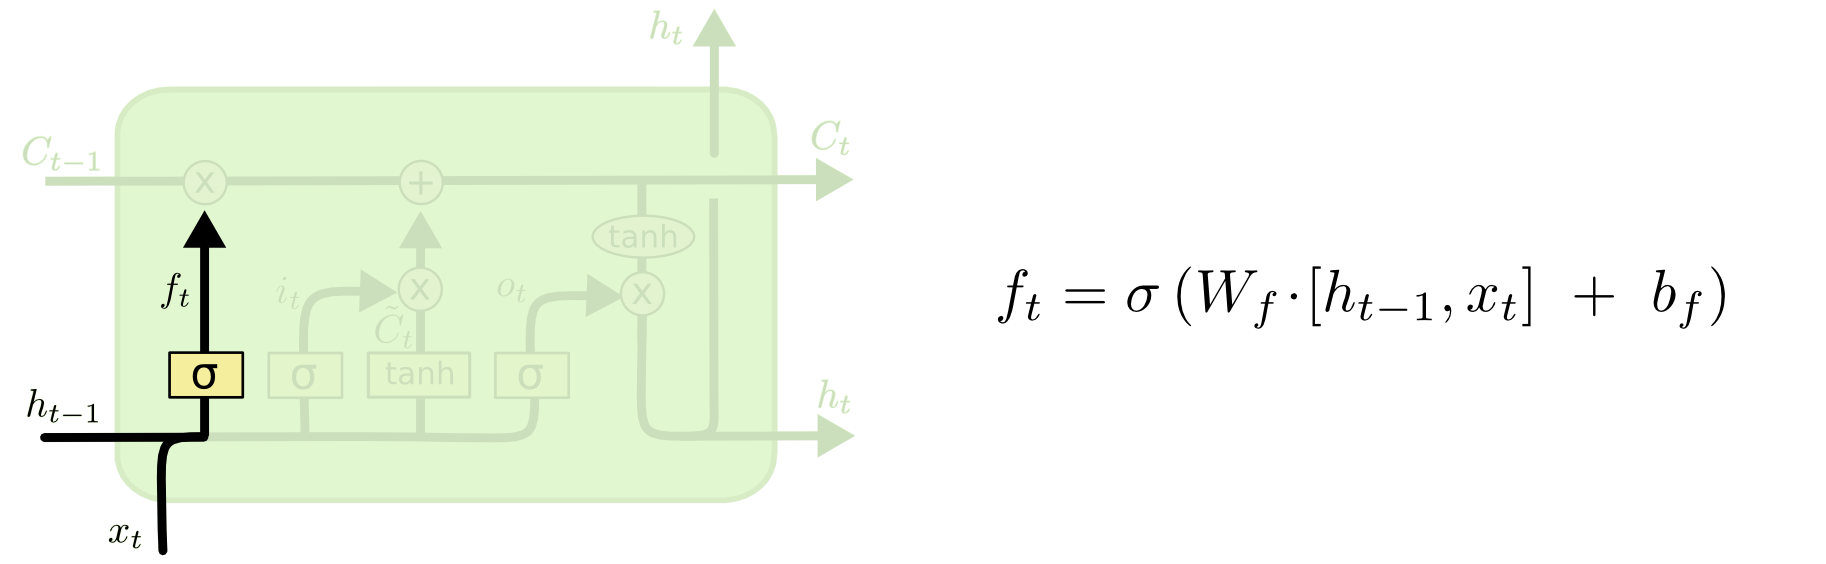
\includegraphics[width=0.7\textwidth]{Figures/LSTM3-focus-f.png}
	\caption[Forget Gate.]{Forget Gate.}
	\label{LSTM3-focus-f.png} 
\end{figure}
    \item Bước tiếp theo là quyết định xem thông tin mới nào ta sẽ lưu vào trạng thái tế bào. Việc này gồm 2 phần. Đầu tiên là sử dụng một tầng sigmoid được gọi là “tầng cổng vào” (input gate layer) để quyết định giá trị nào ta sẽ cập nhập. Tiếp theo là một tầng tanh để tạo ra một vec-to cho giá trị mới \( C_{t} \) nhằm thêm vào cho trạng thái. Trong bước tiếp theo, ta sẽ kết hợp 2 giá trị đó lại để tạo ra một cập nhập cho trạng thái.
    \begin{figure}[h!]
	\centering
	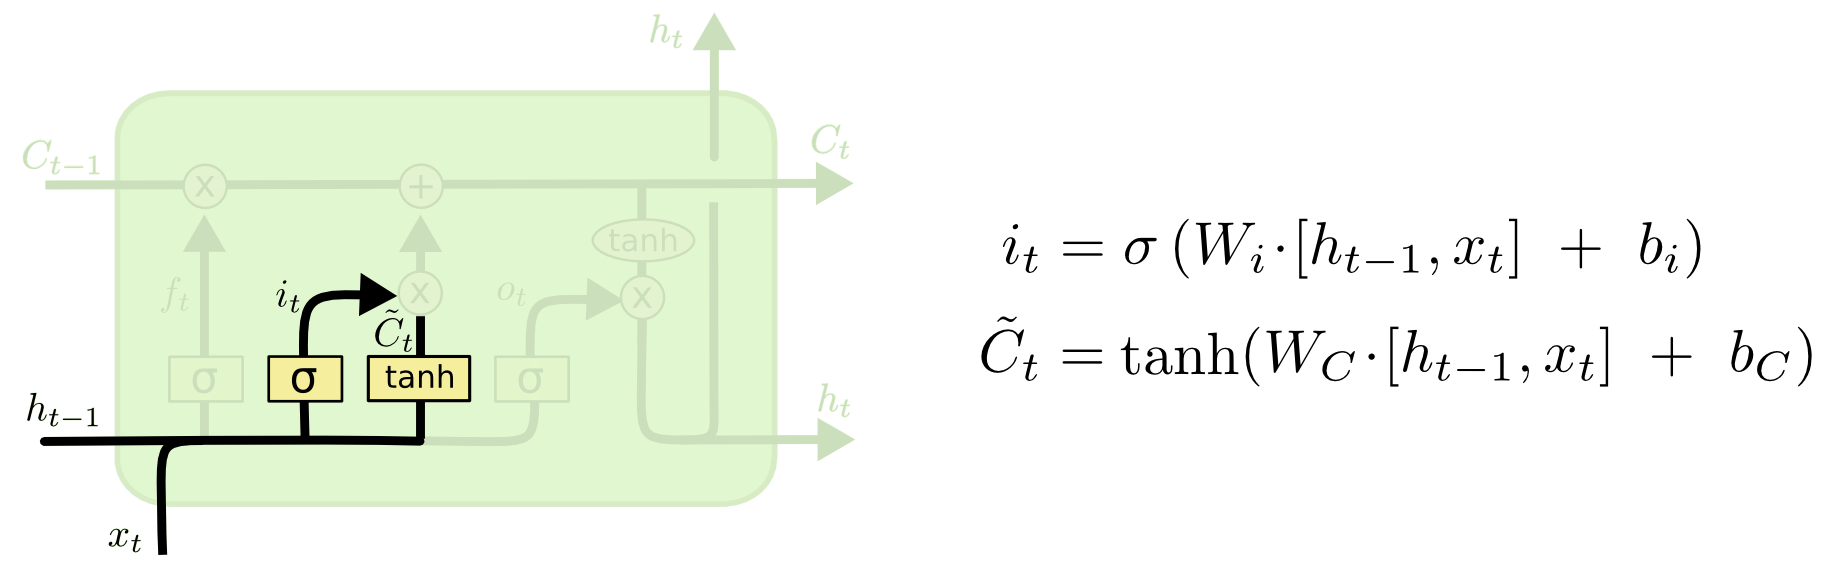
\includegraphics[width=0.7\textwidth]{Figures/LSTM3-focus-i.png}
	\caption[Input Gate.]{Input Gate.}
	\label{LSTM3-focus-i.png} 
\end{figure}
    \item Sau đó , LSTM cập nhật trạng thái của Cell State \( C_{t-1} \) thành trạng thái mới \( C_{t} \) bằng cách kết hợp thông tin mới và thông tin cũ . Ta sẽ nhân trạng thái cũ với \( f_{t} \) để bỏ đi những thông tin ta quyết định quên lúc trước. Sau đó cộng thêm \( i_{t} \) * \( C_{t} \)  Trạng thái mơi thu được này phụ thuộc vào việc ta quyết định cập nhập mỗi giá trị trạng thái ra sao.
    \begin{figure}[h!]
	\centering
	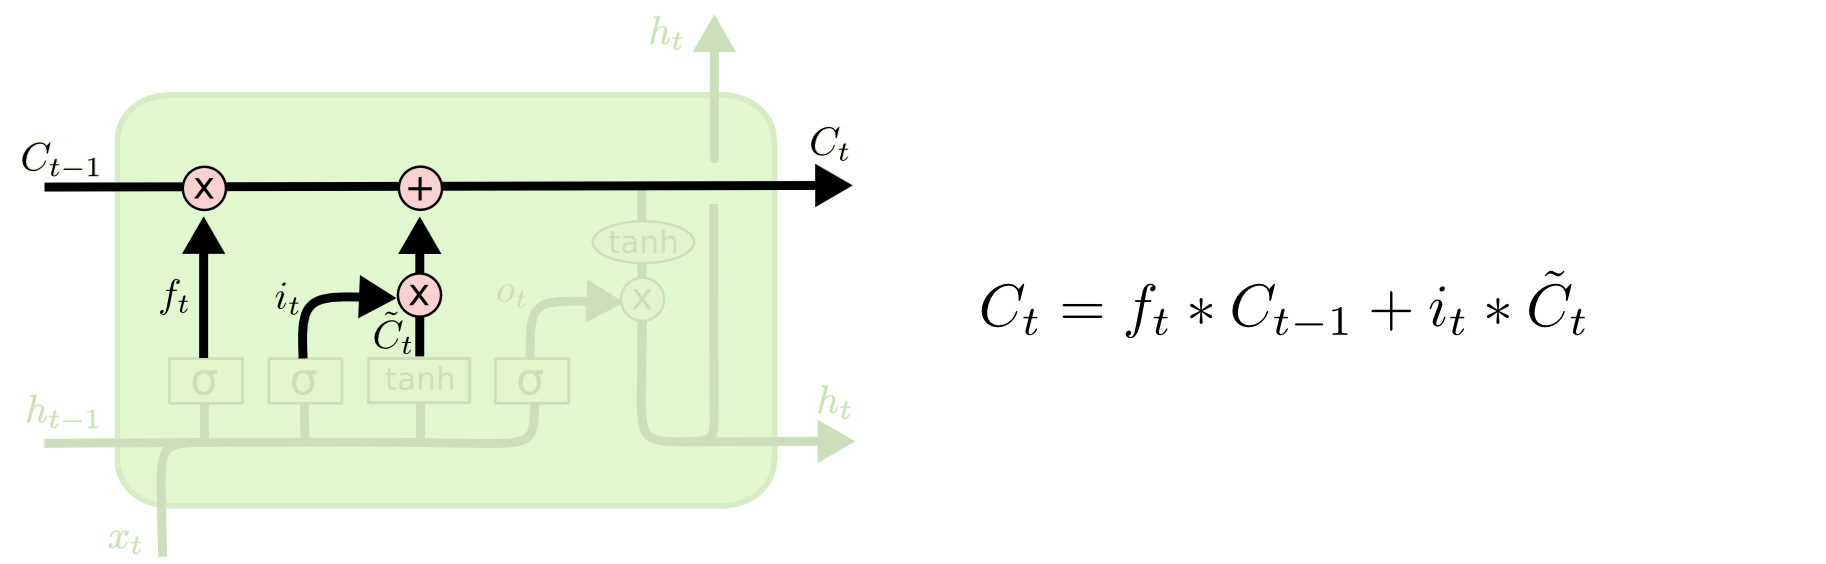
\includegraphics[width=0.7\textwidth]{Figures/LSTM3-focus-C.png}
	\caption[Cell Gate.]{Cell Gate.}
	\label{LSTM3-focus-C.png} 
\end{figure}
    \item Cuối cùng ,LSTM tính toán giá trị của cổng đầu ra và sử dụng nó để tính toán đầu ra của đơn vị LSTM hiện tại và truyền trạng thái ẩn tới đơn vị LSTM tiếp theo trong chuỗi .Đầu tiên, ta chạy một tầng sigmoid để quyết định phần nào của trạng thái tế bào ta muốn xuất ra. Sau đó, ta đưa nó trạng thái tế bảo qua một hàm tanh để co giá trị nó về khoảng [-1,1],và nhân nó với đầu ra của cổng sigmoid để được giá trị đầu ra ta mong muốn.
    \begin{figure}[h!]
	\centering
	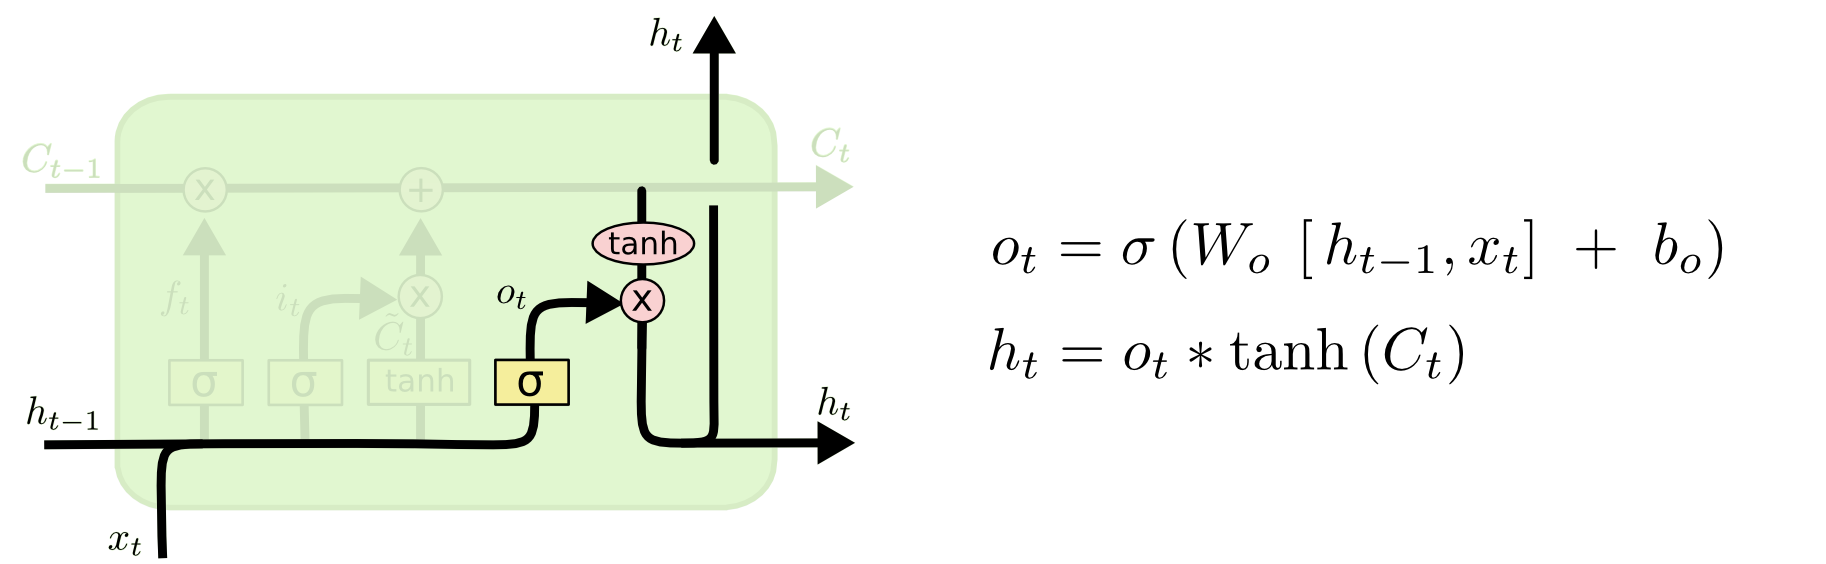
\includegraphics[width=0.7\textwidth]{Figures/LSTM3-focus-o.png}
	\caption[Output Gate.]{Output Gate.}
	\label{LSTM3-focus-C.png} 
\end{figure}
\end{itemize}
\subsubsection{Ưu điểm của LSTM}
LSTM là một bước lớn trong việc sử dụng RNN. Ý tưởng của nó giúp cho tất cả các bước của RNN có thể truy vấn được thông tin từ một tập thông tin lớn hơn. Ví dụ, nếu bạn sử dụng RNN để tạo mô tả cho một bức ảnh, nó có thể lấy một phần ảnh để dự đoán mô tả từ tất cả các từ đầu vào. Bằng chứng là Xu, et al. (2015) đã thực hiện được chính xác việc này. Hiện nay cũng đã có nhiều kết qua thực sự rất thú vị được chú ý và dường như có nhiều kết quả hơn chúng ta vẫn biết.
LSTM có những ưu điểm quan trọng áp dụng vào bài toán nhận diện hành động con người và xử lý chuỗi thời gian 
\begin{itemize}
    \item LSTM có khả năng lưu trữ thông tin lâu dài và xử lý các chuỗi dữ liệu dài và phức tạp hơn so với các kiến trúc mạng nơ-ron tái phát khác như mạng Elman hay mạng Jordan.
    \item LSTM được sử dụng để giải quyết các vấn đề trong xử lý ngôn ngữ tự nhiên như: phân loại văn bản, dịch máy, sinh văn bản tự động, tổng hợp giọng nói, và xử lý dữ liệu ngôn ngữ tự nhiên khác.
    \item LSTM có thể được sử dụng để giải quyết các vấn đề trong xử lý âm thanh và hình ảnh như: nhận dạng giọng nói dạng (voice recognition), phân loại hình ảnh, nhận diện khuôn mặt, phát hiện đối tượng và các ứng dụng khác trong lĩnh vực thị giác máy tính.
\end{itemize}

\section{Các thư viện sử dụng}
\subsubsection{Thư viện Numpy}
Thư viện NumPy (Numerical Python) là một thư viện Python phổ biến được sử dụng để làm việc với mảng đa chiều và các phép toán số học trên chúng. NumPy cung cấp một cấu trúc dữ liệu mảng mạnh mẽ và các hàm tiện ích để thực hiện các phép toán số học, xử lý mảng và thao tác trên dữ liệu số.
Dưới đây là một số khái niệm và tính năng chính của NumPy:
\begin{itemize}
	\item Mảng NumPy (ndarray): Mảng NumPy là cấu trúc dữ liệu chính trong NumPy, cho phép lưu trữ và xử lý các mảng đa chiều. Mảng NumPy có kích thước cố định và các phần tử trong mảng cùng kiểu dữ liệu.
	
	\item Các phép toán số học: NumPy cung cấp các hàm và toán tử cho phép thực hiện các phép toán số học trên mảng như cộng, trừ, nhân, chia, lũy thừa, căn bậc hai, logarit...
	
	\item Truy cập phần tử: Bạn có thể truy cập và thay đổi giá trị các phần tử trong mảng NumPy bằng cách sử dụng chỉ mục và cắt mảng (slicing).
	
	\item Hàm toán học và thống kê: NumPy cung cấp nhiều hàm toán học và thống kê tiện ích như min, max, mean, sum, std,... để thao tác trên mảng.
	
	\item Hàm điều kiện: NumPy cung cấp các hàm và phương thức cho phép kiểm tra và lựa chọn các phần tử trong mảng dựa trên các điều kiện như np.where, np.logical$\_$and, np.logical$\_$or,...
	
	\item Thao tác trên mảng: NumPy cung cấp các hàm và phương thức để thực hiện các phép biến đổi mảng như reshape, transpose, flatten, concatenate,...
	
	\item Tích hợp C/C++: NumPy cho phép tích hợp mã C/C++ vào mã Python thông qua giao diện C API của nó, giúp tăng tốc độ xử lý các phép toán số học.
	
	\item NumPy được sử dụng rộng rãi trong nhiều lĩnh vực như khoa học dữ liệu, máy học, tính toán khoa học, xử lý ảnh và âm thanh, mô phỏng vật lý,... Thư viện này là một phần quan trọng của hệ sinh thái Python cho tính toán số và xử lý dữ liệu.
\end{itemize}

\subsubsection{Thư viện OpenCV}

Thư viện cv2 (OpenCV) là một thư viện mã nguồn mở được sử dụng rộng rãi trong xử lý ảnh và thị giác máy tính trong ngôn ngữ lập trình Python. OpenCV cung cấp nhiều chức năng và công cụ mạnh mẽ để xử lý, phân tích và trực quan hóa ảnh và video. Dưới đây là một số chức năng chính của thư viện cv2:

\begin{itemize}
	\item Đọc và ghi ảnh và video: OpenCV cung cấp các hàm để đọc và ghi các tệp tin ảnh và video từ các nguồn khác nhau, bao gồm ổ đĩa, camera,...
	
	\item Xử lý ảnh: OpenCV cung cấp nhiều chức năng để xử lý ảnh, bao gồm chuyển đổi màu sắc, cắt, xoay, thu phóng, lật, v.v. Bạn cũng có thể áp dụng các bộ lọc, làm mờ, lọc nhiễu, phát hiện cạnh và nhiều phép biến đổi khác cho ảnh.
	
	\item Xử lý video: OpenCV hỗ trợ xử lý video, bao gồm khung hình theo thời gian, trích xuất khung hình, ghi lại video và áp dụng các hiệu ứng video.
	
	\item Xử lý thị giác máy tính: OpenCV cung cấp các chức năng và thuật toán để phân tích và nhận dạng các đối tượng trong ảnh, bao gồm nhận dạng khuôn mặt, phát hiện vật thể, trích xuất đặc trưng, theo dõi đối tượng,...
	
	\item Xử lý điểm ảnh: OpenCV cho phép bạn truy cập và chỉnh sửa các điểm ảnh trực tiếp, bao gồm xử lý pixel, tạo hiệu ứng đồ họa và thực hiện các phép tính điểm ảnh phức tạp.
	
	\item Hiển thị ảnh: OpenCV cung cấp các chức năng để hiển thị ảnh và video trực tiếp trên màn hình, tạo cửa sổ đồ họa và tương tác với ảnh.
\end{itemize}

Thư viện cv2 có tính ổn định, tốc độ xử lý nhanh và rất phổ biến trong cộng đồng xử lý ảnh và thị giác máy tính.

\subsubsection{Thư viện Tensorflow}

Thư viện TensorFlow là một thư viện mã nguồn mở phát triển bởi Google AI và được sử dụng rộng rãi trong lĩnh vực học máy và trí tuệ nhân tạo. TensorFlow cung cấp một cấu trúc dữ liệu gọi là "đồ thị tính toán" (computational graph) để biểu diễn và thực thi các phép tính toán số trên dữ liệu. Đồ thị tính toán trong TensorFlow bao gồm các nút (nodes) đại diện cho các phép tính toán và các cung (edges) đại diện cho luồng dữ liệu giữa các nút. Dưới đây là một số khái niệm và tính năng chính của TensorFlow:

\begin{itemize}
	\item Đồ thị tính toán (Computational graph): TensorFlow sử dụng đồ thị tính toán để biểu diễn và thực thi các phép tính toán. Đồ thị tính toán giúp tối ưu hóa và tận dụng được tính song song của phần cứng để thực hiện các phép tính nhanh chóng.
	
	\item Tensors: TensorFlow sử dụng cấu trúc dữ liệu tensor để lưu trữ và xử lý dữ liệu. Tensor có thể là một vector, ma trận, hay một mảng đa chiều với các phần tử cùng kiểu dữ liệu.
	
	\item Các lớp và phép tính: TensorFlow cung cấp một loạt các lớp và phép tính để xây dựng các mô hình học máy. Các lớp bao gồm các lớp mạng nơ-ron, lớp tích chập, lớp tổng hợp, lớp tái tạo,... Phép tính bao gồm các phép tính toán như cộng, trừ, nhân, chia, lũy thừa,...
	
	\item Tối ưu hóa và tạo mô hình: TensorFlow cung cấp các tối ưu hóa để tối đa hóa hiệu suất và tăng tốc độ huấn luyện mô hình. Ngoài ra, TensorFlow cũng cung cấp khả năng tạo và lưu trữ các mô hình đã huấn luyện để sử dụng sau này.
	
	\item Tích hợp và mở rộng: TensorFlow cho phép tích hợp và mở rộng với các công cụ và thư viện khác như Keras, scikit-learn, OpenCV, v.v. Điều này giúp thực hiện các tác vụ phức tạp và kết hợp các công cụ và thuật toán khác nhau.
	
	\item Tính tương thích và di động: TensorFlow hỗ trợ nhiều phiên bản và cung cấp tính tương thích đa nền tảng, cho phép chạy trên các thiết bị di động, máy tính cá nhân, máy chủ, và cụm máy tính phân tán.
\end{itemize}

TensorFlow là một công cụ mạnh mẽ trong lĩnh vực học máy và trí tuệ nhân tạo, cho phép xây dựng và huấn luyện các mô hình phức tạp và giải quyết các bài toán thực tế.

\subsubsection{Thư viện Sklearn}

Scikit-learn, hay còn được gọi là sklearn, là một thư viện mã nguồn mở phổ biến trong ngôn ngữ lập trình Python được sử dụng cho Machine Learning và Data Mining. Scikit-learn cung cấp nhiều công cụ và thuật toán tiện ích để xây dựng và đánh giá các mô hình học máy, phân tích dữ liệu và thực hiện các tác vụ tiền xử lý dữ liệu. Dưới đây là một số chức năng và tính năng chính của thư viện scikit-learn:

\begin{itemize}
	\item Cung cấp các thuật toán học máy tiêu chuẩn: Scikit-learn cung cấp các thuật toán học máy phổ biến như hồi quy tuyến tính, hồi quy logistic, máy vector hỗ trợ (SVM), cây quyết định, Random Forest, K-means clustering,... Các thuật toán này được triển khai một cách hiệu quả và dễ sử dụng.
	
	\item Tích hợp các công cụ tiền xử lý dữ liệu: Scikit-learn cung cấp nhiều công cụ tiền xử lý dữ liệu như chuẩn hóa dữ liệu, mã hóa biến định danh, xử lý giá trị thiếu, trích xuất đặc trưng,... Điều này giúp chuẩn bị dữ liệu cho việc huấn luyện mô hình.
	
	\item Đánh giá và tối ưu hóa mô hình: Scikit-learn cung cấp các phép đo và công cụ để đánh giá hiệu suất của mô hình học máy, bao gồm chia dữ liệu thành tập huấn luyện và tập kiểm tra, cross-validation, tính toán độ chính xác, độ phân loại, mất mát,... Ngoài ra, scikit-learn cũng cung cấp các công cụ tối ưu hóa để điều chỉnh các siêu tham số của mô hình.
	
	\item Tích hợp với các thư viện khác: Scikit-learn tích hợp tốt với các thư viện khác trong hệ sinh thái của Python như NumPy, Pandas và Matplotlib, tạo điều kiện thuận lợi cho xử lý dữ liệu và trực quan hóa kết quả.
\end{itemize}

Scikit-learn là một công cụ mạnh mẽ và phổ biến trong lĩnh vực Machine Learning, đặc biệt là trong các tác vụ phân loại, hồi quy và gom cụm dữ liệu. Với tư cách là một thư viện mã nguồn mở, scikit-learn đang tiếp tục được phát triển và cung cấp cập nhật mới để phục vụ cộng đồng Machine Learning ngày càng lớn.

\subsubsection{Thư viện Matplotlib}

Matplotlib là một thư viện trong Python được sử dụng để tạo và hiển thị đồ thị, biểu đồ, hình ảnh và các loại visualizations khác. Nó cung cấp các công cụ mạnh mẽ để tạo ra các biểu đồ chất lượng cao, giúp bạn trực quan hóa dữ liệu một cách dễ dàng và linh hoạt. Dưới đây là một số thành phần chính trong thư viện matplotlib:

\begin{itemize}
	\item pyplot: Giao diện API cơ bản của Matplotlib, cung cấp các hàm để tạo và tùy chỉnh đồ thị và biểu đồ.
	
	\item Figure: Đại diện cho một hình ảnh hoặc một tệp tin hình ảnh.
	
	\item Axes: Cung cấp các phương thức để tạo các đối tượng đồ thị như các trục, điểm, đường.
	
	\item Subplots: Cho phép tạo và quản lý nhiều đồ thị trong cùng một hình ảnh.
	
	\item Plot: Hàm để tạo các loại đồ thị và biểu đồ, bao gồm đồ thị đường (line plot), biểu đồ cột (bar plot), biểu đồ hộp (box plot), đồ thị điểm (scatter plot).
	
	\item Colorbar: Hiển thị thanh màu để giải thích giá trị của màu sắc trong đồ thị.
	
	\item Title, Label, Legend`: Cung cấp các phương thức để thêm tiêu đề, nhãn và chú giải vào đồ thị.
\end{itemize}

Matplotlib cũng hỗ trợ nhiều kiểu đồ thị và biểu đồ, cho phép bạn tùy chỉnh màu sắc, kích thước, kiểu đường, điểm, các đánh dấu trục, v.v. Thư viện này rất linh hoạt và mạnh mẽ, cho phép bạn tạo ra các visualizations phức tạp và tùy chỉnh chúng theo ý muốn.

\subsubsection{Thư viện Keras}

Keras là một thư viện mã nguồn mở cho Python được sử dụng để xây dựng các mô hình học máy và mạng nơ-ron. Nó được thiết kế để làm cho việc xây dựng mô hình học máy trở nên dễ dàng và nhanh chóng hơn. Keras có nhiều tính năng hữu ích, bao gồm:

\begin{itemize}
	\item Dễ dàng sử dụng: Keras được thiết kế để làm cho việc xây dựng mô hình học máy trở nên dễ dàng và trực quan hơn.
	
	\item Tích hợp với các thư viện tính toán số: Keras hỗ trợ các thư viện tính toán số như TensorFlow, Theano và CNTK, cho phép bạn chọn thư viện tính toán số phù hợp nhất cho dự án của mình.
	
	\item Hỗ trợ nhiều loại mô hình: Keras hỗ trợ nhiều loại mô hình, bao gồm mạng nơ-ron tiêu chuẩn, mạng nơ-ron tích chập và mạng nơ-ron tái tạo.
	
	\item Tích hợp với các công cụ tối ưu hóa: Keras cung cấp các công cụ tối ưu hóa để giúp bạn tìm kiếm các tham số tốt nhất cho mô hình của mình.
	
	\item Hỗ trợ các lớp và hàm kích hoạt tiêu chuẩn: Keras cung cấp các lớp và hàm kích hoạt tiêu chuẩn để giúp bạn xây dựng mô hình học máy nhanh chóng và dễ dàng.
\end{itemize}

Keras là một trong những thư viện phổ biến nhất cho việc xây dựng các mô hình học máy và mạng nơ-ron. 

\section{Thư viện MediaPipe}

Đây là một công cụ do google thiết kế ra, nó cung cấp nhiều tính năng cho các bài toán AI/ML chạy trên nhiều nền tảng khác nhau MediaPipe là tập hợp của một loạt các giải pháp Machine Learning đa nền tảng, có thể can thiệp được và cực kỳ lightweight.

Một số ưu điểm có thể kể tới của giải pháp này bao gồm:

\begin{itemize}
	\item Cung cấp một giải pháp inference nhanh chóng: Google khẳng định rằng bộ công cụ này có thể chạy ổn định trên hầu hết các cấu hình phần cứng thông dụng.
	
	\item Mã nguồn mở và miễn phí: Toàn bộ source code được công khai trên MediaPipe, người dùng hoàn toàn có thể sử dụng và tùy chỉnh trực tiếp để phù hợp với bài toán của mình.
	
	\item Dễ dàng cài đặt và triển khai: Việc cài đặt cực kỳ dễ dàng và tiện lợi, có thể triển khai trên nhiều nền tảng khác nhau như Mobile (Android/iOS), Desktop/Cloud, Web và IoT devices.
\end{itemize}

Hầu hết các bài toán nổi bật trong lĩnh vực Computer Vision - Thị giác máy tính, đều được Google cài đặt trong MediaPipe. Trong bài toán mình sẽ sử dụng Human Pose Estimation Mở rộng từ bài toán Hands Detection, Human Pose Estimation cung cấp một mô hình skeleton 3D cho cả cơ thể, với các khớp quan trọng được định nghĩa sẵn và được nối với nhau để tạo thành khung của người. Chiến thuật được đặt ra cho bài toán này tương tự như bài Hands Detection và Face Mesh. BlazeFace, một lần nữa, được sử dụng làm tư tưởng chính cho thuật toán xử lý bài này.

Các ứng dụng của mediapipe
\begin{itemize}
    \item Phát hiện khuôn mặt
    \item Tìm lưới khuôn mặt: dùng cho các ứng dụng biến đổi khuôn mặt như Tiktok
    \item Iris: tìm khoảng cách từ đồng tử của mắt đến camera mà không cần Depth webcam
    \item Detect cử chỉ bàn tay
    \item Tìm hình dáng của cơ thể
    \item Object detection , Box tracking
    \item Theo dõi chuyển động của vật thể
\end{itemize}

\section{Chỉ số đánh giá hiệu suất}

Để đánh giá phân loại ảnh được chính xác, các mô hình trong phần trước sữ được chạy bằng cách sử dụng bộ dữ liệu dưới dạng hình ảnh, vì vậy cần có sự điều chỉnh để nâng cấp độ chính xác của chúng. Đối với mỗi mô hình 3 kết quả điển hình được hiển thị trong CNN là:

\begin{itemize}
	\item Đồ thị độ chính xác (model ACC): ACC cho biết sự thay đổi độ chính xác của mô hình qua các vòng lặp/epochs trong quá trình huấn luyện.
	
	\item Đồ thị loss (model loss): Đồ thị loss biểu thị sự thay đổi của hàm loss của mô hình qua các vòng lặp hoặc epochs trong quá trình huấn luyện. Hàm loss tính toán sự sai khác giữa giá trị dự đoán của mô hình và giá trị thực tế.
	
	\item Confusion matrix: Về cơ bản, Confusion matrix thể hiện có bao nhiêu điểm dữ liệu thực sự thuộc vào một class, và được dự đoán là rơi vào một class. 
	
	\begin{figure}[h!]
		\centering
		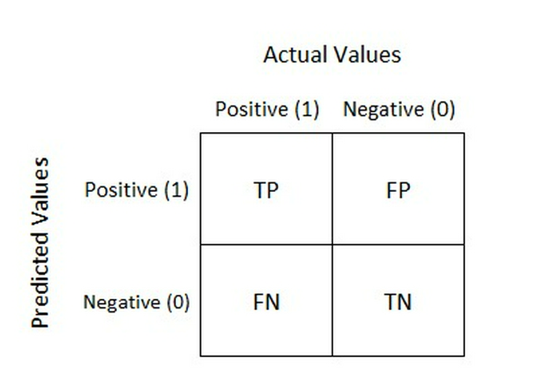
\includegraphics[width=0.7\textwidth]{cofusion.png}
		\caption[Confusion matrix.]{Confusion matrix.}
		\label{fig:cm} 
	\end{figure}

	\begin{itemize}
		\item TP (True Positive): Số lượng dự đoán chính xác.
		
		\item TN (True Negative): Số lương dự đoán chính xác một cách gián tiếp. Là khi mô hình dự đoán đúng một người không bị bệnh tức là việc không chọn trường hợp bị bệnh là chính xác.
		
		\item FP (False Positive - Type 1 Error): Số lượng các dự đoán sai lệch. Là khi mô hình dự đoán một người bị bệnh và người đó hoàn toàn khỏe mạnh.
		
		\item FN (False Negative - Type 2 Error): Số lượng các dự đoán sai lệch một cách gián tiếp. Là khi mô hình dự đoán một người không bị bệnh nhưng người đó bị bệnh, tức là việc không chọn trường hợp bị bệnh là sai. 		
	\end{itemize}
	$\Longrightarrow$ Từ 4 chỉ số TP, TN, FP, FN, ta có 4 chỉ số để đánh giá mức độ tin cậy của một mô hình:
\end{itemize}

\begin{itemize}
	\item Accuracy: Được tính bằng cách chia tổng số dự đoán đúng cho tất cả các dự đoán.
	
	\begin{figure}[h!]
		\centering
		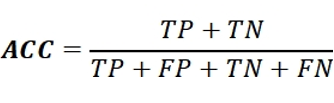
\includegraphics[width=0.45\textwidth]{acc1.png}
		\caption[Accuracy.]{Accuracy.}
		\label{fig:acc} 
	\end{figure}
		
	\item Precision: Trong tất cả các dự đoán Positive được đưa ra, bao nhiêu dự đoán là chính xác.
	
	\begin{figure}[h!]
		\centering
		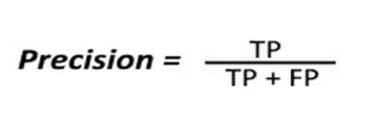
\includegraphics[width=0.6\textwidth]{precision.png}
		\caption[Precision.]{Precision.}
		\label{fig:precision} 
	\end{figure}
	
	\item Recall: Trong tất cả các trường hợp Positive, bao nhiêu trường hợp đã được dự đoán chính xác.		
	
	\begin{figure}[h!]
		\centering
		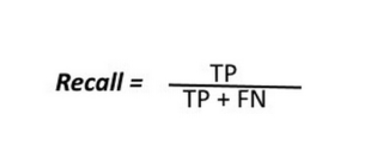
\includegraphics[width=0.6\textwidth]{recall.png}
		\caption[Recall.]{Recall.}
		\label{fig:recall} 
	\end{figure}

	\item F1-Score: Dùng để đánh giá mức độ tin cậy chung của mô hình
	
	\begin{figure}[h!]
		\centering
		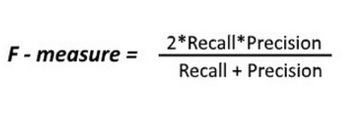
\includegraphics[width=0.6\textwidth]{score.png}
		\caption[F1-Score.]{F1-Score.}
		\label{fig:score} 
	\end{figure}
\end{itemize}








 
% Chương 3

\chapter{HUMAN ACTIVITY RECOGNITION} 

\label{Chapter3} 
Bài toán của chúng ta xây dựng đó là bài toán nhận dạng các hành động con người qua webcam hoặc video. Các hành động con người thì rất nhiều vì vậy trong bài viết này mình chỉ nhận dạng một vài hành động thường ngày qua con người. Thuật toán chúng tôi xử dụng trong bài này là CNN và mạng LSTM kết hợp với công cụ MediaPipe . Chúng tôi sẽ tiếp cận để xây dựng mô hình nhận biết theo 3 hướng :
\begin{itemize}
    \item Sử dụng công cụ MediaPipe và xây dựng mạng LSTM
    \item Xây dựng mô hình ConvLSTM
    \item Xây dựng mô hình LRCN
\end{itemize}

\section{Sử dụng công cụ MediaPipe và mạng LSTM}
    \begin{figure}[h!]
	\centering
	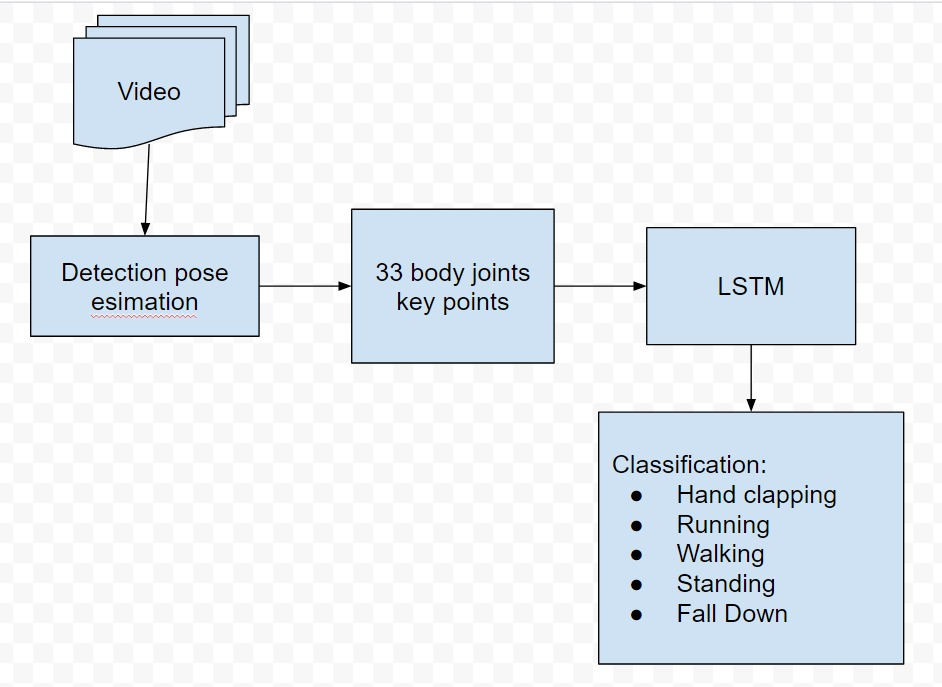
\includegraphics[width=0.7\textwidth]{Figures/luongbaitoan.jpeg}
	\caption[Luồng bài toán .]{Luồng bài toán.}
	\label{luongbaitoan.jpeg} 
    \end{figure}

\subsection{Tiền xử lý dữ liệu }
Tiền xử lý dữ liệu là một bước rất quan trọng trong việc giải quyết bất kỳ vấn đề nào trong lĩnh vực học máy. Hầu hết các bộ dữ liệu được sử dụng trong các vấn đề liên quan đến học máy cần được xử lý, làm sạch và biến đổi trước khi một thuật toán có thể được huấn luyện trên những bộ dữ liệu này.
\subsubsection{Thu thập dữ liệu }

    \begin{figure}[h!]
	\centering
	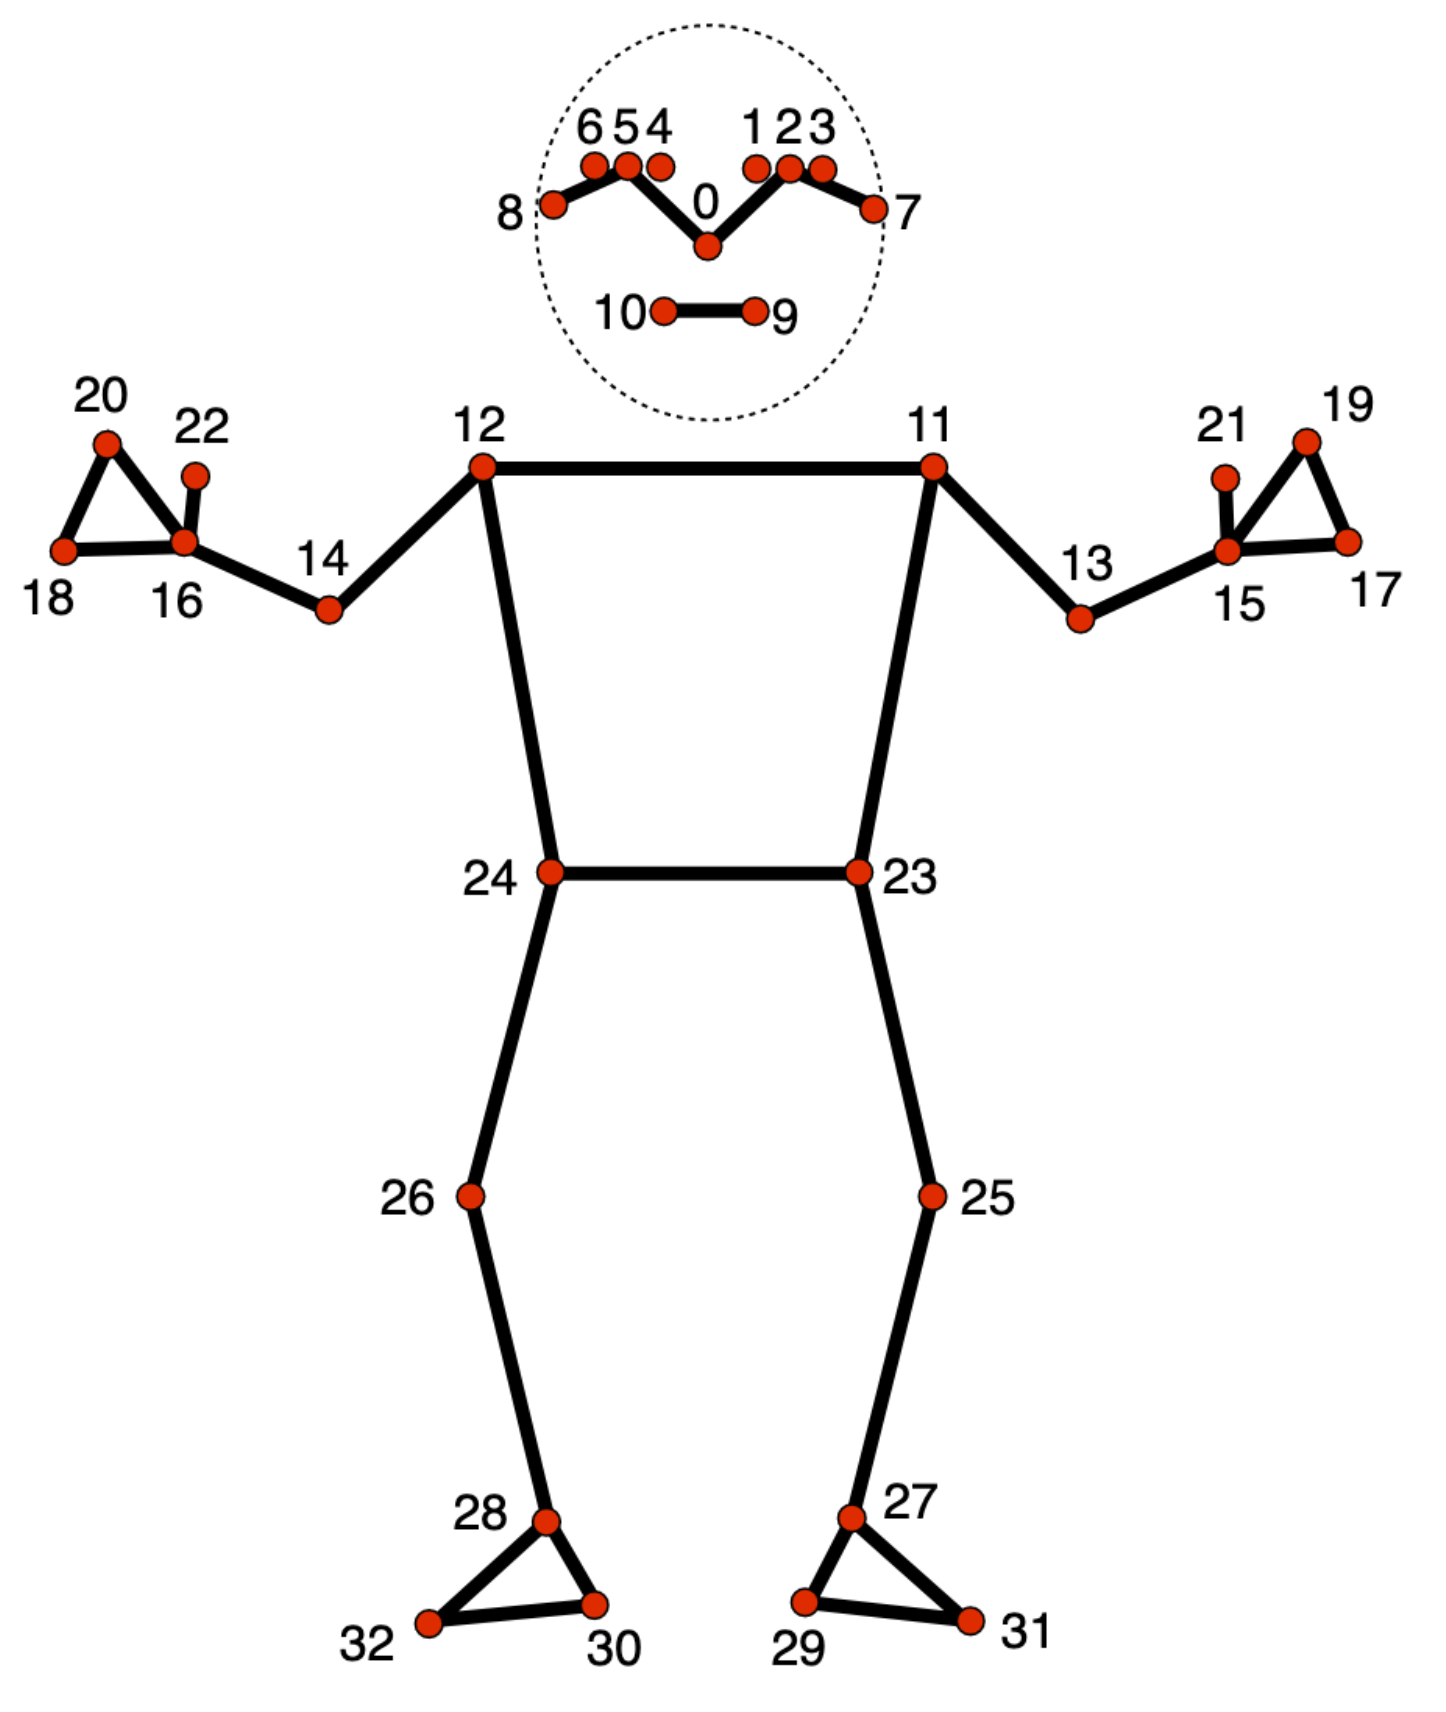
\includegraphics[width=0.7\textwidth]{Figures/pose_landmarks_index.png}
	\caption[MediaPipe Pose .]{MediaPipe Pose .}
	\label{pose_landmarks_index.png} 
    \end{figure}
Trước khi chuẩn bị dữ liệu cho đầu vào tôi sẽ giới thiệu về một công cụ mạnh mẽ \href{https://developers.google.com/mediapipe/solutions/vision/pose_landmarker/}{MediaPipe Pose} Mediapipe Pose để biết cách vẽ các điểm keypoints và cách hoạt động của nó như thế nào . Mỗi vị trí trong 33 keypoints đó đều có 4 điểm tương ứng hoặc có thể nói là tọa độ tương ứng đó là: X,Y,Z,VISIBILITY. Phần này chính là input của mạng LSTM. Chúng ta sẽ đưa 4 điểm tương ứng này với từng điểm keypoints(có 33 điểm) sẽ tao thành array, sau đó chúng ta làm phẳng nó ra 33*4 sẽ là 132 điểm. Thêm 1 vấn đề nữa là nếu như trong 1 khung hình mà không thể hết được 33 điểm thì các vị trí không thể vẽ được được gán bằng 0 hoặc xấp xỉ không nếu không nhìn rõ . 
Đầu tiên cần khởi tạo thư viện mediapipe . 

\begin{lstlisting}[style=codePython]
 	import cv2
import mediapipe as mp
import pandas as pd

cap = cv2.VideoCapture(0)

mpPose = mp.solutions.pose
pose = mpPose.Pose()
mpDraw = mp.solutions.drawing_utils
\end{lstlisting}

Bây giờ sử dụng thư viện để tìm các điểm , vẽ điểm nút và sau đó vẽ đường nối các điểm nút lại . Ghi lại các thông số data vào list . Sử dụng thư viện pandas để lưu dữ liệu thu được vao file txt 
\begin{lstlisting}[style=codePython]
lm_list = []
label = "CLAP"
no_of_frames = 600

def make_landmark_timestep(results):
    print(results.pose_landmarks.landmark)
    c_lm = []
    for id, lm in enumerate(results.pose_landmarks.landmark):
        c_lm.append(lm.x)
        c_lm.append(lm.y)
        c_lm.append(lm.z)
        c_lm.append(lm.visibility)
    return c_lm

def draw_landmark_on_image(mpDraw, results, img):
    mpDraw.draw_landmarks(img, results.pose_landmarks, mpPose.POSE_CONNECTIONS)

    for id, lm in enumerate(results.pose_landmarks.landmark):
        h, w, c = img.shape
        print(id, lm)
        cx, cy = int(lm.x * w), int(lm.y * h)
        cv2.circle(img, (cx, cy), 10, (0, 0, 255), cv2.FILLED)
    return img


while len(lm_list) <= no_of_frames:
    ret, frame = cap.read()
    if ret:
        frameRGB = cv2.cvtColor(frame, cv2.COLOR_BGR2RGB)
        results = pose.process(frameRGB)

        if results.pose_landmarks:
            lm = make_landmark_timestep(results)
            lm_list.append(lm)
            frame = draw_landmark_on_image(mpDraw, results, frame)

        cv2.imshow("image", frame)
        if cv2.waitKey(1) == ord('q'):
            break

df  = pd.DataFrame(lm_list)
df.to_csv(label + ".txt")
cap.release()
cv2.destroyAllWindows()
\end{lstlisting}

\subsubsection{Chuẩn hóa dữ liệu}
Trong học máy , chuẩn hóa dữ liệu là một bước rất quan trọng dường như là không thể thiếu trong việc xây dựng mô hình .Việc chuẩn hóa dữ liệu sẽ giúp cho mô hình đạt được kết quả tốt . Trong phần này nhóm sẽ trình bày phương pháp nhóm sử dụng để chuẩn hóa dữ liệu . Đầu tiên sử dụng thư viện pandas để đọc dữ liệu thu được 
\begin{lstlisting}[style=codePython]
import numpy as np
import pandas as pd

from keras.layers import LSTM, Dense, Dropout, BatchNormalization
from keras.models import Sequential
from keras.utils import to_categorical

from sklearn.model_selection import train_test_split

bodyswing_df = pd.read_csv("../data/SWING.txt")
handswing_df = pd.read_csv("../data/HANDSWING.txt")
doze_df = pd.read_csv("../data/DOZE.txt")
love_df = pd.read_csv("../data/LOVE.txt")
clap_df = pd.read_csv("../data/CLAP.txt")
X = []
y = []
no_of_timesteps = 10

dataset_body = bodyswing_df.iloc[:,1:].values
n_sample = len(dataset_body)
for i in range(no_of_timesteps, n_sample):
    X.append(dataset_body[i-no_of_timesteps:i,:])
    y.append(0)

dataset_hand = handswing_df.iloc[:,1:].values
n_sample = len(dataset_hand)
for i in range(no_of_timesteps, n_sample):
    X.append(dataset_hand[i-no_of_timesteps:i,:])
    y.append(1)


dataset_doze = doze_df.iloc[:,1:].values
n_sample = len(dataset_doze)
for i in range(no_of_timesteps, n_sample):
    X.append(dataset_doze[i-no_of_timesteps:i,:])
    y.append(2)

dataset_love = love_df.iloc[:,1:].values
n_sample = len(dataset_love)
for i in range(no_of_timesteps, n_sample):
    X.append(dataset_love[i-no_of_timesteps:i,:])
    y.append(3)

dataset_clap = clap_df.iloc[:,1:].values
n_sample = len(dataset_clap)
for i in range(no_of_timesteps, n_sample):
    X.append(dataset_clap[i-no_of_timesteps:i,:])
    y.append(4)
\end{lstlisting}

Dữ liệu trong file CSV sẽ được load bằng thư viện pandas. Đối với dữ liệu đầu vào nhóm chia ra thành các lô gồm 10 dữ liệu với mỗi dữ liệu là 1 lần lấy được các điểm , mỗi lần sẽ lấy được 132 giá trị  . 

\begin{lstlisting}[style=codePython]
    X, y = np.array(X), np.array(y)

print(X.shape, y.shape)

X_train, X_test, y_train, y_test = train_test_split(X, y, test_size=0.2)
# 132 = 4 * 33
# 10 = no_of_number


# one hot encoding

y_train_onehot = to_categorical(y_train)
y_test_onehot = to_categorical(y_test)
print(y_train_onehot.shape , y_test_onehot.shape)
n_features = X.shape[2]
\end{lstlisting}

Do mô hình là mô hình phân loại nhiều lớp nên các hành động sẽ phải được one hot encode bằng hàm one\_hot\_encode() như trên.

Dữ liệu được chia thành tập train và tập test: Sau đó ta tạo 4 biến, gồm X$\_$train, y$\_$train và X$\_$test, y$\_$test. Với đối số truyền vào là giá trị X, y ta đã lấy từ dữ liệu bên trên, test$\_$size trả về cho ta phần trăm dữ liệu được chia, ví dụ 0.2 tương ứng với dữ liệu được chia thành 20\% giá trị là test, còn lại là dữ liệu train. random$\_$state bằng một số tương ứng nào đó để đảm bảo mỗi lần ta chạy lại mô hình, giá trị phân tách ngẫu nhiên nhận được là giống nhau, bạn có thể cho số nào bất kỳ.  


\section{Xây dựng mô hình}

\begin{lstlisting}[style=codePython]
    model = Sequential()
    model.add(LSTM(128, return_sequences=True, activation='relu', input_shape=(no_of_timesteps, n_features)))
    model.add(Dropout(0.2))
    model.add(LSTM(256, return_sequences=True, activation='relu'))
    model.add(Dropout(0.2))
    model.add(LSTM(256, return_sequences=False, activation='relu'))
    model.add(BatchNormalization())
    model.add(Dense(256, activation='relu'))
    model.add(Dense(128, activation='relu'))
    model.add(Dense(64, activation='relu'))
    model.add(Dense(5, activation='softmax'))
    
    model.compile(optimizer="adam", metrics = ['accuracy'], loss = "categorical_crossentropy")
    model.fit(X_train, y_train_onehot, epochs=20, batch_size=32,validation_data=(X_test, y_test_onehot))
    model.save("model_16.h5")
\end{lstlisting}
Đối với mô hình LSTM, dữ liệu sẽ được reshape lại thành dạng (samples, no\_of\_timesteps, features) với samples là số lượng mẫu, time steps là số lượng data liền trước và features là số lượng đặc trưng của mỗi mẫu .
Mô hình được xây dựng bởi 3 lớp LSTM và 4 lớp kết nối đầy đủ. Thư viện tensorflow cung cấp đầy đủ chức năng cần thiết để xây dựng mô hình như trên. Ở đây hai lớp LSTM đầu tiên sẽ đặt tham số 'return\_sequences=True' để cho phép LSTM layer sẽ trả về chuỗi kết quả cho mỗi bước thời gian trong chuỗi đầu vào.
\begin{itemize}
	\item Thêm một lớp LSTM với 128 đơn vị, trả về các chuỗi, sử dụng hàm kích hoạt ReLU và chỉ định hình dạng đầu vào.
	\item Sau mỗi lớp LSTM, Thêm một lớp dropout với tỷ lệ dropout là 0.2
	\item Thêm một lớp LSTM khác với 256 đơn vị, trả về các chuỗi, sử dụng hàm kích hoạt ReLU.
        \item Thêm một lớp LSTM khác với 256 đơn vị, không trả về chuỗi, sử dụng hàm kích hoạt ReLU.
	\item Thêm một lớp chuẩn hóa theo batch.
        \item Thêm các lớp kết nối đầy đủ với hàm kích hoạt ReLU.
        \item Cuối cùng là 1 lớp kết nối đầy đủ với hàm kích hoạt softmax
\end{itemize}
Sau khi xây dựng mô hình, mô hình sẽ được biên dịch với hàm mất mát là categorical\_crossentropy và hàm tối ưu hóa là adam. Sau đó, mô hình sẽ được huấn luyện với 20 epochs và batch size là 32.

*** Sau khi đã xây dựng được kiến trúc của mô hình . Bước tiếp theo là thực hiện huấn luyện mô hình

\subsection{Tiêu chí ảnh hưởng đến mô hình}	

Có nhiều yếu tố ảnh hưởng đến độ hiệu quả của một mô hình máy học. Dưới đây là một số tiêu chí quan trọng:

\begin{itemize}
	\item Độ rõ ràng và độ phong phú của dữ liệu: Mô hình sẽ hoạt động tốt hơn khi dữ liệu huấn luyện rõ ràng, có độ phân loại cao và đủ đa dạng. Dữ liệu không rõ ràng, nhiễu và thiếu thông tin có thể làm giảm độ hiệu quả của mô hình.
	
	\item Số lượng và chất lượng dữ liệu: Một số lượng dữ liệu huấn luyện đủ lớn có thể giúp mô hình học được các mẫu và mối quan hệ phức tạp. Đồng thời, chất lượng dữ liệu cũng quan trọng, bao gồm độ chính xác, đồng nhất và đại diện cho phân phối dữ liệu thực tế.
	
	\item Chọn mô hình phù hợp: Một mô hình phải được lựa chọn dựa trên yêu cầu cụ thể của bài toán. Mô hình phải có khả năng học và biểu diễn các mẫu và quan hệ trong dữ liệu một cách hiệu quả.
	
	\item Quá trình huấn luyện: Thời gian huấn luyện, tỷ lệ học tập, thuật toán tối ưu hóa và các siêu tham số khác cũng có thể ảnh hưởng đến hiệu quả của mô hình. Quá trình huấn luyện phải được điều chỉnh và tối ưu để đạt được kết quả tốt.
	
	\item Tính diễn giải và khả năng áp dụng: Một mô hình có khả năng diễn giải tốt và có thể áp dụng vào thực tế sẽ có hiệu quả cao hơn. Sự diễn giải giúp người dùng hiểu rõ quyết định của mô hình và tin tưởng vào kết quả dự đoán.	
\end{itemize}

\subsection{Tiêu chí đánh giá mô hình}

Khi đánh giá huấn luyện một mô hình máy học, có một số tiêu chí quan trọng cần xem xét. Dưới đây là một số tiêu chí phổ biến để đánh giá mô hình:

\begin{itemize}
	\item Độ chính xác (Accuracy): Đây là tiêu chí cơ bản để đánh giá khả năng dự đoán chính xác của mô hình trên tập dữ liệu kiểm tra. Độ chính xác được tính bằng tỷ lệ giữa số lượng dự đoán đúng và tổng số mẫu trong tập kiểm tra.
	
	\item Mất mát (Loss): Mất mát đo lường mức độ sai khác giữa các dự đoán của mô hình và giá trị thực tế tương ứng. Một hàm mất mát được sử dụng để đo lường sự sai khác này và mục tiêu là tìm cách giảm mất mát trong quá trình huấn luyện.
	
	\item Đồng nhất (Consistency): Mô hình cần cho ra kết quả tương tự khi được huấn luyện lại trên các tập dữ liệu khác nhau hoặc khi được huấn luyện nhiều lần trên cùng một tập dữ liệu. Sự đồng nhất giúp đảm bảo tính ổn định và tin cậy của mô hình.
	
	\item Quá khớp (Overfitting) và thiếu khớp (Underfitting): Quá khớp xảy ra khi mô hình đã học nhớ quá mức từ dữ liệu huấn luyện, nhưng không thể tổng quát hóa tốt cho các dữ liệu mới. Thiếu khớp xảy ra khi mô hình không học được đủ thông tin từ dữ liệu huấn luyện và không thể dự đoán chính xác trên dữ liệu mới. Đánh giá sự quá khớp và thiếu khớp là một tiêu chí quan trọng để đảm bảo mô hình có khả năng tổng quát hóa tốt.
	
	\item Thời gian huấn luyện (Training time): Thời gian huấn luyện là thời gian mô hình cần để học từ dữ liệu huấn luyện. Đánh giá thời gian huấn luyện là quan trọng đặc biệt khi xem xét các mô hình phức tạp hoặc dữ liệu lớn.	
	
	\item Khả năng diễn giải (Interpretability): Khả năng diễn giải của mô hình đo lường khả năng hiểu được lý do tại sao một dự đoán được thực hiện. Một mô hình diễn giải tốt có thể cung cấp giải thích rõ ràng và logic cho quá trình ra quyết định.
	
	\item Hiệu suất tính toán (Computational performance): Đánh giá hiệu suất tính toán của mô hình là quan trọng, đặc biệt khi triển khai mô hình trên các hệ thống có tài nguyên hạn chế. Thời gian dự đoán và khả năng làm việc với dữ liệu lớn là những yếu tố quan trọng để xem xét.
\end{itemize}

$\Longrightarrow$ Những tiêu chí trên là chỉ một số ví dụ phổ biến. Đánh giá mô hình cần tuân thủ các tiêu chí phù hợp với bài toán cụ thể và ngữ cảnh sử dụng mô hình đó.



\subsubsection{Kết quả huất luyện mô hình}

\begin{figure}[h!] 
	\begin{tabular}{cc}
		\centering
		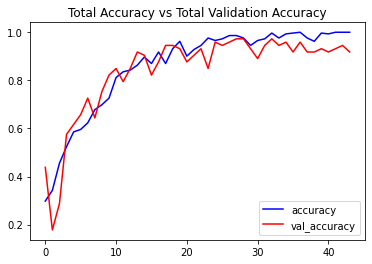
\includegraphics[width=0.5\textwidth]{Figures/acc_model1.png} &
		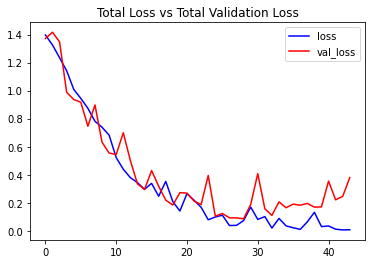
\includegraphics[width=0.5\textwidth]{Figures/loss_model1.png} 
	\end{tabular}
	\caption[Model Accuracy và Model Loss.]{Model Accuracy và Model Loss.}
	\label{fig:modelloss_and_Model Accuracy}
\end{figure}

Đồ thị ACC,  độ chính xác (Accuracy) lên đến 98\% và bắt đầu ổn định khi epoch = 20,  cho cả tập dữ liệu huấn luyện và tập test, đồ thị Loss của cũng cho thấy sau mức này, Loss của cả tập train và validation. Kết quả cho thấy mô hình có độ phù hợp tốt và không bị quá khớp (over-fitting).

\begin{itemize}
	\item Đánh giá hiệu suất mô hình:
	
	\begin{figure}[h!]
		\centering
		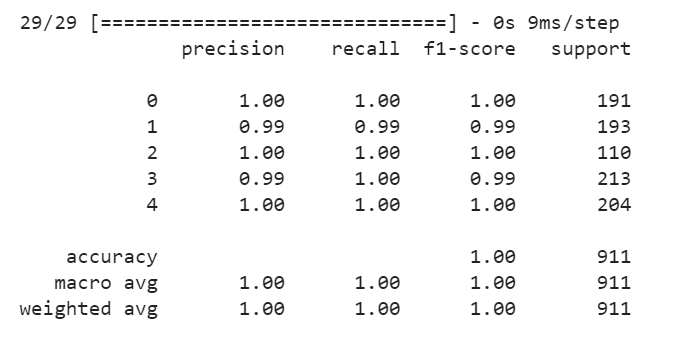
\includegraphics[width=0.7\textwidth]{Figures/evaluate_model1.PNG}
		\caption[Đánh giá hiệu suất mô hình.]{Đánh giá hiệu suất mô hình.}
		\label{fig:ac} 
	\end{figure}
	
	\item Confusion Matrix:
	
	\begin{figure}[h!]
		\centering
		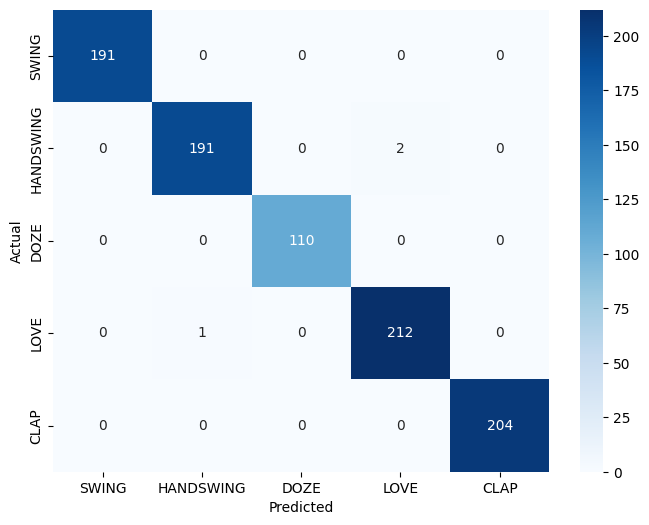
\includegraphics[width=0.6\textwidth]{Figures/model1_confusion.png}
		\caption[Confusion Matrix.]{Confusion Matrix.}
		\label{fig:fu} 
	\end{figure}
\end{itemize}

\subsection{Thử nghiệm với thời gian thực webcam}

*** Sử dụng thư viện open cv để test kết quả trên thời gian thực 

** Bước 1: Import thư viện và Load Model

\begin{lstlisting}[style=codePython]
import cv2
import mediapipe as mp
import numpy as np
import threading
import tensorflow as tf

label = "Warmup...."
n_time_steps = 10
lm_list = []

mpPose = mp.solutions.pose
pose = mpPose.Pose()
mpDraw = mp.solutions.drawing_utils

model = tf.keras.models.load_model("model_19.h5")					
\end{lstlisting}

** Bước 2: Các hàm phụ trợ vẽ điểm nút nối các điểm nút và hàm dự đoán kết quả

\begin{lstlisting}[style=codePython]
def make_landmark_timestep(results):
    c_lm = []
    for id, lm in enumerate(results.pose_landmarks.landmark):
        c_lm.append(lm.x)
        c_lm.append(lm.y)
        c_lm.append(lm.z)
        c_lm.append(lm.visibility)
    return c_lm


def draw_landmark_on_image(mpDraw, results, img):
    mpDraw.draw_landmarks(img, results.pose_landmarks, mpPose.POSE_CONNECTIONS)
    for id, lm in enumerate(results.pose_landmarks.landmark):
        h, w, c = img.shape
        # print(id, lm)
        cx, cy = int(lm.x * w), int(lm.y * h)
        cv2.circle(img, (cx, cy), 5, (255, 0, 0), cv2.FILLED)
    return img


def draw_class_on_image(label, img):
    font = cv2.FONT_HERSHEY_SIMPLEX
    bottomLeftCornerOfText = (10, 30)
    fontScale = 1
    fontColor = (0, 255, 0)
    thickness = 2
    lineType = 2
    cv2.putText(img, label,
                bottomLeftCornerOfText,
                font,
                fontScale,
                fontColor,
                thickness,
                lineType)
    return img


def detect(model, lm_list):
    global label
    lm_list = np.array(lm_list)
    lm_list = np.expand_dims(lm_list, axis=0)
    print(lm_list.shape)

    y_hat = model.predict(lm_list)
    results = np.argmax(y_hat)
    print(y_hat , results)


    label_predict = ('body','hand','doze','love','clap')
    label = label_predict[results]
    return label
\end{lstlisting}

** Bước 3: Chạy webcam

\begin{lstlisting}[style=codePython]
while True:

    success, img = cap.read()
    imgRGB = cv2.cvtColor(img, cv2.COLOR_BGR2RGB)
    results = pose.process(imgRGB)
    i = i + 1
    if i > warmup_frames:
        print("Start detect....")

        if results.pose_landmarks:
            c_lm = make_landmark_timestep(results)

            lm_list.append(c_lm)
            if len(lm_list) == n_time_steps:
                # predict
                t1 = threading.Thread(target=detect, args=(model, lm_list))
                t1.start()
                #t1 = detect(model,lm_list)
                lm_list = []


            img = draw_landmark_on_image(mpDraw, results, img)

    img = draw_class_on_image(label, img)
    cv2.imshow("Image", img)
    if cv2.waitKey(1) == ord('q'):
        break

cap.release()
cv2.destroyAllWindows()							
\end{lstlisting}


\newpage

\section{Xây dựng mô hình sử dụng\href{https://keras.io/api/layers/recurrent_layers/conv_lstm2d/}{ConvLSTM2D layer} và mô hình LRCN}
\subsection{Tiền xử lý dữ liệu}


\subsubsection{Thu thập dữ liệu }

    Trong bài này nhóm xử dụng bộ dự liệu \href{https://www.crcv.ucf.edu/data/UCF50.php}{UCF50 - Action Recognition Dataset}
Bộ dữ liệu Nhận diện hành động, bao gồm các video thực tế được lấy từ YouTube, điều này làm cho bộ dữ liệu này khác biệt so với hầu hết các bộ dữ liệu nhận diện hành động khác vì chúng không phải là thực tế và được đóng bởi diễn viên. Bộ dữ liệu chứa :

\begin{itemize}
    \item 50 Danh mục hành động
    \item 133 Số video trung bình mỗi hành động
    \item 26 Số khung hình trung bình mỗi video
\end{itemize}


\begin{figure}[h!]
	\centering
	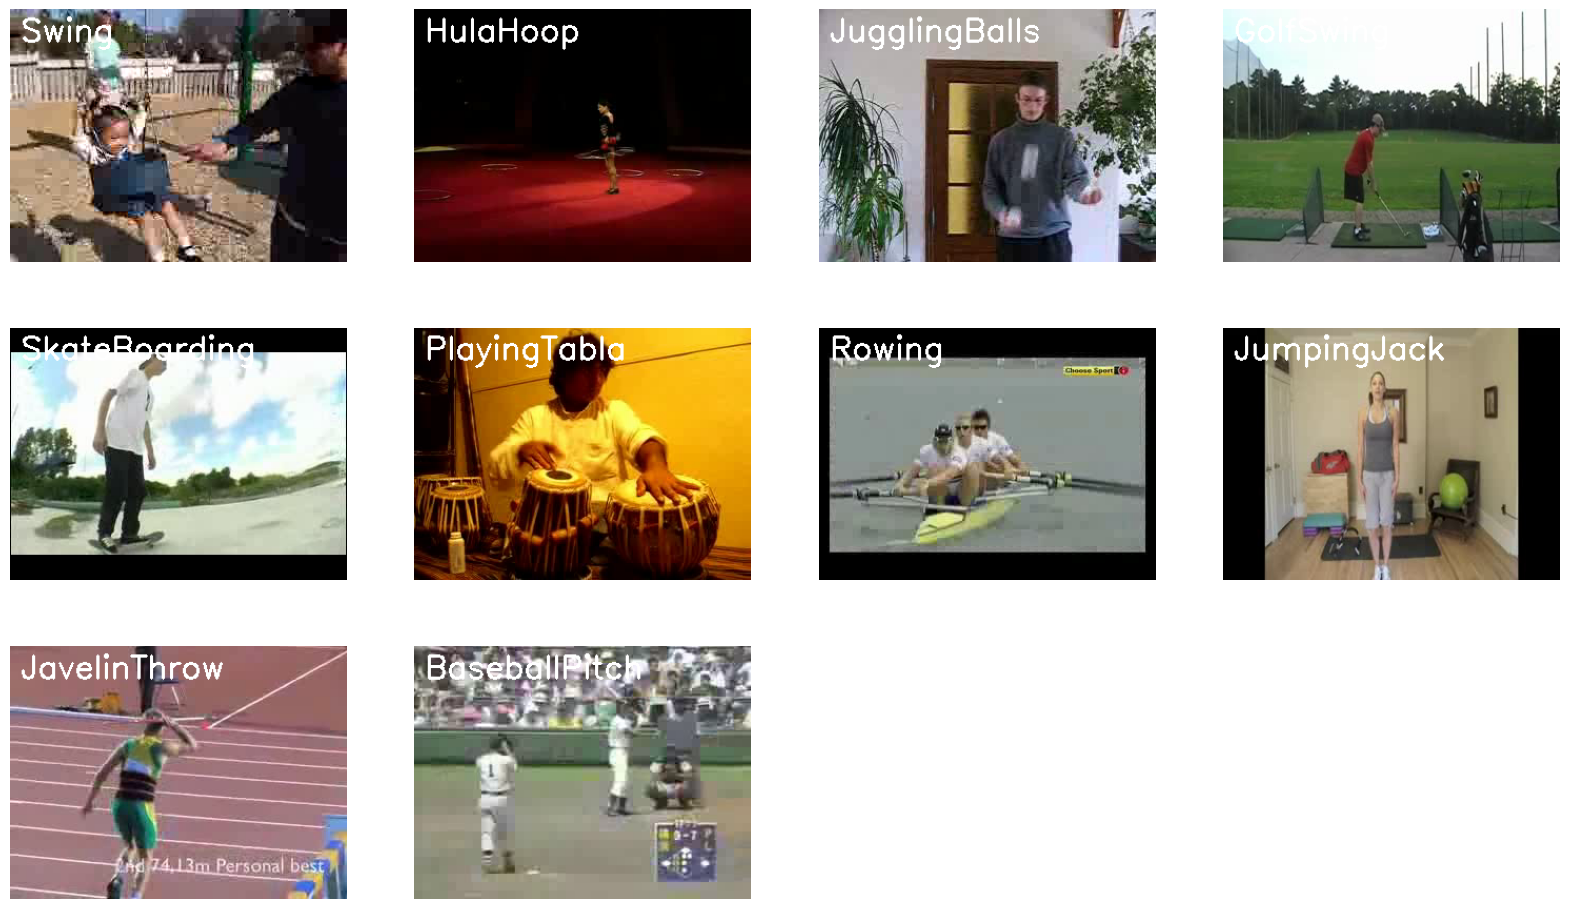
\includegraphics[width=0.7\textwidth]{Figures/datashow.png}
	\caption[Visualize the Data with its Labels.]{Visualize the Data with its Labels .}
	\label{datashow.png} 
    \end{figure}
    \newpage
\subsubsection{Tăng cường dữ liệu}
\begin{figure}[h!]
	\centering
	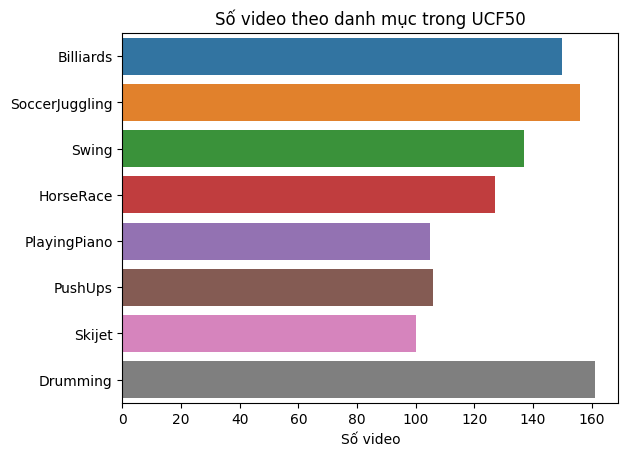
\includegraphics[width=0.7\textwidth]{Figures/numbersvideo.png}
	\caption[Visualize the numbers.]{Visualize the numbers .}
	\label{numbersvideo.png} 
    \end{figure}

Nhận thấy bộ dữ liệu này có sự chênh lệnh về dự liệu cũng như đây là bộ dữ liệu đã có từ 5 năm trước . Hiện nay video đã cải thiện chất lượng hơn . Nhóm đã thêm video tải từ youtube vào để dữ liệu cân bằng cũng như video có độ phân giải tốt hơn để khả năng dự đoán được cải thiện 

Sau khi tăng cường dataset mới được lưu trên drive : \href{https://drive.google.com/drive/folders/1GXIWkXE2PQTgVSl-xattG6JVyaDb1jgR?usp=sharing}{Dataset}
\subsubsection{Chuẩn hóa dữ liệu}
Đầu tiên, chúng ta sẽ đọc các tệp video từ bộ dữ liệu và thay đổi kích thước các khung hình của video thành chiều rộng và chiều cao cố định, để giảm thiểu tính toán và chuẩn hóa dữ liệu về khoảng [0-1] bằng cách chia giá trị pixel cho 255, điều này làm cho quá trình hội tụ nhanh hơn khi huấn luyện mạng.

Nhưng trước hết, hãy khởi tạo một số hằng số.


\begin{lstlisting}[style=codePython]
IMAGE_HEIGHT , IMAGE_WIDTH = 64, 64

SEQUENCE_LENGTH = 10

DATASET_DIR = "UCF50"
\end{lstlisting}

 Tiếp theo tạo một hàm frames\_extraction() sẽ tạo một danh sách chứa các khung hình đã thay đổi kích thước và chuẩn hóa của một video, đường dẫn của video sẽ được truyền vào hàm như một đối số. Hàm sẽ đọc tệp video từng khung hình một, mặc dù không phải tất cả các khung hình được thêm vào danh sách vì chúng ta chỉ cần một chuỗi độ dài khung hình phân phối đều. 

\begin{lstlisting}[style=codePython]
def frames_extraction(video_path):

    frames_list = []
    video_reader = cv2.VideoCapture(video_path)
    video_frames_count =int(video_reader.get(cv2.CAP_PROP_FRAME_COUNT))
    skip_frames_window = max(int(video_frames_count/SEQUENCE_LENGTH), 1)

    for frame_counter in range(SEQUENCE_LENGTH):

        video_reader.set(cv2.CAP_PROP_POS_FRAMES, frame_counter * skip_frames_window)
        
        success, frame = video_reader.read()
        if not success:
            break

        resized_frame = cv2.resize(frame, (IMAGE_HEIGHT, IMAGE_WIDTH))
        normalized_frame = resized_frame / 255
        frames_list.append(normalized_frame)
    video_reader.release()

    return frames_list
\end{lstlisting}

Bây giờ chúng ta sẽ tạo một hàm create\_dataset() sẽ lặp qua tất cả các lớp được chỉ định trong hằng số CLASSES\_LIST và sẽ gọi hàm frame\_extraction() trên mọi tệp video của các lớp được chọn và trả về các khung hình (đặc trưng), chỉ mục lớp (nhãn) và đường dẫn tệp video (video\_files\_paths).

\begin{lstlisting}[style=codePython]
def create_dataset():

    features = []
    labels = []
    video_files_paths = []
    for class_index, class_name in enumerate(CLASSES_LIST):

        print(f'Extracting Data of Class: {class_name}')

        files_list = os.listdir(os.path.join(DATASET_DIR, class_name))

        for file_name in files_list:

            video_file_path = os.path.join(DATASET_DIR, class_name, file_name)

            frames = frames_extraction(video_file_path)

            if len(frames) == SEQUENCE_LENGTH:
                features.append(frames)
                labels.append(class_index)
                video_files_paths.append(video_file_path)
    features = np.asarray(features)
    labels = np.array(labels)

    return features, labels, video_files_paths
\end{lstlisting} 

Cuối cùng ta lại làm các bước chia dữ liệu thành train và test , one hot encode giống như đối với mô hình LSTM đầu tiên 
\begin{lstlisting}[style=codePython]
X, y, video_files_paths = create_dataset()

one_hot_encoded_labels = to_categorical(y)

X_train, X_test, y_train, y_test = train_test_split(X, one_hot_encoded_labels,test_size = 0.2, shuffle = True,random_state = 42)
\end{lstlisting}
Sau khi đã chuẩn bị xong dữ liệu , bước tiếp theo là xây dựng model và đưa dữ liệu đã chuẩn bị vào huấn luyện 
\subsection{Xây dựng mô hình sử dụng ConvLSTM2D layer}
    \begin{figure}[h!]
	\centering
	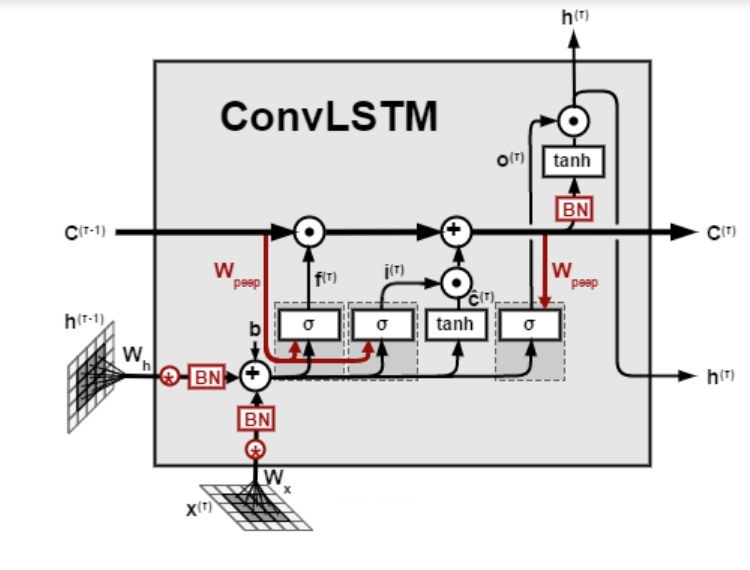
\includegraphics[width=0.7\textwidth]{Figures/convLSTM2D.jpg}
	\caption[ConvLSTM2D layer .]{ConvLSTM2D layer.}
	\label{convLSTM2D.jpg} 
    \end{figure}
Trong bước này, nhóm sẽ thực hiện phương pháp thứ 2 bằng cách sử dụng sự kết hợp của các ô ConvLSTM. Một ô ConvLSTM là một biến thể của mạng LSTM chứa các hoạt động tích chập trong mạng. Điều này là một LSTM với tích chập được nhúng trong kiến trúc, làm cho nó có khả năng xác định các đặc trưng không gian của dữ liệu trong khi vẫn giữ quan hệ thời gian.

Đối với phân loại video, phương pháp này hiệu quả trong việc nắm bắt mối quan hệ không gian trong các khung hình cá nhân và mối quan hệ thời gian qua các khung hình khác nhau. Kết quả của cấu trúc tích chập này, ConvLSTM có khả năng nhận đầu vào 3 chiều (chiều rộng, chiều cao, số kênh) trong khi LSTM đơn giản chỉ nhận đầu vào 1 chiều nên LSTM không tương thích để mô hình dữ liệu không gian-thời gian một cách độc lập.
Tương tự như lớp LSTM, nhưng các phép biến đổi đầu vào và các phép biến đổi hồi quy đều là tích chập.Lớp ConvLSTM2D thường được sử dụng để xử lý các chuỗi ảnh (video) 2 chiều .

ConvLSTM khác với LSTM ở chỗ nó kết hợp cả tính chất không gian (qua các bước tích chập) và tính chất thời gian (qua các bước LSTM), cho phép nó xử lý dữ liệu không gian-thời gian một cách hiệu quả. LSTM thông thường không có khả năng này vì nó chỉ xử lý dữ liệu theo một chiều thời gian.

Để hiểu rõ hơn về ConvLSTM2D hãy đọc bài báo \href{https://keras.io/api/layers/recurrent_layers/conv_lstm2d/}{Convolutional LSTM Network: A Machine Learning Approach for Precipitation Nowcasting} để hiểu hơn về kiến trúc này .

Lớp ConvLSTM2D cần 2 tham số chính:
\begin{itemize}
    \item Số bộ lọc (filters):Xác định số lượng bộ lọc để trích xuất các đặc điểm khác nhau từ ảnh .
    \item  Kích thước kernel (kernel size):Xác định kích thước của bộ lọc hình vuông sẽ được di chuyển trên ảnh để trích xuất các đặc điểm .
\end{itemize}

Đầu ra của lớp ConvLSTM2D là một tensor 4 chiều (batch\_size, timesteps, height, width), với :
\begin{itemize}
    \item batch\_size là số lượng mẫu trong mỗi lần tính toán.
    \item timesteps là số khung hình trong chuỗi ảnh.
    \item height và width là chiều cao và rộng của khung hình.
\end{itemize}


\subsubsection{Kiến trúc mô hình}
\begin{lstlisting}[style=codePython]
    model = Sequential()


    model.add(ConvLSTM2D(filters = 32, kernel_size = (3, 3), activation = 'tanh',data_format = "channels_last",
                         recurrent_dropout=0.2, return_sequences=True, input_shape = (SEQUENCE_LENGTH,IMAGE_HEIGH,IMAGE_WIDTH,3)))

    model.add(MaxPooling3D(pool_size=(1, 2, 2), padding='same', data_format='channels_last'))
    model.add(TimeDistributed(Dropout(0.2)))

    model.add(ConvLSTM2D(filters = 64, kernel_size = (3, 3), activation = 'tanh', data_format = "channels_last",
                         recurrent_dropout=0.2, return_sequences=True))

    model.add(MaxPooling3D(pool_size=(1, 2, 2), padding='same', data_format='channels_last'))
    model.add(TimeDistributed(Dropout(0.2)))

    model.add(ConvLSTM2D(filters = 64, kernel_size = (3, 3), activation = 'tanh', data_format = "channels_last",
                         recurrent_dropout=0.2, return_sequences=True))

    model.add(MaxPooling3D(pool_size=(1, 2, 2), padding='same', data_format='channels_last'))
    model.add(TimeDistributed(Dropout(0.2)))

    model.add(ConvLSTM2D(filters = 128, kernel_size = (3, 3), activation = 'tanh', data_format = "channels_last",
                         recurrent_dropout=0.2, return_sequences=True))

    model.add(MaxPooling3D(pool_size=(1, 2, 2), padding='same', data_format='channels_last'))

    model.add(Flatten())

    model.add(Dense(len(CLASSES_LIST), activation = "softmax"))

    model.summary()

\end{lstlisting}
Các tham số của convLSTM2D có thể hiểu như sau : 
\begin{itemize}
    \item input\_shape = (SEQUENCE\_LENGTH, IMAGE\_HEIGHT, IMAGE\_WIDTH, 3): Kích thước đầu vào, trong đó SEQUENCE\_LENGTH là độ dài chuỗi, IMAGE\_HEIGHT và IMAGE\_WIDTH là kích thước ảnh, và 3 là số kênh màu (RGB).
    \item filters = 32: Số lượng filter hoặc feature maps được áp dụng.
    \item kernel\_size = (3, 3): Kích thước của filter.
    \item activation = 'tanh': Hàm kích hoạt là tanh.
    \item data\_format = "channels\_last": Định dạng dữ liệu là "channels\_last" (chiều cuối cùng là kênh dữ liệu).
    \item recurrent\_dropout = 0.2: Tỷ lệ dropout cho các kết nối tái lặp trong LSTM.
    \item return\_sequences = True: Trả về chuỗi output thay vì chỉ output cuối cùng.
\end{itemize}
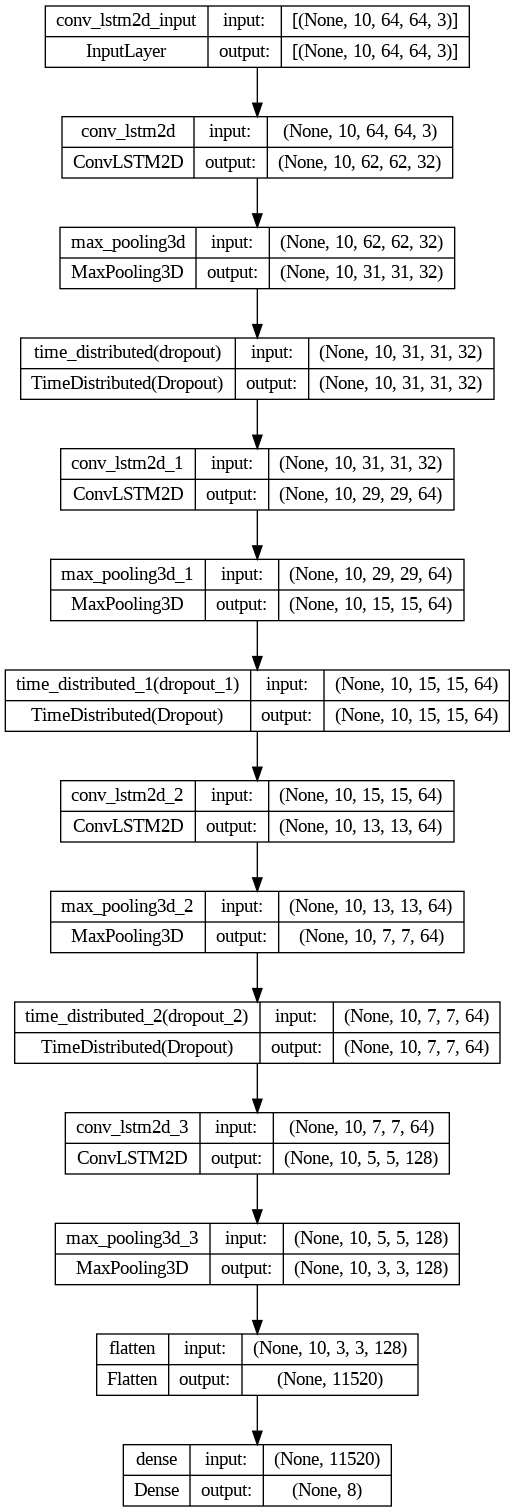
\includegraphics[width=0.5\textwidth]{Figures/model_conv.png}
\begin{figure}[ht!]
	\centering
	
	\caption[Model ConvLSTM2D.]{Model ConvLSTM2D.}
	\label{model_conv.png} 
    \end{figure}


Mô hình nhóm xây dựng để phân biệt 8 hành động , nên nhóm đã để Cuối cùng là 1 lớp kết nối đầy đủ với hàm kích hoạt softmax 
\subsection{Huấn luyện mô hình}
Bước tiếp theo nhóm thực hiện là thiết lập và huấn luyện mô hình 
\begin{lstlisting}[style=codePython]
early_stopping_callback = EarlyStopping(monitor = 'val_loss', patience = 10, mode = 'min', restore_best_weights = True)
convlstm_model.compile(loss = 'categorical_crossentropy', optimizer = 'Adam', metrics = ["accuracy"])

convlstm_model_training_history = convlstm_model.fit(x = X_train, y = y_train, epochs = 40,             
                                  batch_size=32,shuffle = True, validation_split = 0.2,callbacks,[early_stopping_callback])
\end{lstlisting}

Giải thích chi tiết : 
\begin{itemize}
    \item Early Stopping Callback:Sử dụng EarlyStopping callback để theo dõi 'val\_loss', chờ đợi 10 epochs trước khi dừng, theo chế độ 'min' (tối thiểu), và khôi phục trọng số tốt nhất khi kết thúc.
    \item Compile Model:Compile mô hình sử dụng hàm loss là 'categorical\_crossentropy', trình tối ưu hóa là 'Adam', và đánh giá theo chỉ số 'accuracy'.
    \item Training Model:Huấn luyện mô hình sử dụng dữ liệu đầu vào X\_train và nhãn y\_train, với 40 epochs, batch size là 32, xáo trộn dữ liệu, phân chia validation set là 20\%, và sử dụng callbacks bao gồm early\_stopping\_callback.
\end{itemize}

\subsubsection{Đánh giá mô hình}
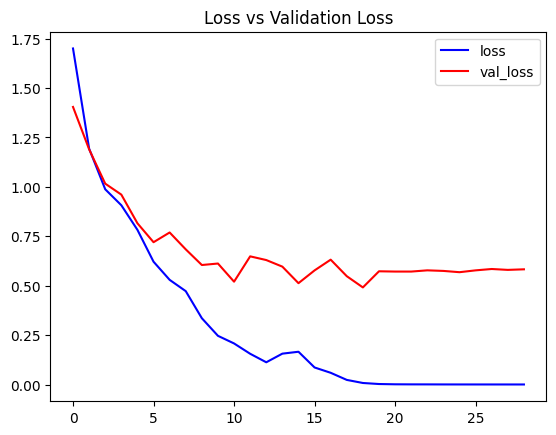
\includegraphics[width=0.5\textwidth]{Figures/loss_conv.png} \&
		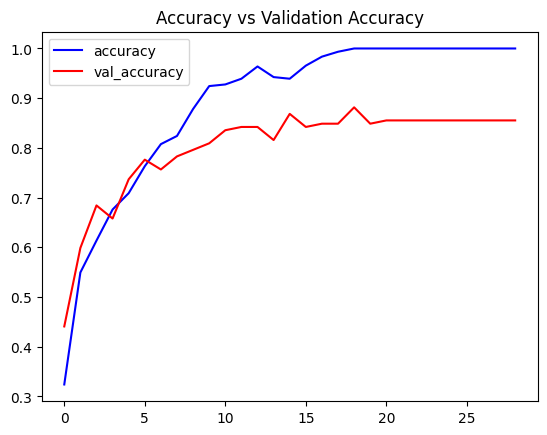
\includegraphics[width=0.5\textwidth]{Figures/val_conv.png}
\begin{figure}[h!] 
	\begin{tabular}{cc}
		\centering
		 
	\end{tabular}
	\caption[Model Accuracy và Model Loss.]{Model Accuracy và Model Loss.}
	\label{fig:modelloss_and_Model Accuracy}
\end{figure}

Đồ thị ACC,  độ chính xác (Accuracy) lên đến 98\% và bắt đầu ổn định khi epoch = 30,  cho cả tập dữ liệu huấn luyện và 86\% tập test, đồ thị Loss của cũng cho thấy sau mức này, Loss của cả tập train và validation. Kết quả cho thấy mô hình có độ phù hợp tốt và không bị quá khớp (over-fitting).

\begin{itemize}
    \item Đánh giá hiệu suất mô hình:
    	
    	\begin{figure}[h!]
    		\centering
    		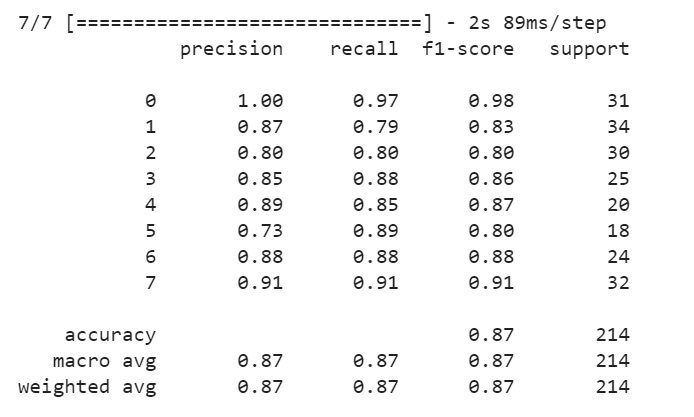
\includegraphics[width=0.7\textwidth]{Figures/evaluate_conv.PNG}
    		\caption[Đánh giá hiệu suất mô hình.]{Đánh giá hiệu suất mô hình.}
    		\label{fig:ac} 
    	\end{figure}
	
	\item Confusion Matrix:
	
	\begin{figure}[h!]
		\centering
		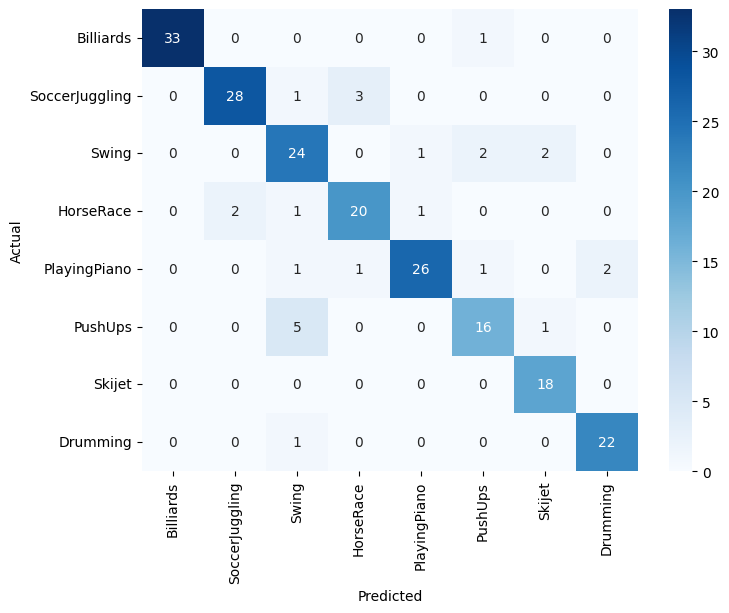
\includegraphics[width=0.6\textwidth]{Figures/conv_confusion.png}
		\caption[Confusion Matrix.]{Confusion Matrix.}
		\label{fig:conv_confusion.png} 
	\end{figure}
\end{itemize}

\subsection{Xây dựng mô hình \href{https://arxiv.org/abs/1411.4389?source=post_page---------------------------}{LRCN}}
    \begin{figure}[h!]
	\centering
	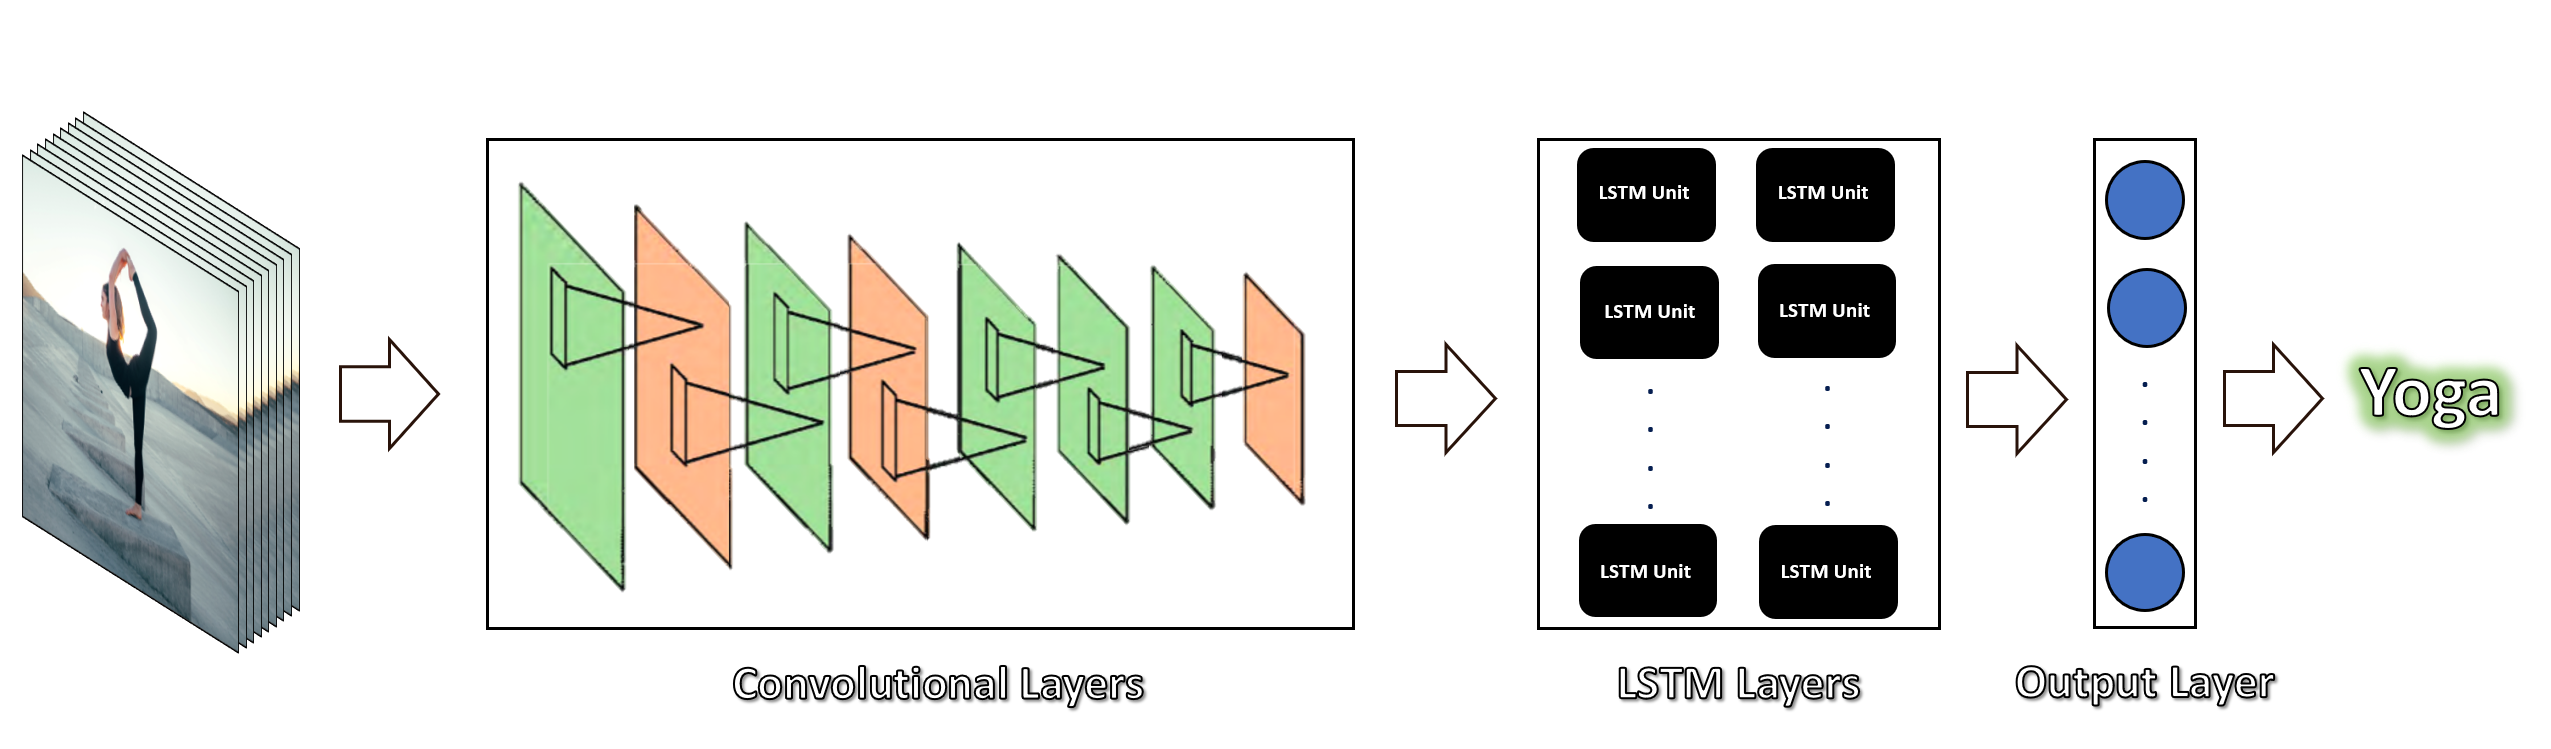
\includegraphics[width=0.7\textwidth]{Figures/LRCN.png}
	\caption[LRCN model .]{LRCN model.}
	\label{LRCN.png} 
    \end{figure}
Trong bước này, nhóm sẽ thực hiện phương pháp thứ 3 xây dựng mô hình LRCN ( Long-Term Recurrent Convolutional Network)

Mô hình LRCN (Long-Term Recurrent Convolutional Network) là một mô hình học sâu được sử dụng cho các tác vụ xử lý dữ liệu hình ảnh tuần tự, chẳng hạn như phân loại video, nhận dạng hành động và chú thích hình ảnh.

Mô hình LRCN là một mô hình kết hợp các lớp Convolutional và LSTM trong một mô hình duy nhất.Mô hình LRCN bao gồm hai thành phần chính:
\begin{itemize}
    \item Các lớp Convolutional trích xuất các đặc trưng không gian từ từng khung hình.
    \item Các đặc trưng này được đưa trực tiếp vào các lớp LSTM tại từng bước thời gian để mô hình chuỗi thời gian.
\end{itemize}
Cách tiếp cận này cho phép mô hình học trực tiếp các đặc trưng không gian thời gian trong quá trình huấn luyện end-to-end, dẫn đến một mô hình mạnh mẽ hơn.
Cụ thể, mô hình LRCN hoạt động như sau:
\begin{itemize}
    \item Dữ liệu đầu vào (các sequence hình ảnh) được đưa vào các lớp convolution 2D. Các lớp convolution 2D sẽ trích xuất các đặc trưng không gian từ từng frame trong sequence.
    \item Các đặc trưng không gian từ các frames được kết hợp lại và đưa vào lớp LSTM. Lớp LSTM sẽ xử lý thông tin thời gian giữa các frames.
    \item Lớp LSTM sẽ tạo ra một vector biểu diễn cho toàn bộ sequence.
    \item Vector biểu diễn này được đưa vào một lớp phân loại để dự đoán kết quả của tác vụ.
\end{itemize}

Mô hình LRCN có một số ưu điểm sau:
\begin{itemize}
    \item Có thể trích xuất các đặc trưng không gian và thời gian từ dữ liệu hình ảnh tuần tự.
    \item Có thể nắm bắt các mối quan hệ dài hạn giữa các frames trong một sequence.
    \item Có thể huấn luyện end-to-end, đơn giản hóa quá trình huấn luyện.
\end{itemize}

Tuy nhiên, mô hình LRCN cũng có một số nhược điểm sau:
\begin{itemize}
    \item Có thể gặp khó khăn trong việc nắm bắt các mối quan hệ phức tạp giữa các đặc trưng không gian và thời gian.
    \item Có thể khó huấn luyện.

\end{itemize}

Mô hình LRCN đã được áp dụng thành công cho nhiều tác vụ xử lý dữ liệu hình ảnh tuần tự, chẳng hạn như:
\begin{itemize}
    \item Phân loại video
    \item Nhận dạng hành động
    \item Chú thích hình ảnh
    \item Theo dõi đối tượng
\end{itemize}

Dưới đây là một số ví dụ về ứng dụng của mô hình LRCN:
\begin{itemize}
    \item Phân loại video thành các loại khác nhau, chẳng hạn như thể thao, tin tức, giải trí, v.v.
    \item Nhận dạng các hành động của con người trong video, chẳng hạn như đi bộ, chạy, nhảy, v.v.
    \item Chú thích hình ảnh bằng văn bản, chẳng hạn như mô tả nội dung của hình ảnh.
    \item Theo dõi đối tượng trong video, chẳng hạn như xác định vị trí của một người trong video.
\end{itemize}



\subsubsection{Kiến trúc mô hình}
\begin{lstlisting}[style=codePython]
def create_LRCN_model():


    model = Sequential()


    model.add(TimeDistributed(Conv2D(16, (3, 3), padding='same',activation = 'relu'),
                              input_shape = (SEQUENCE_LENGTH, IMAGE_HEIGHT, IMAGE_WIDTH, 3)))

    model.add(TimeDistributed(MaxPooling2D((4, 4))))
    model.add(TimeDistributed(Dropout(0.25)))

    model.add(TimeDistributed(Conv2D(32, (3, 3), padding='same',activation = 'relu')))
    model.add(TimeDistributed(MaxPooling2D((4, 4))))
    model.add(TimeDistributed(Dropout(0.25)))

    model.add(TimeDistributed(Conv2D(64, (3, 3), padding='same',activation = 'relu')))
    model.add(TimeDistributed(MaxPooling2D((2, 2))))
    model.add(TimeDistributed(Dropout(0.25)))

    model.add(TimeDistributed(Conv2D(64, (3, 3), padding='same',activation = 'relu')))
    model.add(TimeDistributed(MaxPooling2D((2, 2))))
    #model.add(TimeDistributed(Dropout(0.25)))

    model.add(TimeDistributed(Flatten()))

    model.add(LSTM(32))

    model.add(Dense(len(CLASSES_LIST), activation = 'softmax'))


    model.summary()


    return model

\end{lstlisting}
Lớp TimeDistributed(Conv2D) thực hiện các bước sau : 
\begin{itemize}
    \item TimeDistributed: Đảm bảo lớp Conv2D được áp dụng cho từng frame riêng lẻ trong chuỗi hình ảnh.
    \item Conv2D(16, (3, 3), padding='same', activation='relu'): Tạo một lớp convolutional 2D với các thông số sau:
    \item input\_shape = (SEQUENCE\_LENGTH, IMAGE\_HEIGHT, IMAGE\_WIDTH, 3): Kích thước đầu vào, trong đó SEQUENCE\_LENGTH là độ dài chuỗi, IMAGE\_HEIGHT và IMAGE\_WIDTH là kích thước ảnh, và 3 là số kênh màu (RGB).
\end{itemize}
\newpage
\begin{figure}[h!]
	\centering
	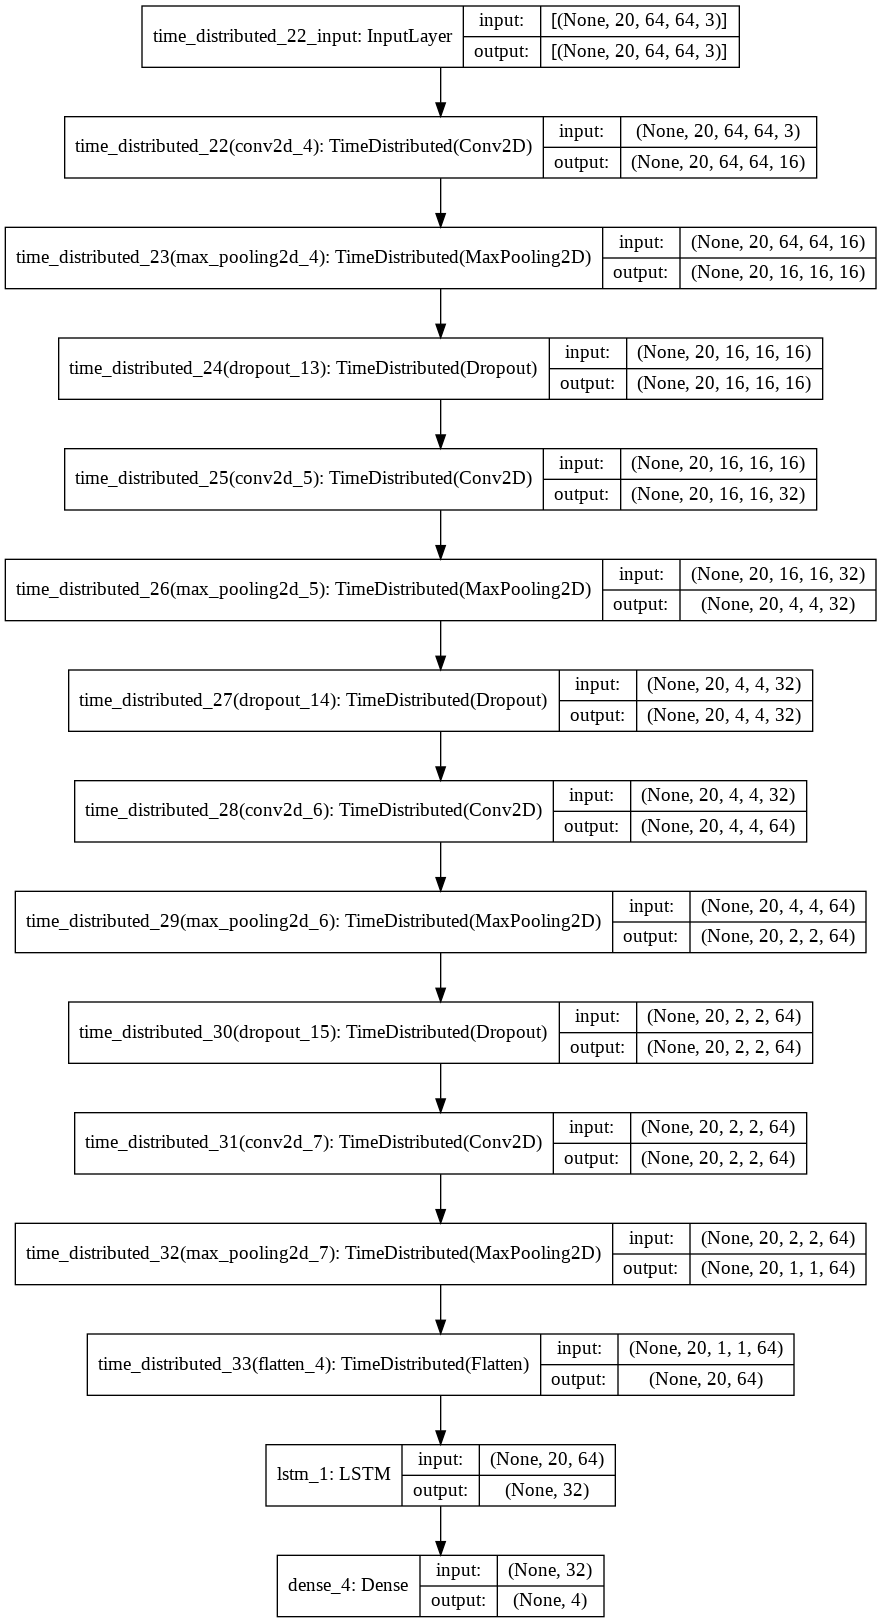
\includegraphics[width=0.7\textwidth]{Figures/model_lrcn.png}
	\caption[Kiến trúc model LRCN.]{Kiến trúc model LRCN.}
	\label{model_lrcn.png} 
    \end{figure}
\newpage
Mô hình nhóm xây dựng để phân biệt 8 hành động , nên nhóm đã để Cuối cùng là 1 lớp kết nối đầy đủ với hàm kích hoạt softmax 

Bước tiếp theo nhóm thực hiện là thiết lập và huấn luyện mô hình  áp dụng giống như cách làm với mô hình sử dụng convLSTM2D

\subsubsection{Đánh giá mô hình}
		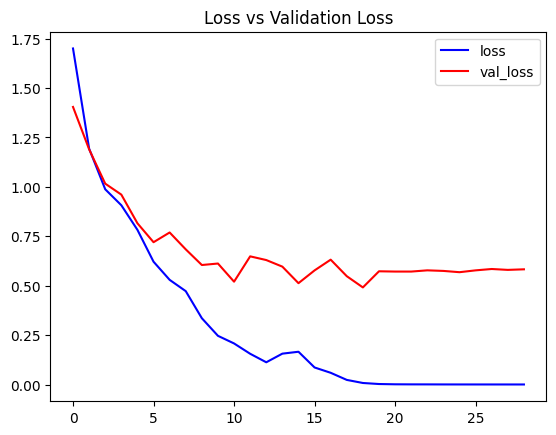
\includegraphics[width=0.5\textwidth]{Figures/loss_conv.png} \&
		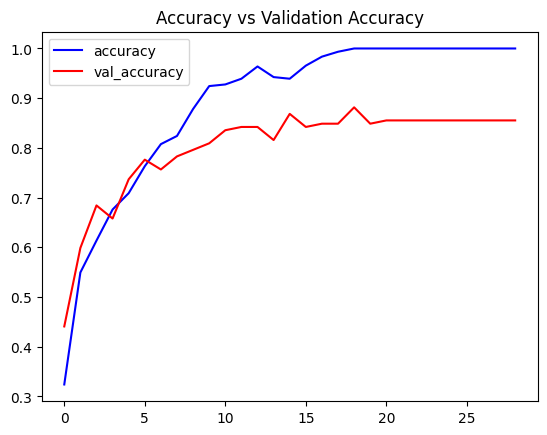
\includegraphics[width=0.5\textwidth]{Figures/val_conv.png}
\begin{figure}[h!] 
	\begin{tabular}{cc}
		\centering
    
	\end{tabular}
	\caption[Model Accuracy và Model Loss.]{Model Accuracy và Model Loss.}
	\label{fig:modelloss_and_Model Accuracy}
\end{figure}

Đồ thị ACC,  độ chính xác (Accuracy) lên đến 97\% và bắt đầu ổn định khi epoch = 20,  cho cả tập dữ liệu huấn luyện và và 90\% tập test, đồ thị Loss của cũng cho thấy sau mức này, Loss của cả tập train và validation. Kết quả cho thấy mô hình có độ phù hợp tốt và không bị quá khớp (over-fitting).
\newpage
\begin{itemize}
	\item Đánh giá hiệu suất mô hình:
 
	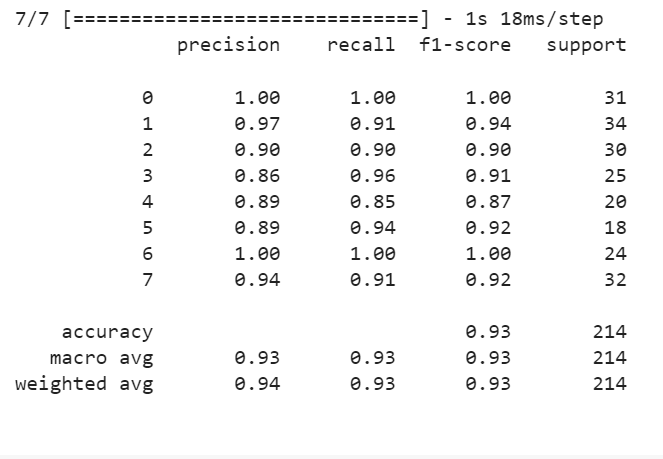
\includegraphics[width=0.7\textwidth]{Figures/evaluate_lrcn.PNG}
	\begin{figure}[h!] 
	\begin{tabular}{cc}
		\centering
	\end{tabular}
	\caption[Đánh giá hiệu suất mô hình.]{Đánh giá hiệu suất mô hình.}
	\label{fig:modelloss_and_Model Accuracy}
\end{figure}
	\item Confusion Matrix:
	
	\begin{figure}[h!]
		\centering
		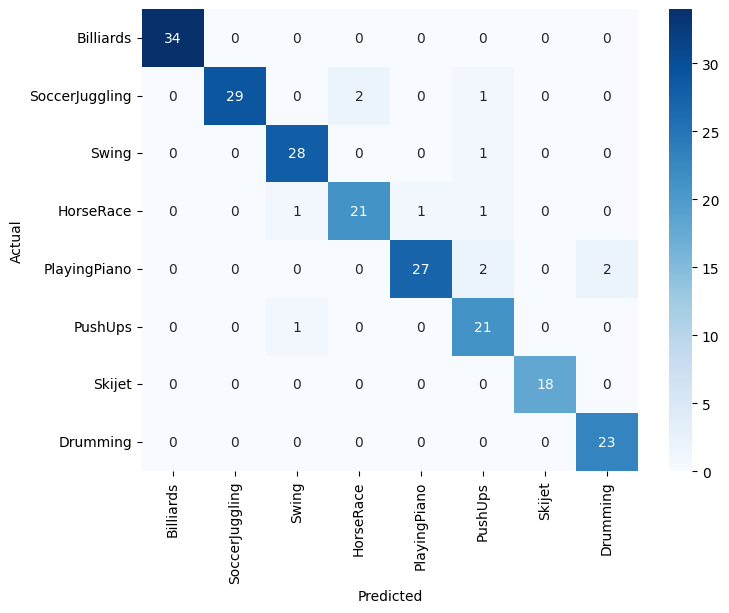
\includegraphics[width=0.6\textwidth]{Figures/lstm_confusion.png}
		\caption[Confusion Matrix.]{Confusion Matrix.}
		\label{fig:lstm_confusion} 
	\end{figure}
\end{itemize}
\subsection{Thử nghiệm với video download từ youtube}
Bước 1 : Download video từ youtube : 
Hàm download\_youtube\_video có nhiệm vụ download video từ link youtube .
\begin{lstlisting}[style=codePython]
def download_youtube_video(url, output_path):
    try:
        youtube = pytube.YouTube(url)
        video = youtube.streams.get_highest_resolution()
        title = video.title
        output_file_path = f"{output_path}/{title}.mp4"
        video.download(output_path)
        return title
    except Exception as e:
        print("Error: ", str(e))
        return None
\end{lstlisting}

Bước 2 : Viết hàm dự đoán hành động trong video 

\begin{lstlisting}[style=codePython]
def predict_on_video(video_file_path, output_file_path, SEQUENCE_LENGTH):


    video_reader = cv2.VideoCapture(video_file_path)

    original_video_width = int(video_reader.get(cv2.CAP_PROP_FRAME_WIDTH))
    original_video_height = int(video_reader.get(cv2.CAP_PROP_FRAME_HEIGHT))

    video_writer = cv2.VideoWriter(output_file_path, cv2.VideoWriter_fourcc('M', 'P', '4', 'V'),
                                   video_reader.get(cv2.CAP_PROP_FPS), (original_video_width, original_video_height))

    frames_queue = deque(maxlen = SEQUENCE_LENGTH)

    predicted_class_name = ''

    while video_reader.isOpened():

        _, frame = video_reader.read()

        if not _:
            break

        resized_frame = cv2.resize(frame, (IMAGE_HEIGHT, IMAGE_WIDTH))

        normalized_frame = resized_frame / 255

        frames_queue.append(normalized_frame)

        if len(frames_queue) == SEQUENCE_LENGTH:

            predicted_labels_probabilities = convlstm_model.predict(np.expand_dims(frames_queue, axis = 0))[0]

            predicted_label = np.argmax(predicted_labels_probabilities)

            predicted_class_name = CLASSES_LIST[predicted_label]

        cv2.putText(frame, predicted_class_name, (10, 30), cv2.FONT_HERSHEY_SIMPLEX, 1, (0, 255, 0), 2)

        video_writer.write(frame)

    video_reader.release()
    video_writer.release()
\end{lstlisting}


Trong đoạn code trên cần chú ý  : 
\begin{itemize}
    \item frames\_queue = deque(maxlen=SEQUENCE\_LENGTH): Tạo một hàng đợi (queue) để lưu trữ các khung hình, giới hạn số lượng khung hình tối đa là SEQUENCE\_LENGTH. 
\end{itemize}

% Chương 4 

\chapter{DEMO VÀ ĐÁNH GIÁ PHƯƠNG PHÁP} 

\label{Chapter4}

\section{Demo sản phẩm}



\subsection{Sử dụng công cụ MediaPipe và xây dựng mạng LSTM}
\begin{itemize}
    \item Swing
    
        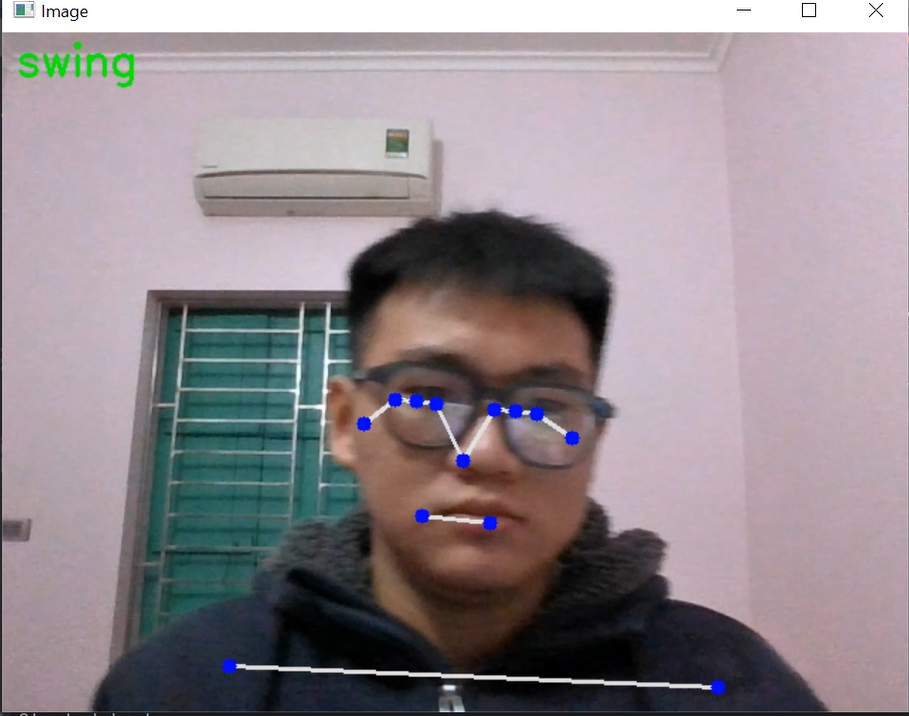
\includegraphics[width=0.5\textwidth]{Figures/swing.PNG}
        \begin{figure}[h!]
    	\centering
    	\caption[Swing output .]{Swing output.}
    	\label{bia_conv.png} 
        \end{figure}
    \item Hand Swing

        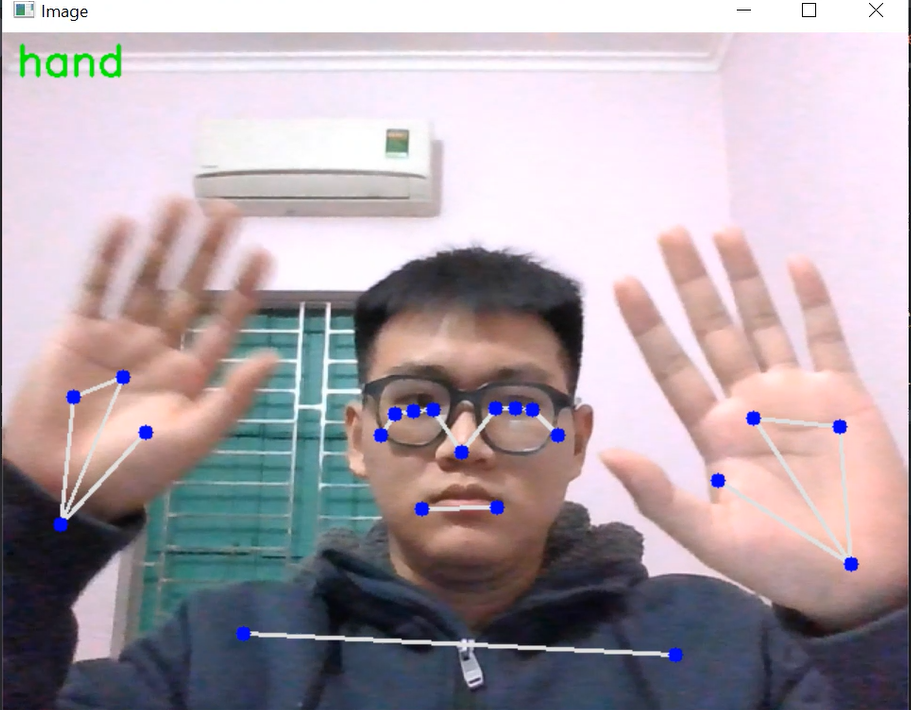
\includegraphics[width=0.5\textwidth]{Figures/hand.PNG}
        \begin{figure}[h!]
    	\centering
    	
    	\caption[Hand Swing output .]{Hand Swing output.}
    	\label{hand.png} 
        \end{figure}
    \item Love

        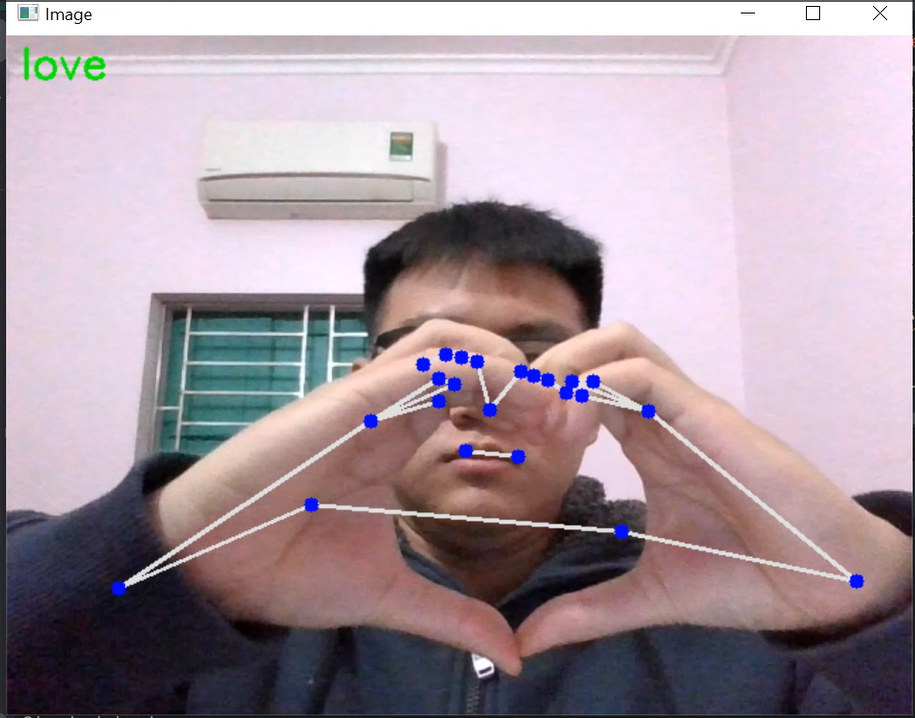
\includegraphics[width=0.5\textwidth]{Figures/love.PNG}
        \begin{figure}[h!]
    	\centering
    	
    	\caption[Love output .]{Love output.}
    	\label{love.png} 
        \end{figure}
        
    \item Clap

        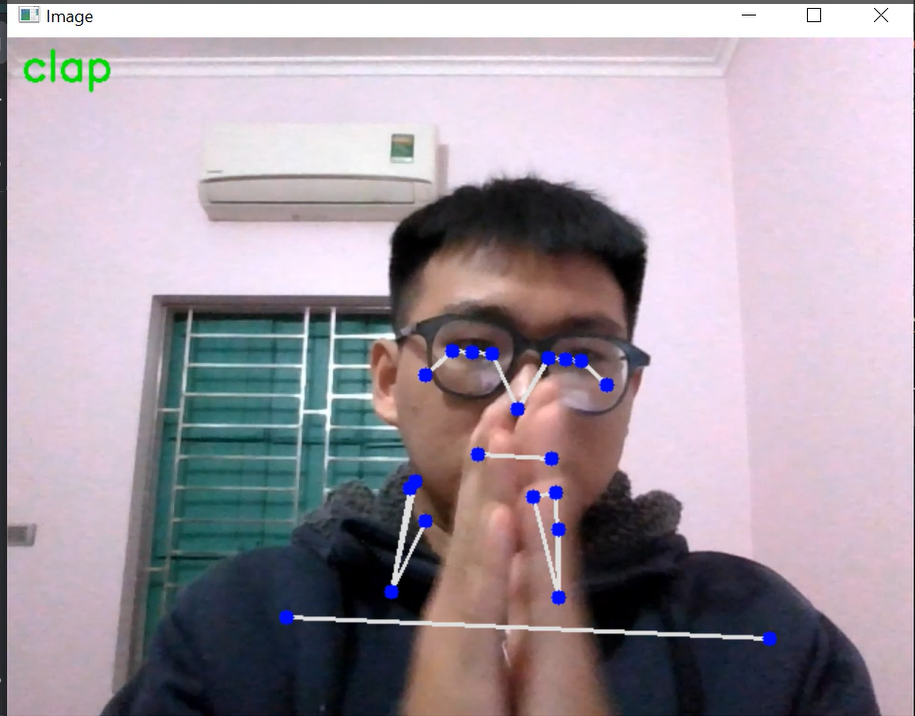
\includegraphics[width=0.5\textwidth]{Figures/clap.PNG}
        \begin{figure}[h!]
    	\centering
    	
    	\caption[Clap output .]{Clap output.}
    	\label{clap.png} 
        \end{figure}

    \item Doze

        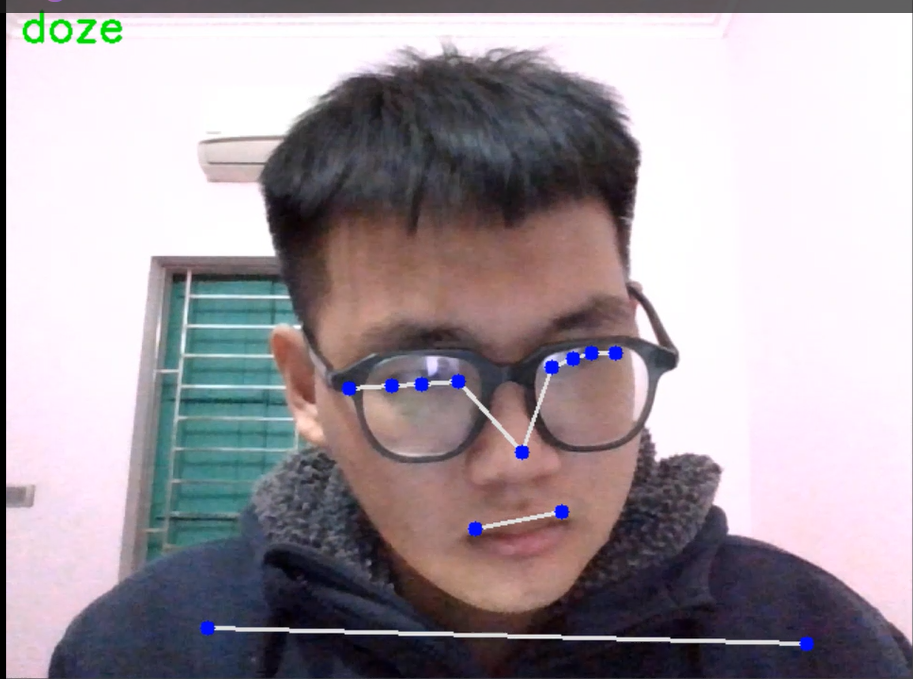
\includegraphics[width=0.5\textwidth]{Figures/doze.PNG}
        \begin{figure}[h!]
    	\centering
    	
    	\caption[Doze output .]{Doze output.}
    	\label{doze.png} 
        \end{figure}
\end{itemize}

\subsection{Mô hình ConvLSTM}
\begin{itemize}
    \item Billards
    
        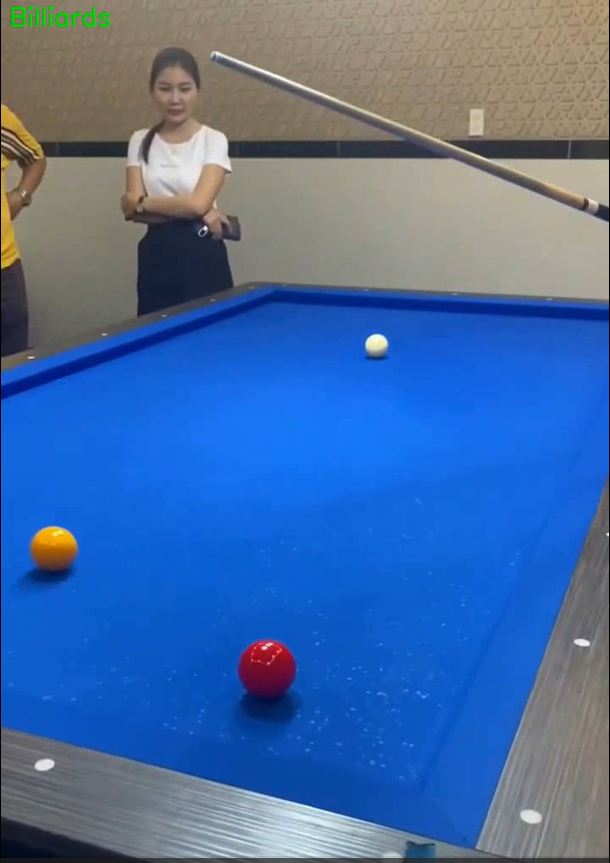
\includegraphics[width=0.5\textwidth]{Figures/bia_conv.png}
        \begin{figure}[h!]
    	\centering
    	\caption[Billards output .]{Billards output.}
    	\label{bia_conv.png} 
        \end{figure}
    \item Soccer Juggling

        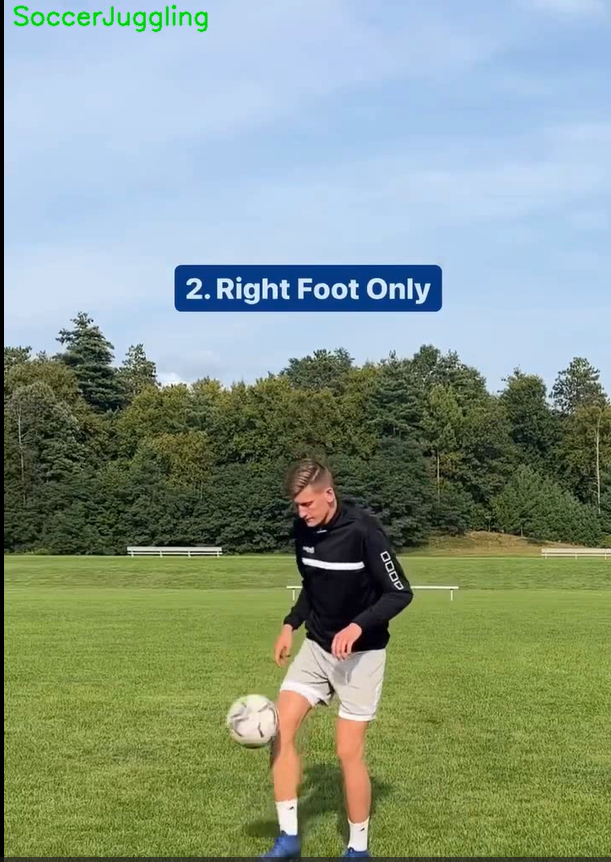
\includegraphics[width=0.5\textwidth]{Figures/soccer_conv.png}
        \begin{figure}[h!]
    	\centering
    	
    	\caption[Soccer Juggling output .]{Soccer Juggling output.}
    	\label{soccer_conv.png} 
        \end{figure}
    \item Swing

        \includegraphics[width=0.5\textwidth]{Figures/swing_conv.png}
        \begin{figure}[h!]
    	\centering
    	
    	\caption[Swing output .]{Swing output.}
    	\label{swing_conv.png} 
        \end{figure}
        
    \item HorseRace

        \includegraphics[width=0.5\textwidth]{Figures/race_conv.png}
        \begin{figure}[h!]
    	\centering
    	
    	\caption[HorseRace output .]{HorseRace output.}
    	\label{race_conv.png} 
        \end{figure}

    \item PlayingPiano

        \includegraphics[width=0.5\textwidth]{Figures/piano_conv.png}
        \begin{figure}[h!]
    	\centering
    	
    	\caption[PlayingPiano output .]{PlayingPiano output.}
    	\label{piano_conv.png} 
        \end{figure}

    \item PushUps

        \includegraphics[width=0.5\textwidth]{Figures/pushup_conv.png}
        \begin{figure}[h!]
    	\centering
    	
    	\caption[PushUps output .]{PushUps output.}
    	\label{pushup_conv.png} 
        \end{figure}
        
    \item Skijet

        \includegraphics[width=0.5\textwidth]{Figures/skijet_conv.png}
        \begin{figure}[h!]
    	\centering
    	
    	\caption[Skijet output .]{Skijet output.}
    	\label{skijet_conv.png} 
        \end{figure}

    \item Drumming

        \includegraphics[width=0.5\textwidth]{Figures/drum_conv.png}
        \begin{figure}[h!]
    	\centering
    	
    	\caption[Drumming output .]{Drumming output.}
    	\label{drum_conv.png} 
        \end{figure}
    
\end{itemize}
    


\subsection{Mô hình LRCN}

\begin{itemize}
    \item Billards
    
        \includegraphics[width=0.5\textwidth]{Figures/bia_lrcn.png}
        \begin{figure}[h!]
    	\centering
    	\caption[Billards output .]{Billards output.}
    	\label{bia_lrcn.png} 
        \end{figure}
    \item Soccer Juggling

        \includegraphics[width=0.5\textwidth]{Figures/soccer_lrcn.png}
        \begin{figure}[h!]
    	\centering
    	
    	\caption[Soccer Juggling output .]{Soccer Juggling output.}
    	\label{soccer_lrcn.png} 
        \end{figure}
    \item Swing

        \includegraphics[width=0.5\textwidth]{Figures/swing_lrcn.png}
        \begin{figure}[h!]
    	\centering
    	
    	\caption[Swing output .]{Swing output.}
    	\label{swing_lrcn.png} 
        \end{figure}
        
    \item HorseRace

        \includegraphics[width=0.5\textwidth]{Figures/race_lrcn.png}
        \begin{figure}[h!]
    	\centering
    	
    	\caption[HorseRace output .]{HorseRace output.}
    	\label{race_lrcn.png} 
        \end{figure}

    \item PlayingPiano

        \includegraphics[width=0.5\textwidth]{Figures/piano_lrcn.png}
        \begin{figure}[h!]
    	\centering
    	
    	\caption[PlayingPiano output .]{PlayingPiano output.}
    	\label{piano_lrcn.png} 
        \end{figure}

    \item PushUps

        \includegraphics[width=0.5\textwidth]{Figures/pushup_lrcn.png}
        \begin{figure}[h!]
    	\centering
    	
    	\caption[PushUps output .]{PushUps output.}
    	\label{pushup_lrcn.png} 
        \end{figure}
        
    \item Skijet

        \includegraphics[width=0.5\textwidth]{Figures/skijet_lrcn.png}
        \begin{figure}[h!]
    	\centering
    	
    	\caption[Skijet output .]{Skijet output.}
    	\label{skijet_lrcn.png} 
        \end{figure}

    \item Drumming

        \includegraphics[width=0.5\textwidth]{Figures/drum_lrcn.png}
        \begin{figure}[h!]
    	\centering
    	
    	\caption[Drumming output .]{Drumming output.}
    	\label{drum_lrcn.png} 
        \end{figure}
    
\end{itemize}



\section{Đánh giá các phương pháp}

Trong dự án này ,nhóm đã tiếp cận bài toán theo 3 phương pháp tùy thuộc vào độ phức tạp , độ chính xác cần thiết và khả năng tính toán.Đối với phương pháp sử dụng thư viện mediapipe kết hợp với LSTM phù hợp với các bài toán đơn giản , nhận diện ít hành động.Đối với nhận diện hành động qua video , Nhóm nhận thấy phương pháp xây dựng model LRCN cho ra kết quả nhận diện hành động từ video tốt hơn phương pháp sử dụng ConvLSTM . Tuy nhiên tùy thuộc vào từng bài toán mà chúng ta chọn phương pháp sao cho hiệu quả nhất . 

\begin{itemize}
    \item Model ConvLSTM sử dụng các lớp ConvLSTM2D để học các đặc trưng tĩnh và động từ các khung hình video cùng một lúc.
    \item Model LRCN sử dụng các lớp TimeDistributed(Conv2D) để trích xuất các đặc trưng tĩnh từ từng khung hình riêng lẻ, sau đó mới đưa các đặc trưng này vào một lớp LSTM để học các mối quan hệ động giữa các khung hình.
\end{itemize}
\subsection{Cách tiếp cận sử dụng ConvLSTM2D}
- Các lớp ConvLSTM2D trích xuất các đặc trưng không gian thời gian đồng thời duy trì mối quan hệ không gian.
- Học các đặc trưng không gian và thời gian đồng thời bằng cách tích hợp các phép toán tích chập trực tiếp vào các lớp LSTM.
- Các phép toán tích chập được sử dụng để trích xuất đặc trưng không gian từ các khung hình, trong khi các cổng LSTM được sử dụng để học các mối quan hệ thời gian giữa các khung hình.
- Độ phức tạp của video: ConvLSTM có thể phù hợp hơn cho các video có các hành động phức tạp hoặc dài.
- Độ chính xác cần thiết: ConvLSTM có thể đạt được độ chính xác cao hơn trong một số trường hợp.
- Khả năng tính toán: ConvLSTM thường đòi hỏi nhiều tài nguyên tính toán hơn so với LRCN.
\subsection{Cách tiếp cận sử dụng LRCN}

- LRCN kết hợp các lớp CNN và LSTM trong cùng một mô hình.
- Các lớp CNN được sử dụng để trích xuất các đặc trưng không gian từ các frames.
- Các đặc trưng không gian được đưa vào các lớp LSTM tại mỗi bước thời gian để mô hình hóa chuỗi thời gian.
- Cách tiếp cận này cho phép mô hình học trực tiếp các đặc trưng không gian thời gian trong quá trình huấn luyện end-to-end, dẫn đến một mô hình mạnh mẽ hơn.
- Trong LRCN, lớp TimeDistributed được sử dụng để áp dụng cùng một lớp cho mọi khung hình của video một cách độc lập.
- Lớp TimeDistributed cho phép model LRCN xử lý toàn bộ video trong một lần, thay vì phải xử lý từng khung hình riêng lẻ.

Ưu điểm của LRCN:
\begin{itemize}
    \item Có thể học các đặc trưng không gian thời gian trực tiếp từ dữ liệu .
    \item Có thể nắm bắt các mối quan hệ dài hạn giữa các frames trong một sequence .
    \item Có thể huấn luyện end-to-end, đơn giản hóa quá trình huấn luyện .
\end{itemize}

Nhược điểm của LRCN:

\begin{itemize}
    \item Có thể khó huấn luyện hơn so với cách tiếp cận sử dụng CNN và LSTM riêng biệt.
    \item Có thể gặp khó khăn trong việc nắm bắt các mối quan hệ phức tạp giữa các đặc trưng không gian và thời gian.
\end{itemize}


Khi nào nên chọn LRCN:
\begin{itemize}
    \item Khi cần nắm bắt các mối quan hệ dài hạn giữa các frames trong một sequence.
    \item Khi cần một mô hình mạnh mẽ có thể học các đặc trưng không gian thời gian trực tiếp từ dữ liệu.
\end{itemize}



\section{Hướng phát triển trong tương lai}

\begin{itemize}
	\item Trong tương lai, nhóm muốn tạo ra một app trên điện thoại để có thể đến được gần hơn với nhiều người. 
	
	\item Muốn phát triển lên thành sản phẩm hoàn chỉnh có tính thực tế cao hơn.	
	
	\item Cải thiện model tốt hơn , dự đoán chính xác hơn , nhanh hơn . 
\end{itemize}



 
\chapter*{KẾT LUẬN}
\addcontentsline{toc}{chapter}{KẾT LUẬN}

\label{Chapter5}

Bài viết này mang đến cho bạn đọc một vài giải pháp trong bài toán nhận diện hành động của con người trong video.

Kết quả thực nghiệm cho thấy mô hình nhận dạng sử dụng các thuật toán phân loại phổ biến và tập đặc trưng của chúng tôi cho kết quả rất tốt với các hoạt động thường ngày của con người. Việc đơn giản hoá bộ đặc trưng và lựa chọn kích thước cửa sổ tối ưu từ việc phân tích đặc điểm dữ liệu có thể làm cải thiện tốc độ nhận dạng mà vẫn đảmbảo độ chính xác. Ngoài ra, việc lựa chọn một thuật toán phân loại thích hợp cũng ảnh hưởng rõ rệt tới kết quả nhận dạng. Đối với mô hình thử nghiệm của chúng tôi, thuật toán CNN giúp cải thiện độ chính xác hơn so với DecisionTree, Gradient Boosted Tree, SVM, RF, KNN. Tuy nhiên,hành vi của con người không chỉ là tự nhiên và tự phát,mà con người có thể thực hiện một số hoạt động cùng mộtlúc, hoặc thậm chí thực hiện một số hoạt động không liên quan. Đây cũng là thách thức lớn trong bài toán nhận dạng hành động với thời gian thực. Trong tương lai, chúng tôi tiếp tục phát triển hệ thống của mình để có thể dự đoán và xác định các hoạt động đồng thời, hỗ trợ ứng dụng cho các hoàn cảnh sử dụng phức tạp hơn, hướng tới các ứng dụng không chỉ gắn với con người 

Có rất nhiều thứ có thể cải tiến để có được kết quả tốt hơn mà bạn có thể thử nếu áp dụng vào bài toán thực tế:
\begin{itemize}
    \item Tăng FPS để có thể chạy được realtime: Tối ưu hóa model (pruning, quantization), loại bỏ bớt frame khi nhận diện, sử dụng multi-threading, ...
    \item Sử dụng các Pose Estimation model khác như AlphaPose, OpenPose, ...
\end{itemize}




 



%----------------------------------------------------------------------------------------
%	(KHÔNG CHỈNH SỬA PHẦN NÀY)
%
%	PHẦN 10: TÀI LIỆU THAM KHẢO
%----------------------------------------------------------------------------------------

\begin{spacing}{1.15}
	\printbibliography[heading=bibintoc, title=Tài liệu tham khảo] % In ra tài liệu tham khảo
\end{spacing}

\cite{Reference1,Reference2,Reference3,Reference4,Reference5,Bisong2019}

%----------------------------------------------------------------------------------------
%	PHẦN 11: PHỤ LỤC (THESIS CONTENT - APPENDICES)
%----------------------------------------------------------------------------------------

%\appendix % Nói với LaTeX rằng những chương về sau được tính là phụ lục

% Hãy thêm những phụ lục (appendix) của khóa luận/tiểu luận vào thư mục Appendices
% Hãy bỏ chú thích những dòng nếu bạn đã bổ sung những phụ lục vào

\chapter*{Code}
\addcontentsline{toc}{chapter}{Code}

\label{Mã nguồn hệ thống}

Toàn hộ source code ,model và video demo output project được chia sẻ tại : \href{https://github.com/quangnd082/HUS-Human-activity-recognition}{https://github.com/quangnd082/HUS-Human-activity-recognition} 



%\include{Appendices/AppendixB}
%\include{Appendices/AppendixC}

%----------------------------------------------------------------------------------------

\end{document}  
